\chapter{Results}\label{chapter:results}

This chapter presents results of the implementation of the adaptive \acrshort{acr:DG-SEM} wave
equation solver on \acrshort{acr:GPU} architectures and studies its effectiveness. Three main
components are studied. First, the performance of the core spectral element method code on
\acrshortpl{acr:GPU} is presented in Section~\ref{section:results:scaling_tests} with a comparison
with the same code running on \acrshortpl{acr:CPU} for a simple wave problem. Then, the performance
of the \acrlong{acr:AMR} is studied in Section~\ref{section:results:adaptivity_performance}. Dynamic
load balancing is studied in Section~\ref{section:results:load_balancing_performance}. Finally, more
complex applications are shown in Sections~\ref{section:results:complex_application}
and~\ref{section:results:complex_meshes}.

\section{Platforms}\label{section:results:platforms}

The implementation we have developed aims to perform large scale computations, and as such targets
\acrshort{acr:HPC} platforms. The program has been designed to scale to multiple levels of
parallelism, the highest being splitting the workload between several \acrshort{acr:HPC} nodes, each
having multiple \acrshortpl{acr:CPU} and \acrshortpl{acr:GPU}. To showcase how the program works on
such platforms, most of the following tests were run on clusters graciously offered by Compute
Canada\footnote{https://www.computecanada.ca/}. Two such clusters were used for our experiments,
Béluga and Narval.

\subsection{Béluga}\label{subsection:results:platforms:beluga}

Béluga is a heterogeneous cluster suitable for a variety of purposes, from traditional
\acrshort{acr:CPU} computing to massively parallel \acrshort{acr:GPU} computing. It is located at
the École de technologie supérieure in Montréal. Béluga is made up of 977 compute nodes of different
types, totaling 39,120 \acrshort{acr:CPU} cores and 696 \acrshortpl{acr:GPU}. For our testing, we
use Béluga's general usage \acrshort{acr:GPU} nodes. Each one of the 172 \acrshort{acr:GPU} nodes
contains 40 \acrshort{acr:CPU} cores and 186 GB of memory across two Intel Gold 6148
\acrshortpl{acr:CPU}, and four Nvidia V100 SXM2 \acrshortpl{acr:GPU} with 16 GB of memory each. One
such node totals about 2 TFlops of double precision \acrshort{acr:CPU} computing power, and 13
TFlops of double precision \acrshort{acr:GPU} computing power. The nodes are connected by Infiniband
HDR (100 Gb/s) interconnections.

\subsection{Narval}\label{subsection:results:platforms:narval}

Narval is a heterogeneous cluster suitable for a variety of purposes, from traditional
\acrshort{acr:CPU} computing to massively parallel \acrshort{acr:GPU} computing and artificial
intelligence workloads. It is also located at École de technologie supérieure in Montréal. Narval is
made up of 1301 compute nodes of different types, totaling 80,720 \acrshort{acr:CPU} cores and 636
\acrshortpl{acr:GPU}. For our testing, we use Narval's \acrshort{acr:GPU} nodes. Each one of the 159
\acrshort{acr:GPU} nodes contains 48 \acrshort{acr:CPU} cores and 498 GB of memory across two AMD
Milan 7413 \acrshortpl{acr:CPU}, and four Nvidia A100 \acrshortpl{acr:GPU} with 40 GB of memory
each. One such node totals about 2.2 TFlops of double precision \acrshort{acr:CPU} computing power,
and 38.8 TFlops of double precision \acrshort{acr:GPU} computing power. The nodes are connected by
Infiniband EDR (100 Gb/s) interconnections.

\subsection{Consumer hardware}\label{subsection:results:platforms:consumer}

Some smaller scale tests or tests that did not involve performance were run on consumer hardware.
This is important, as it may not always be possible to access \acrshort{acr:HPC} systems when flow
simulations have to be performed. The program should also have reasonable performance on regular
systems. The system used in these cases is a single computer containing 16 \acrshort{acr:CPU} cores
and 128 GB of memory across two Intel E5\textendash2650 V2 \acrshortpl{acr:CPU}, and one Nvidia GTX
1070 \acrshort{acr:GPU} with 8 GB of memory. This totals about 0.5 TFlops of double precision
\acrshort{acr:CPU} computing power, and 0.25 TFlops of double precision \acrshort{acr:GPU} computing
power. This is an interesting comparison, as consumer \acrshortpl{acr:GPU} are not geared towards
high precision compute loads. \Acrshortpl{acr:GPU} found in \acrshort{acr:HPC} systems typically
have a 1:2 ratio between their double precision and single precision performance, whereas consumer
\acrshortpl{acr:GPU} usually have 1:32 ratio. This means that computations using double precision
floating point numbers will execute at one sixteenth of the speed of compute-oriented
\acrshortpl{acr:GPU}, all other factors being equal.

\section{Test Case}\label{section:results:test_case}

The test case used in this chapter is shown in Figure~\ref{fig:problem}. We solve the 2D wave
equation from Section~\ref{section:spectral_element_method:equation} on a square domain of size 1 in
each dimension. A linear wave starts just outside of the domain, and traverses the domain
diagonally. Figure~\ref{fig:problem} shows the pressure distribution at \(0.5 s\). The number of
elements \( K \) varies depending on the problem, as does the polynomial order \( N \). This problem
should help demonstrate key aspects of the program, as the solution is steeper near the wave and
needs refinement for accurate results.

\begin{figure}[H]
    \centering
    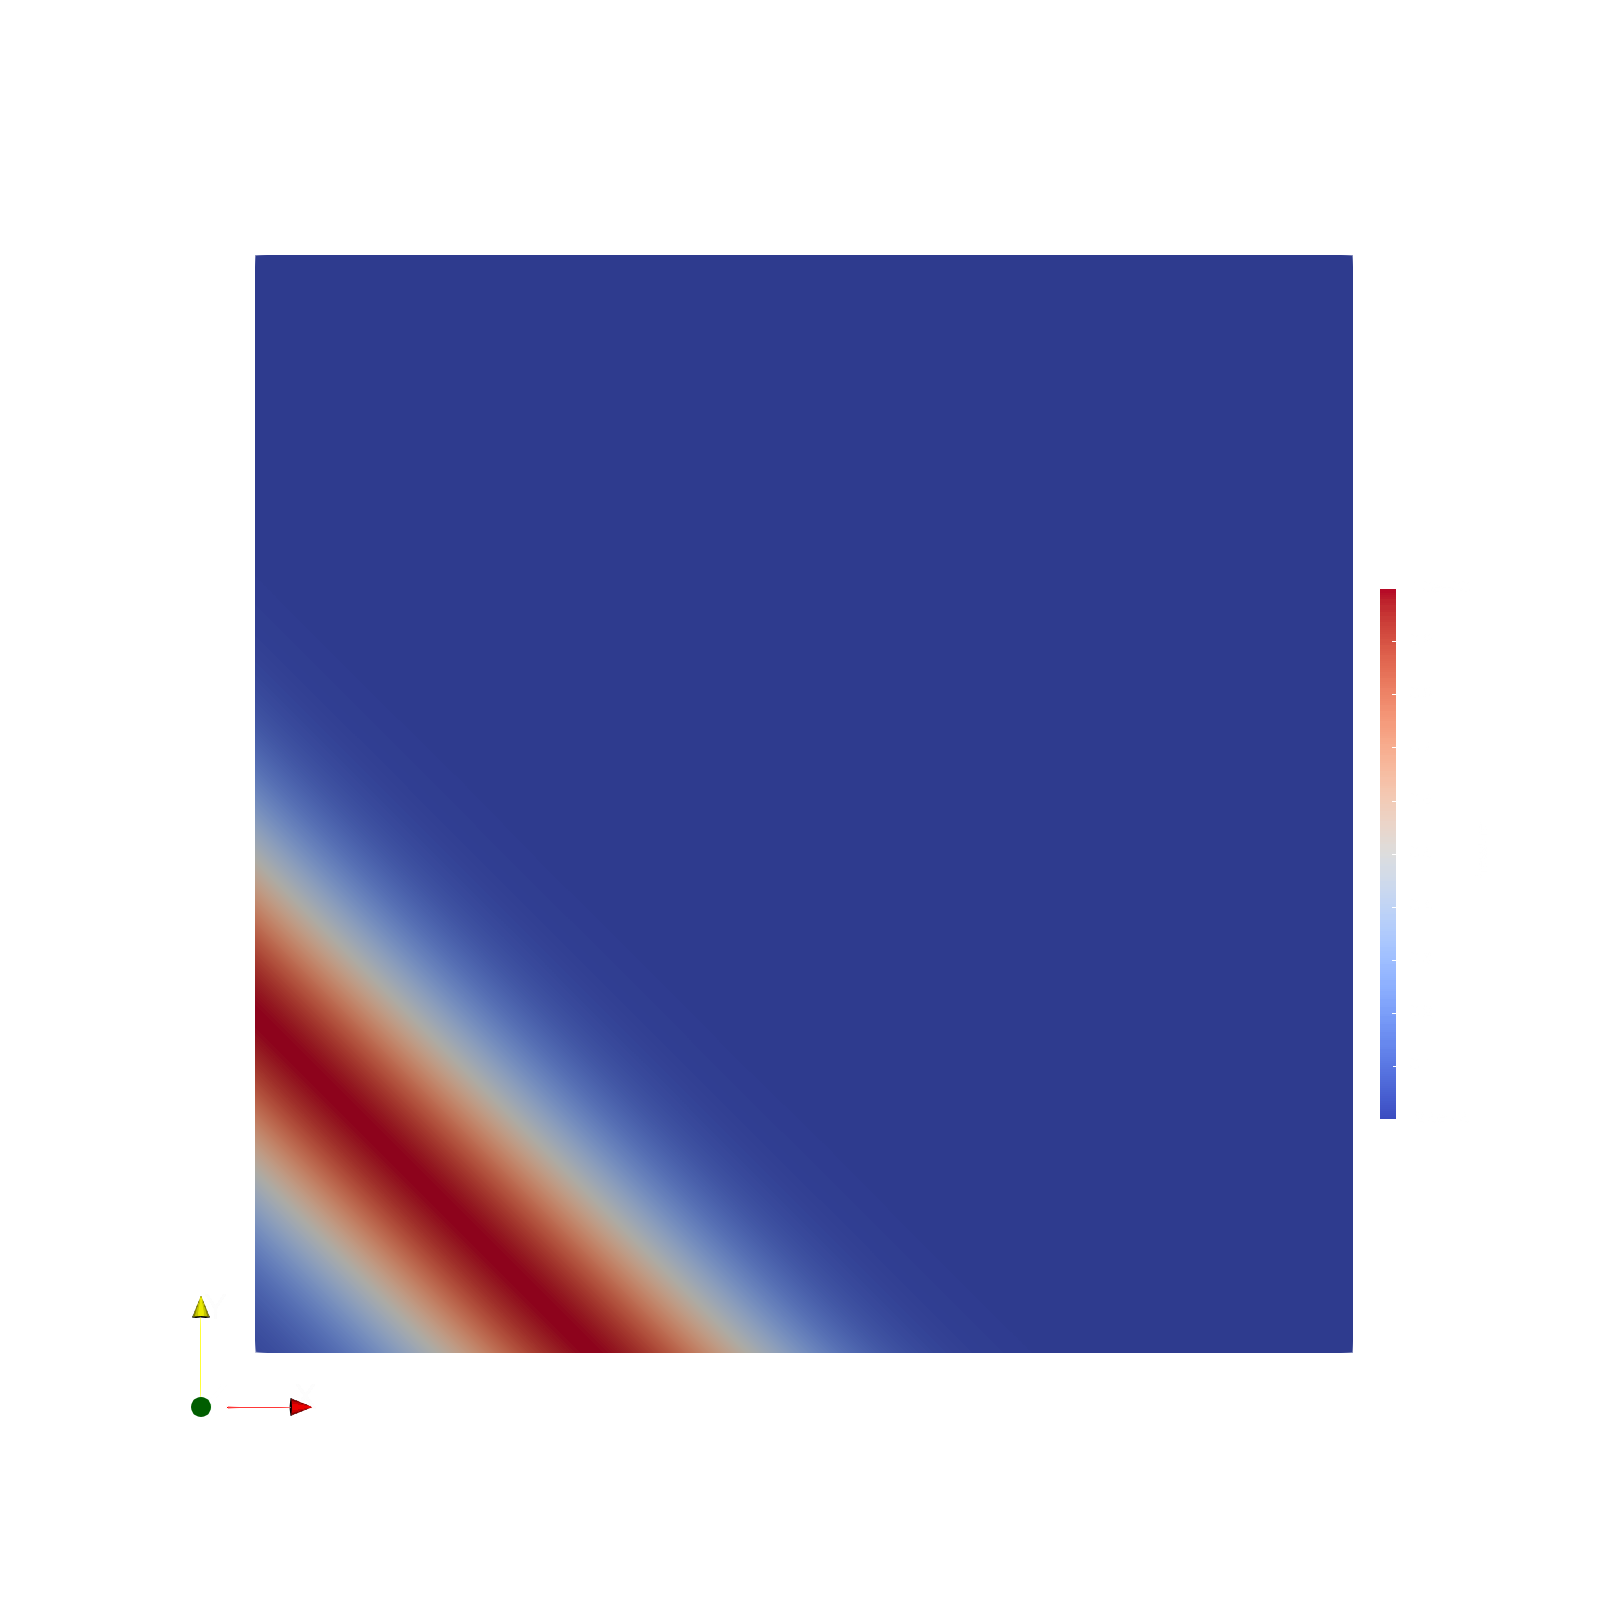
\includegraphics[width=0.6\textwidth]{Chapter_results/media/problem_1}
    \caption{Test case: A wave travels through a square domain at a 45° angle.}\label{fig:problem}
\end{figure}

\section{Scaling Tests}\label{section:results:scaling_tests}

Parallel scaling is an important aspect of the performance of a program. It describes how the
execution time varies when more resources are assigned to the problem. This is an optimisation
problem, as each problem will need a different amount of resources dedicated to it to attain the
best scaling possible. 

A completely parallelisable program, often called embarrassingly parallel, should scale linearly
with the amount of resources. The speedup \(S\) of a workload split between \(P\) workers should be
equal to the number of workers in Equation~\ref{equ:scaling}, with \(t_1\) being the time to solve
the problem serially using a single worker, and \(t_p\) being the time to solve the problem in
parallel using \(P\) workers. In this work, workers are a single \acrshort{acr:GPU} or a single
\acrshort{acr:CPU} core for comparative tests.

\begin{equation} \label{equ:scaling}
    S = \frac{t_1}{t_P}
\end{equation}

Unfortunately, it is often not possible to make a program entirely parallel. In such cases, dividing
a problem into more and more smaller tasks obeys the well-known Amdahl's law~\cite{Amdahl1967}, as
seen in Equation~\ref{equ:strong_scaling}. It splits the program into a sequential part \(s\) and a
parallel part \(l\), with only the parallel part scaling with the number of workers.

\begin{equation} \label{equ:strong_scaling}
    S = \frac{1}{s + \frac{l}{P}}
\end{equation}

This is called \textit{strong scaling}, where a fixed problem is solved using varying amount of
resources. Results of strong scaling tests of the solver are discussed in
Subsection~\ref{subsection:results:scaling_tests:strong}.

On the other hand, increased available resources can enable working on bigger problems. Gustafson
argues that modern highly parallel computers will be used to solve more complex problems instead of
solving smaller problems faster. Such a scaling is described with Equation~\ref{equ:weak_scaling}.

\begin{equation} \label{equ:weak_scaling}
    S = s + l \times P
\end{equation}

This is called \textit{weak scaling}. It describes solving a problem whose size increases with the
amount of resources, while the task size per worker stays constant. Weak scaling is tested in
Subsection~\ref{subsection:results:scaling_tests:weak}. With weak scaling a program will scale
indefinitely, with the slope of the scaling being influenced by the parallel proportion of the task.

This section will also serve as a general comparison between performance of the code on
\acrshortpl{acr:CPU} and \acrshortpl{acr:GPU}. All scaling tests have been performed on the Béluga
supercomputer. Scaling is evaluated by varying the number of \textit{nodes}, where a node in this
context is a single computer from Béluga, sporting 40 \acrshort{acr:CPU} cores and 4
\acrshortpl{acr:GPU} as stated in Subsection~\ref{subsection:results:platforms:beluga}. The
four-node execution time of those tests therefore represents the program running on 16
\acrshortpl{acr:GPU} or 160 \acrshort{acr:CPU} cores, for the \acrshort{acr:GPU} and
\acrshort{acr:CPU} computations respectively.

Both scaling tests evaluate the core solver part of the program, as the meshes start with enough
elements to have a well resolved solution all along the simulation. The \acrlong{acr:AMR} and
dynamic load balancing subroutines are still enabled. The subroutines still run their evaluation
phases, the error estimation and load imbalance computation respectively, but do not deem the
estimated error and load imbalance high enough to trigger the whole subroutine. 

\subsection{Strong scaling}\label{subsection:results:scaling_tests:strong}

The test case for this section is described in Section~\ref{section:results:test_case}. It is
divided into \(256\) elements in each of the \(x\) and \(y\) directions, for a total of \(K =
65536\) elements. The problem is then solved in parallel using a range of nodes, from one quarter
node to eight nodes. One quarter node contains \(1\) \acrshort{acr:GPU} and \(10\)
\acrshort{acr:CPU} cores, while eight nodes contain \(16\) \acrshortpl{acr:GPU} and \(160\)
\acrshort{acr:CPU} cores. The mesh is split into blocks accordingly, one block per
\acrshort{acr:GPU} or one block per \acrshort{acr:CPU} core. The first test has a polynomial order
\(N = 4\) for all elements, and a block size \(B = 32\). 

The block size, as explained in
Subsection~\ref{subsection:graphics_processing_units:architecture:programming_model}, is the number
of threads in a block of threads. Having a higher block size can speed up execution by reducing the
number of instructions to dispatch by the control flow unit of the \acrshort{acr:GPU}, because the
instructions are dispatched by block of threads. However, if the threads within a block diverge,
having a higher block size can actually lower performance. A single thread diverging will have all
the threads in its block waiting until it is finished, therefore a higher block size will have more
threads stalled when divergence occurs.

We add two ``ideal'' lines both for the \acrshort{acr:GPU} and \acrshort{acr:CPU} calculations.
These lines represent perfect scaling from a data point. The dashed and dotted line represents
perfect scaling from the first data point, one \acrshort{acr:GPU} or \(10\) \acrshort{acr:CPU}
cores. This is equivalent to halving the computation time every time the computing power doubles.
Figure~\ref{fig:strong_scaling_N4_W32} shows that the \acrshort{acr:GPU} curve is always below this
ideal line. As we increase the number of \acrshortpl{acr:GPU}, the performance scales better than
linearly up to a point, and then decreases. We therefore add a second dashed line, which represents
the scaling from the best point, where the computation time multiplied by the number of
\acrshortpl{acr:GPU} is the lowest. This line is more representative, and will be used for the next
figures.

\begin{figure}[H]
    \centering
    \includesvg[width=0.5\textwidth]{Chapter_results/media/strong_scaling_N4_K65536_W32}
    \caption{Strong scaling: The number of workers increases while the problem size stays fixed. \(N
        = 4\), \(K = 65536\), \(B = 32\)}\label{fig:strong_scaling_N4_W32}
\end{figure}

Figure~\ref{fig:strong_scaling_N4_W32} shows that the \acrshort{acr:GPU} implementation, initially
slower than the \acrshort{acr:CPU} implementation, overtakes it when one full node or more is used.
The higher number of nodes show the \acrshort{acr:GPU} implementation to be \(2.9 \times \) faster
that the \acrshort{acr:CPU} implementation.

At low numbers of \acrshortpl{acr:GPU} working on the same problem, the \acrshortpl{acr:GPU} are
more heavily loaded. It is possible that the higher memory usage, or the increased cache eviction
rate lowers the performance of \acrshortpl{acr:GPU} in that regime. With a lower number of elements
being worked on by a \acrshort{acr:GPU}, cache has to be emptied less often to make room for more
elements to use for computations.

At the end of the curve, we see that the scaling is slightly reduced. This could be a hint that the
\acrshortpl{acr:GPU} are not sufficiently loaded for those cases. These \acrshortpl{acr:GPU} have
many \acrshort{acr:CUDA} cores, \(5120\) each in the case of Béluga. If the workload does not saturate
the \acrshort{acr:GPU}, some of those cores will be idle, leading to worse performance. The best
number of elements per \acrshort{acr:GPU} seems to be around \(4096\) for this case.

The next test, shown in Figure~\ref{fig:strong_scaling_N6_W32}, shows the same test case but with an
increased polynomial order of \(N = 6\) for all elements. The rationale is that the
\acrshort{acr:GPU} should spend more time on the computations, since the computations will be
heavier, while spending the same time on the overhead of kernel calls and other housekeeping.

\begin{figure}[H]
    \centering
    \includesvg[width=0.5\textwidth]{Chapter_results/media/strong_scaling_N6_K65536_W32}
    \caption{Strong scaling: The number of workers increases while the problem size stays fixed. \(N
        = 6\), \(K = 65536\), \(B = 32\)}\label{fig:strong_scaling_N6_W32}
\end{figure}

Figure~\ref{fig:strong_scaling_N6_W32} shows that the increased polynomial order has not increased
the performance of the \acrshort{acr:GPU} implementation compared to the \acrshort{acr:CPU}
implementation, rather shifting to the right the crossover point where the \acrshort{acr:GPU}
implementation is faster. It is possible that the reduced relative performance is linked to the
increased memory used by the solution, as the needed storage scales with \({\left( 2 N + 1
\right)}^2\), where \(N\) is the polynomial order of elements.

Next, this last case is computed again with increased block size \(B\), first 64 on
Figure~\ref{fig:strong_scaling_N6_W64}, then 128 on Figure~\ref{fig:strong_scaling_N6_W128}. The
\acrshort{acr:CPU} implementation is not modified. This should assess the incidence of block size on
the solution time.

\begin{figure}[H]
    \centering
    \subfloat[\(B = 64\)]
    {\includesvg[width=0.5\textwidth]{Chapter_results/media/strong_scaling_N6_K65536_W64}\label{fig:strong_scaling_N6_W64}}
    \hfill
    \subfloat[\(B = 128\)]
    {\includesvg[width=0.5\textwidth]{Chapter_results/media/strong_scaling_N6_K65536_W128}\label{fig:strong_scaling_N6_W128}}
    \caption{Strong scaling: The number of workers increases while the problem size stays fixed. \(N
        = 6\), \(K = 65536\) (a) \(B = 64\) (b) \(B = 128\)}\label{fig:strong_scaling_N6_W64-128}
\end{figure}

As the last figure suggests, increasing the block size \(B\) does incur a performance penalty. This
is possibly caused by a high amount of thread divergence within blocks. This is consistent with how
the program is written, for example Section~\ref{section:adaptive_mesh_refinement:implementation}
shows how the projection back and forth between the elements and faces has several branching code
paths. A lot of changes in the architecture of the program would have to be made to reduce this
branching, and switch to a more data-driven approach.

One thing to note is that the curve of the \acrshort{acr:CPU} implementation on
Figures~\ref{fig:strong_scaling_N4_W32} and~\ref{fig:strong_scaling_N6_W32} is similar, whereas the
\acrshort{acr:GPU} curves from all the figures differ significantly. This is a recurring theme of
all the tests in this chapter: code running on \acrshortpl{acr:GPU} seems to be harder to optimise
and some factors have unexpected influences on the performance.

\subsection{Weak scaling}\label{subsection:results:scaling_tests:weak}

The weak scaling test uses the test case from Section~\ref{section:results:test_case}. The domain is
split up into elements such that each node contains 16384 elements. This amounts to 4096 elements
per \acrshort{acr:GPU}, or 410 elements per \acrshort{acr:CPU} core. The simulation is first
computed with the highest number of nodes, therefore the smallest elements and time step size. The
\acrshort{acr:CFL} number is adjusted for all other simulations in order to use the same time step
size, therefore the same total number of iterations. An ideal result is a flat curve, indicating
that by increasing the problem size and resources by the same amount, the simulation time stays the
same. The problem is studied from ¼ node to 16 nodes.

\begin{figure}[H]
    \centering
    \includesvg[width=0.6\textwidth]{Chapter_results/media/weak_scaling_N4_K4096_W32}
    \caption{Weak scaling: The problem size increases with the number of workers. \(N = 4\), \(K =
        16384/{node}\)}\label{fig:weak_scaling}
\end{figure}

Figure~\ref{fig:weak_scaling} shows good weak scaling from the \acrshort{acr:GPU} implementation.
Keeping in mind that the quarter node and single node cases have a reduced workload by not having to
do any \acrshort{acr:MPI} communication over the network, and the quarter node \acrshort{acr:GPU}
case has no \acrshort{acr:MPI} communication to do at all, the \acrshort{acr:GPU} curve is
reasonably flat. The \acrshort{acr:CPU} curve is not as good, indicating that there may be a
bottleneck in the communication part of the program. The \acrshort{acr:CPU} implementation has a
much higher number of workers than the \acrshort{acr:GPU} one, \(40\) per node instead of four,
increasing the inter-process communication needed. The slope of the \acrshort{acr:CPU} curve is
about \(0.4\) with respect to the number of \acrshort{acr:CPU} cores. 

\section{Adaptive Mesh Refinement Performance}\label{section:results:adaptivity_performance}

This section establishes the performance of the \acrlong{acr:AMR}. The problem from
Section~\ref{section:results:test_case} is used, initially split into four elements in each of the
\(x\) and \(y\) directions, for a total of \(K = 16\) elements. The initial polynomial order is \(N
= 4\). The system is allowed to refine up to a split level \(S = 5\), meaning a cell can split five
times and become \(\frac{1}{32}\) of the size of the original cell, and up to a polynomial order \(N
= 16\). The target error threshold is set to \num{1e-6}, meaning it will refine elements whose
estimated error is greater than that number.

\Acrlong{acr:AMR} is a costly process, as the \acrshort{acr:CPU} must reallocate arrays on the
\acrshort{acr:GPU} for the different objects making up the mesh, and then schedule kernels to move
objects to the new arrays. We test here two strategies to reduce the performance overhead of
\acrlong{acr:AMR}, while reducing error. 

First, \acrlong{acr:AMR} will be performed at a regular interval.
Figures~\ref{fig:adaptivity_efficiency_A5},~\ref{fig:adaptivity_efficiency_A20},~\ref{fig:adaptivity_efficiency_A100}
and~\ref{fig:adaptivity_efficiency_A500} show the results of refining the mesh every \(5\), \(20\),
\(100\) and \(500\) timesteps, respectively.

Secondly, the simulations are performed with an increasing number of refinement pre-condition steps
as described in Section~\ref{section:adaptive_mesh_refinement:pre_conditioning}. The analysis ranges
from no pre-condition step to five steps. The total simulation time is shown in blue. It is the sum
of the time taken up by the pre-condition of the mesh, shown in green, and the computation time to
solve the problem, shown in yellow. 

We compare those simulations to two non-adaptive cases. In the first case, the initial mesh is fully
refined uniformly up to the maximum level attained by the adaptive cases. The mesh is split into
\(128\) elements in each of the \(x\) and \(y\) dimensions, for a total of \(K = 16384\) elements,
with a polynomial order \(N = 10\). This result is shown as a dashed line on the figures. The second
non-adaptive case aims to obtain a maximum error similar to the adaptive case. The mesh is refined
uniformly to \(32\) elements in each of the \(x\) and \(y\) dimensions, for a total of \(K = 1024\)
elements, with a polynomial order \(N = 10\). This case is shown as a dotted line on the figures.
Both the simulation time and the error relative to the analytical solution are plotted. The cases
were computed using the Narval supercomputer on a single \acrshort{acr:GPU}.

\begin{figure}[H]
    \centering
    \subfloat[Solution time]
    {\includesvg[width=0.49\textwidth]{Chapter_results/media/adaptivity_time_N4_K16_A5}\label{fig:adaptivity_efficiency_A5_time}}
    \subfloat[Maximum error]
    {\includesvg[width=0.49\textwidth]{Chapter_results/media/adaptivity_error_N4_K16_A5}\label{fig:adaptivity_efficiency_A5_error}}
    \caption{\Acrlong{acr:AMR} performance: Simulation time and error for increasing number of pre-condition steps. \(N_{initial} = 4\), \(K_{initial} = 16\), \(S = 5\), refinement interval = 5}\label{fig:adaptivity_efficiency_A5}
\end{figure}

\begin{figure}[H]
    \centering
    \subfloat[Solution time]
    {\includesvg[width=0.49\textwidth]{Chapter_results/media/adaptivity_time_N4_K16_A20}\label{fig:adaptivity_efficiency_A20_time}}
    \hfill
    \subfloat[Maximum error]
    {\includesvg[width=0.49\textwidth]{Chapter_results/media/adaptivity_error_N4_K16_A20}\label{fig:adaptivity_efficiency_A20_error}}
    \caption{\Acrlong{acr:AMR} performance: Simulation time and error for increasing number of pre-condition steps. \(N_{initial} = 4\), \(K_{initial} = 16\), \(S = 5\), refinement interval = 20}\label{fig:adaptivity_efficiency_A20}
\end{figure}

\begin{figure}[H]
    \centering
    \subfloat[Solution time]
    {\includesvg[width=0.49\textwidth]{Chapter_results/media/adaptivity_time_N4_K16_A100}\label{fig:adaptivity_efficiency_A100_time}}
    \hfill
    \subfloat[Maximum error]
    {\includesvg[width=0.49\textwidth]{Chapter_results/media/adaptivity_error_N4_K16_A100}\label{fig:adaptivity_efficiency_A100_error}}
    \caption{\Acrlong{acr:AMR} performance: Simulation time and error for increasing number of pre-condition steps. \(N_{initial} = 4\), \(K_{initial} = 16\), \(S = 5\), refinement interval = 100}\label{fig:adaptivity_efficiency_A100}
\end{figure}

\begin{figure}[H]
    \centering
    \subfloat[Solution time]
    {\includesvg[width=0.49\textwidth]{Chapter_results/media/adaptivity_time_N4_K16_A500}\label{fig:adaptivity_efficiency_A500_time}}
    \hfill
    \subfloat[Maximum error]
    {\includesvg[width=0.49\textwidth]{Chapter_results/media/adaptivity_error_N4_K16_A500}\label{fig:adaptivity_efficiency_A500_error}}
    \caption{\Acrlong{acr:AMR} performance: Simulation time and error for increasing number of pre-condition steps. \(N_{initial} = 4\), \(K_{initial} = 16\), \(S = 5\), refinement interval = 500}\label{fig:adaptivity_efficiency_A500}
\end{figure}

From
Figures~\ref{fig:adaptivity_efficiency_A5},~\ref{fig:adaptivity_efficiency_A20},~\ref{fig:adaptivity_efficiency_A100}
and~\ref{fig:adaptivity_efficiency_A500}, we see that this is an optimisation problem, with
tradeoffs between the simulation time and the error generated.

An important part of the error comes from the initial conditions being applied on too coarse a mesh.
Even if the mesh is refined, this error propagates through the domain. Mesh pre-condition, as
described in Section~\ref{section:adaptive_mesh_refinement:pre_conditioning}, aims to alleviate this
problem. Indeed, with enough pre-condition steps all cases converge to an acceptable error. Adding
more pre-condition steps does not improve the results, as the target error threshold of \num{1e-6}
is likely reached.

The fully refined non-adaptive case, shown in dashed lines on
Figures~\ref{fig:adaptivity_efficiency_A5},~\ref{fig:adaptivity_efficiency_A20},~\ref{fig:adaptivity_efficiency_A100}
and~\ref{fig:adaptivity_efficiency_A500}, is prohibitively time consuming to compute. The solution
is well resolved as shown on Figure~\ref{fig:adaptivity_efficiency_A20_error}, with the analytical
solution error being \(19 \times \) smaller than in the adaptive case. On the other hand, it takes
\(22 \times \) as much time to compute. The difference is even more pronounced when the refinement
interval is increased to \(100\), as in Figure~\ref{fig:adaptivity_efficiency_A100_time}, where the
adaptive solution with three to five pre-condition steps is around \(67 \times \) faster, at the
expense of a worse error compared to the \(20\) refinement interval case.

As for the similar maximum error non-adaptive case, shown with dotted lines, the results are closer.
The case with a refinement interval of 20 on Figure~\ref{fig:adaptivity_efficiency_A20} was used to
set the target error for that non-adaptive case. The adaptive case starting from a coarse mesh is
able to reach a similar maximum error and similar computation time when compared to the non-adaptive
case. The other cases also attain the target error threshold of \num{1e-6} while being faster.

The non-adaptive cases are closer to being ideal for the \acrshort{acr:GPU} architecture. The
non-adaptive cases have less thread divergence than the adaptive case. There is a lot more branching
in the adaptive case, with elements having a different polynomial order, non-conforming interfaces,
and different numbers of neighbours. This increased divergence lowers the performance since some
threads are predicated off while others execute an instruction. The memory access patterns of the
non-adaptive cases are also better, for example the different faces connecting to an element are
closer in memory. Threads from a same warp accessing memory that is not contiguous must perform
several memory fetches. The non-adaptive cases play to the strengths of the \acrshortpl{acr:GPU},
yet the adaptive case shows performance improvements. This means that \acrshort{acr:AMR} is worth it
even if the \acrshort{acr:GPU} architecture is not perfectly suited for it, and with improvements to
fit it better it could perform even better. Section~\ref{section:conclusion:future_work} discusses
some improvements to make the program even better suited for the \acrshort{acr:GPU} architecture.

The best number of pre-condition steps seems to be four for this case, as the target error is
reached with all refinement intervals. After this number of steps the solution does not change much
as the target error threshold is likely reached. We use that number of steps to compare the effects
of different refinement intervals in Figure~\ref{fig:adaptivity_efficiency_C4}.

\begin{figure}[H]
    \centering
    \subfloat[Solution time]
    {\includesvg[width=0.49\textwidth]{Chapter_results/media/adaptivity_time_N4_K16_C4}\label{fig:adaptivity_efficiency_C4_time}}
    \hfill
    \subfloat[Maximum error]
    {\includesvg[width=0.49\textwidth]{Chapter_results/media/adaptivity_error_N4_K16_C4}\label{fig:adaptivity_efficiency_C4_error}}
    \caption{\Acrlong{acr:AMR} performance: Simulation time and error for four pre-condition steps and increasing refinement interval. \(N_{initial} = 4\), \(K_{initial} = 16\), \(S = 5\), pre-condition steps = 4}\label{fig:adaptivity_efficiency_C4}
\end{figure}

Figure~\ref{fig:adaptivity_efficiency_C4} gives a good overview of the \acrshort{acr:AMR}
performance. All refinement intervals attain the target error threshold of \num{1e-6}, and obtain a
real maximum error under \num{1e-6} when compared to the analytical solution. 

It is always faster to use \acrshort{acr:AMR} than to start with a uniform fully refined mesh, and
it is faster to use \acrshort{acr:AMR} than a uniformly refined mesh that has the same maximum
solution error. The adaptive case can refine elements where they are most needed, saving computing
resources.

There is a balance to be made between refining often and spending more time in the
\acrshort{acr:AMR} routine, and refining less often therefore using a less refined mesh for longer.
Section~\ref{section:conclusion:future_work} discusses ideas for alternative approaches to choose
when to refine. In this case it seems that performing \acrshort{acr:AMR} every \(20\) time steps
yields the lowest error, while waiting \(100\) timesteps between refinements yields a faster runtime
at the price of a worse error that still stays below the target error threshold we set.

\section{Dynamic Load Balancing Performance}\label{section:results:load_balancing_performance}

This section is dedicated to benchmarking the dynamic load balancing module of the program in
adaptive cases where varying levels of load imbalance are generated. The sample problem is the same
as described in Section~\ref{section:results:test_case}, except that the domain size is increased
from a size of 1 to 100 in either dimension. The wave stays the same, effectively only staying in
the lower left corner during the program runtime. The program advances the solution to a simulation
time of two seconds. The mesh is split into 128 elements in each of the \(x\) and \(y\) directions,
for a total of \(K = 16384\) elements. The initial polynomial order is \(N = 4\). The problem is
solved using four \acrshort{acr:GPU} nodes from the Narval supercomputer, for a total of \(P = 16\)
\acrshortpl{acr:GPU}. This initially amounts to 1024 elements per \acrshort{acr:GPU}. The mesh is
refined every 20 timesteps. In order to prescribe a different load imbalance for different cases, a
different maximum split level \(S\) is set. This parameter controls how many times an element can
h-refine. Three cases are presented, a low load imbalance case with \(S = 3\) shown in
Figures~\ref{fig:load_imbalance_case_low_p} and~\ref{fig:load_imbalance_case_low_s}, a medium load
imbalance case with \(S = 5\) shown in Figures~\ref{fig:load_imbalance_case_medium_p}
and~\ref{fig:load_imbalance_case_medium_s}, and a high load imbalance case with \(S = 7\) shown in
Figures~\ref{fig:load_imbalance_case_high_p} and~\ref{fig:load_imbalance_case_high_s}. The different
cases are allowed to refine up to their respective maximum split level \(S\), and up to a polynomial
order of \(N = 12\). 

\begin{figure}[H]
    \centering
    \subfloat[Full domain]
    {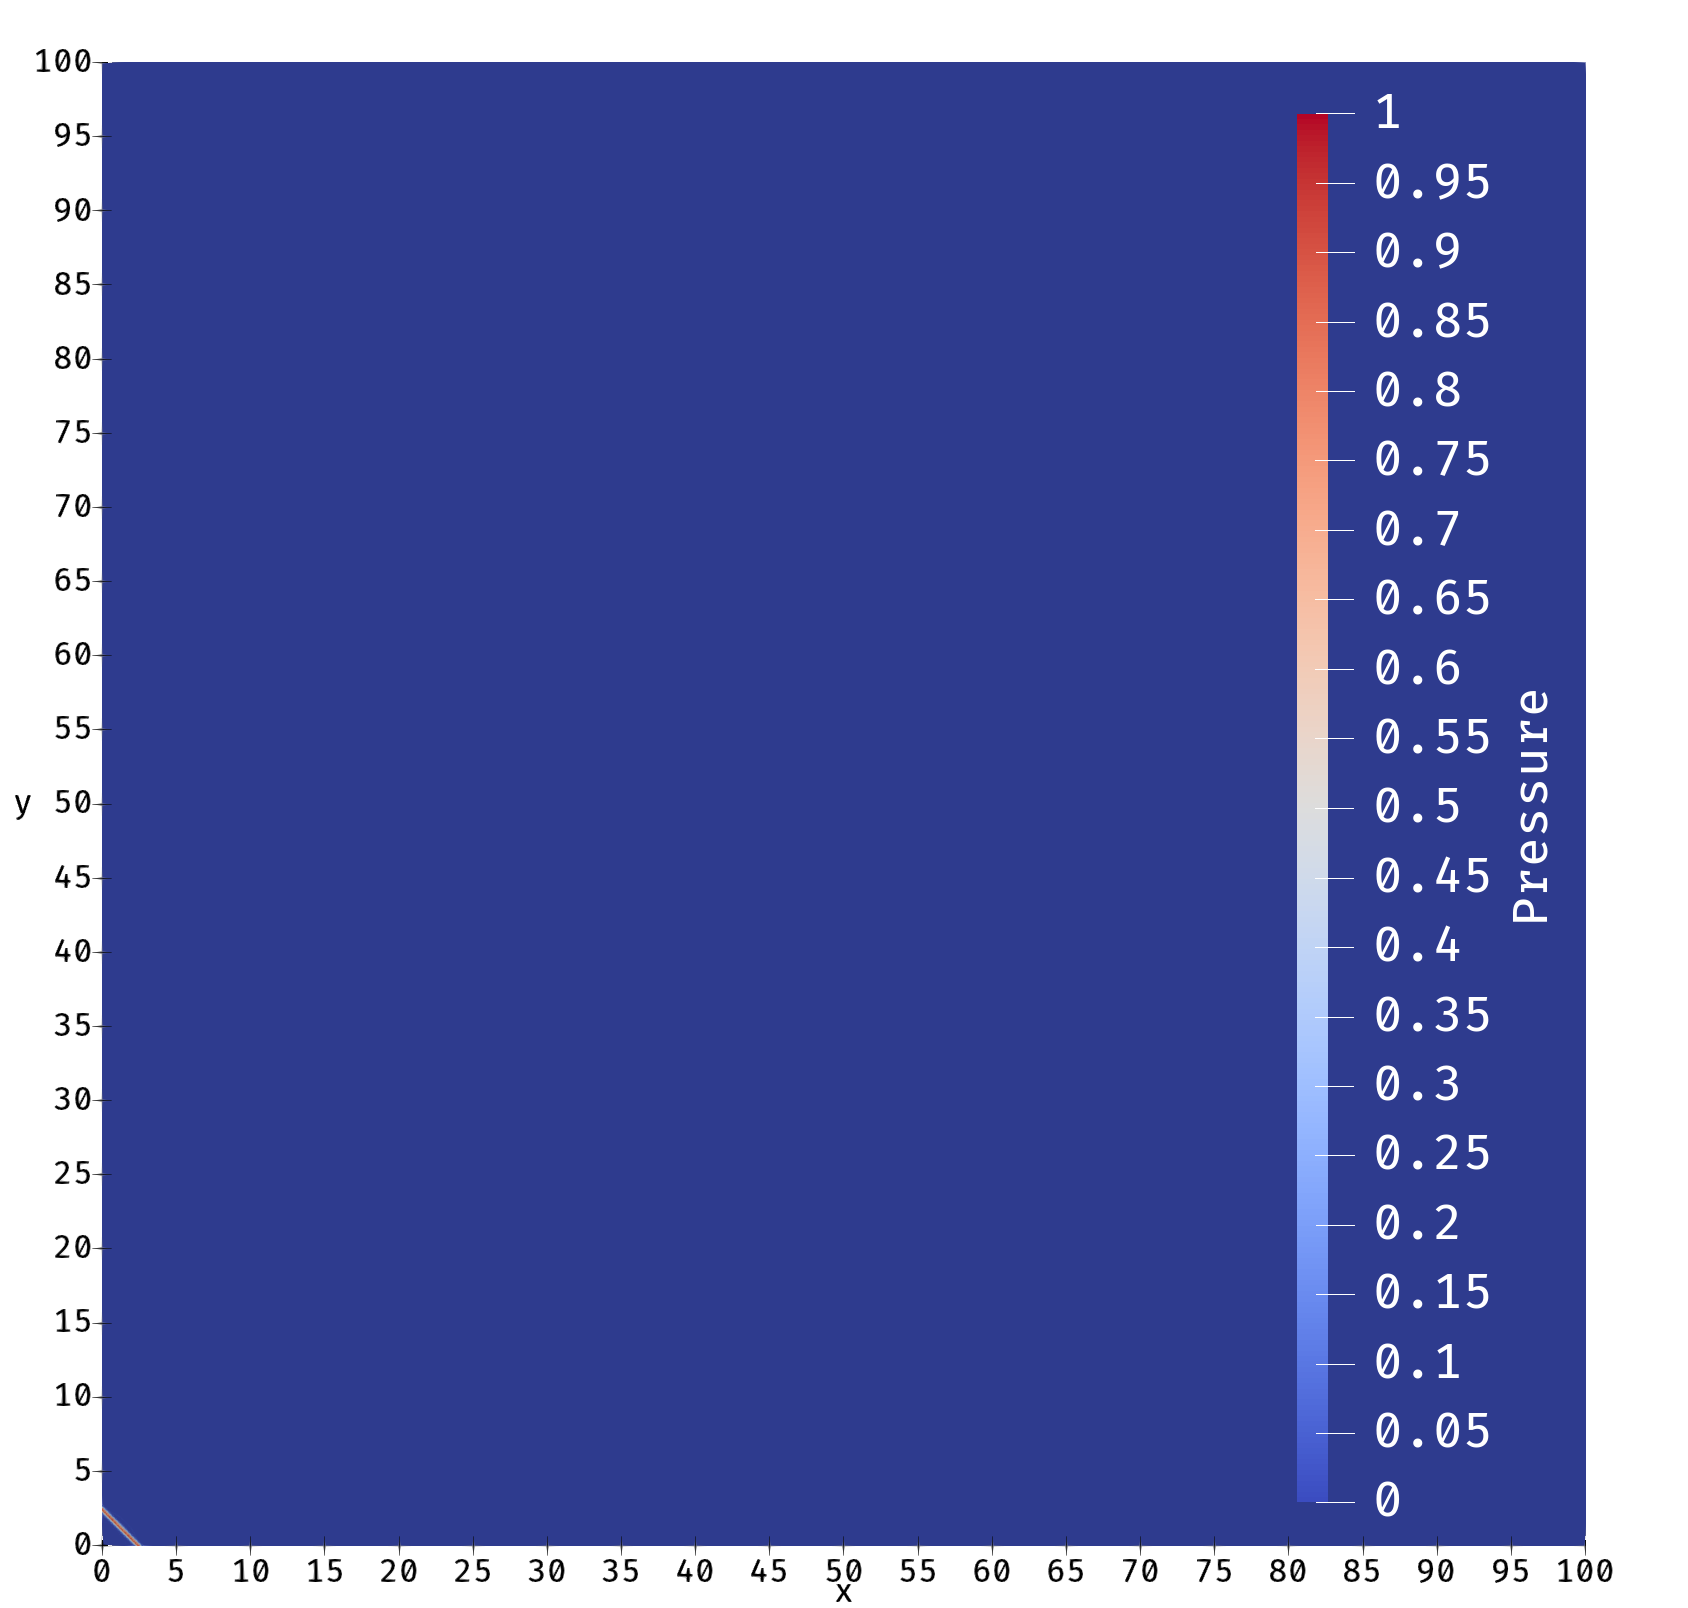
\includegraphics[width=0.5\textwidth]{Chapter_results/media/problem_low_far}\label{fig:load_imbalance_case_low_p_far}}
    \hfill
    \subfloat[Detail]
    {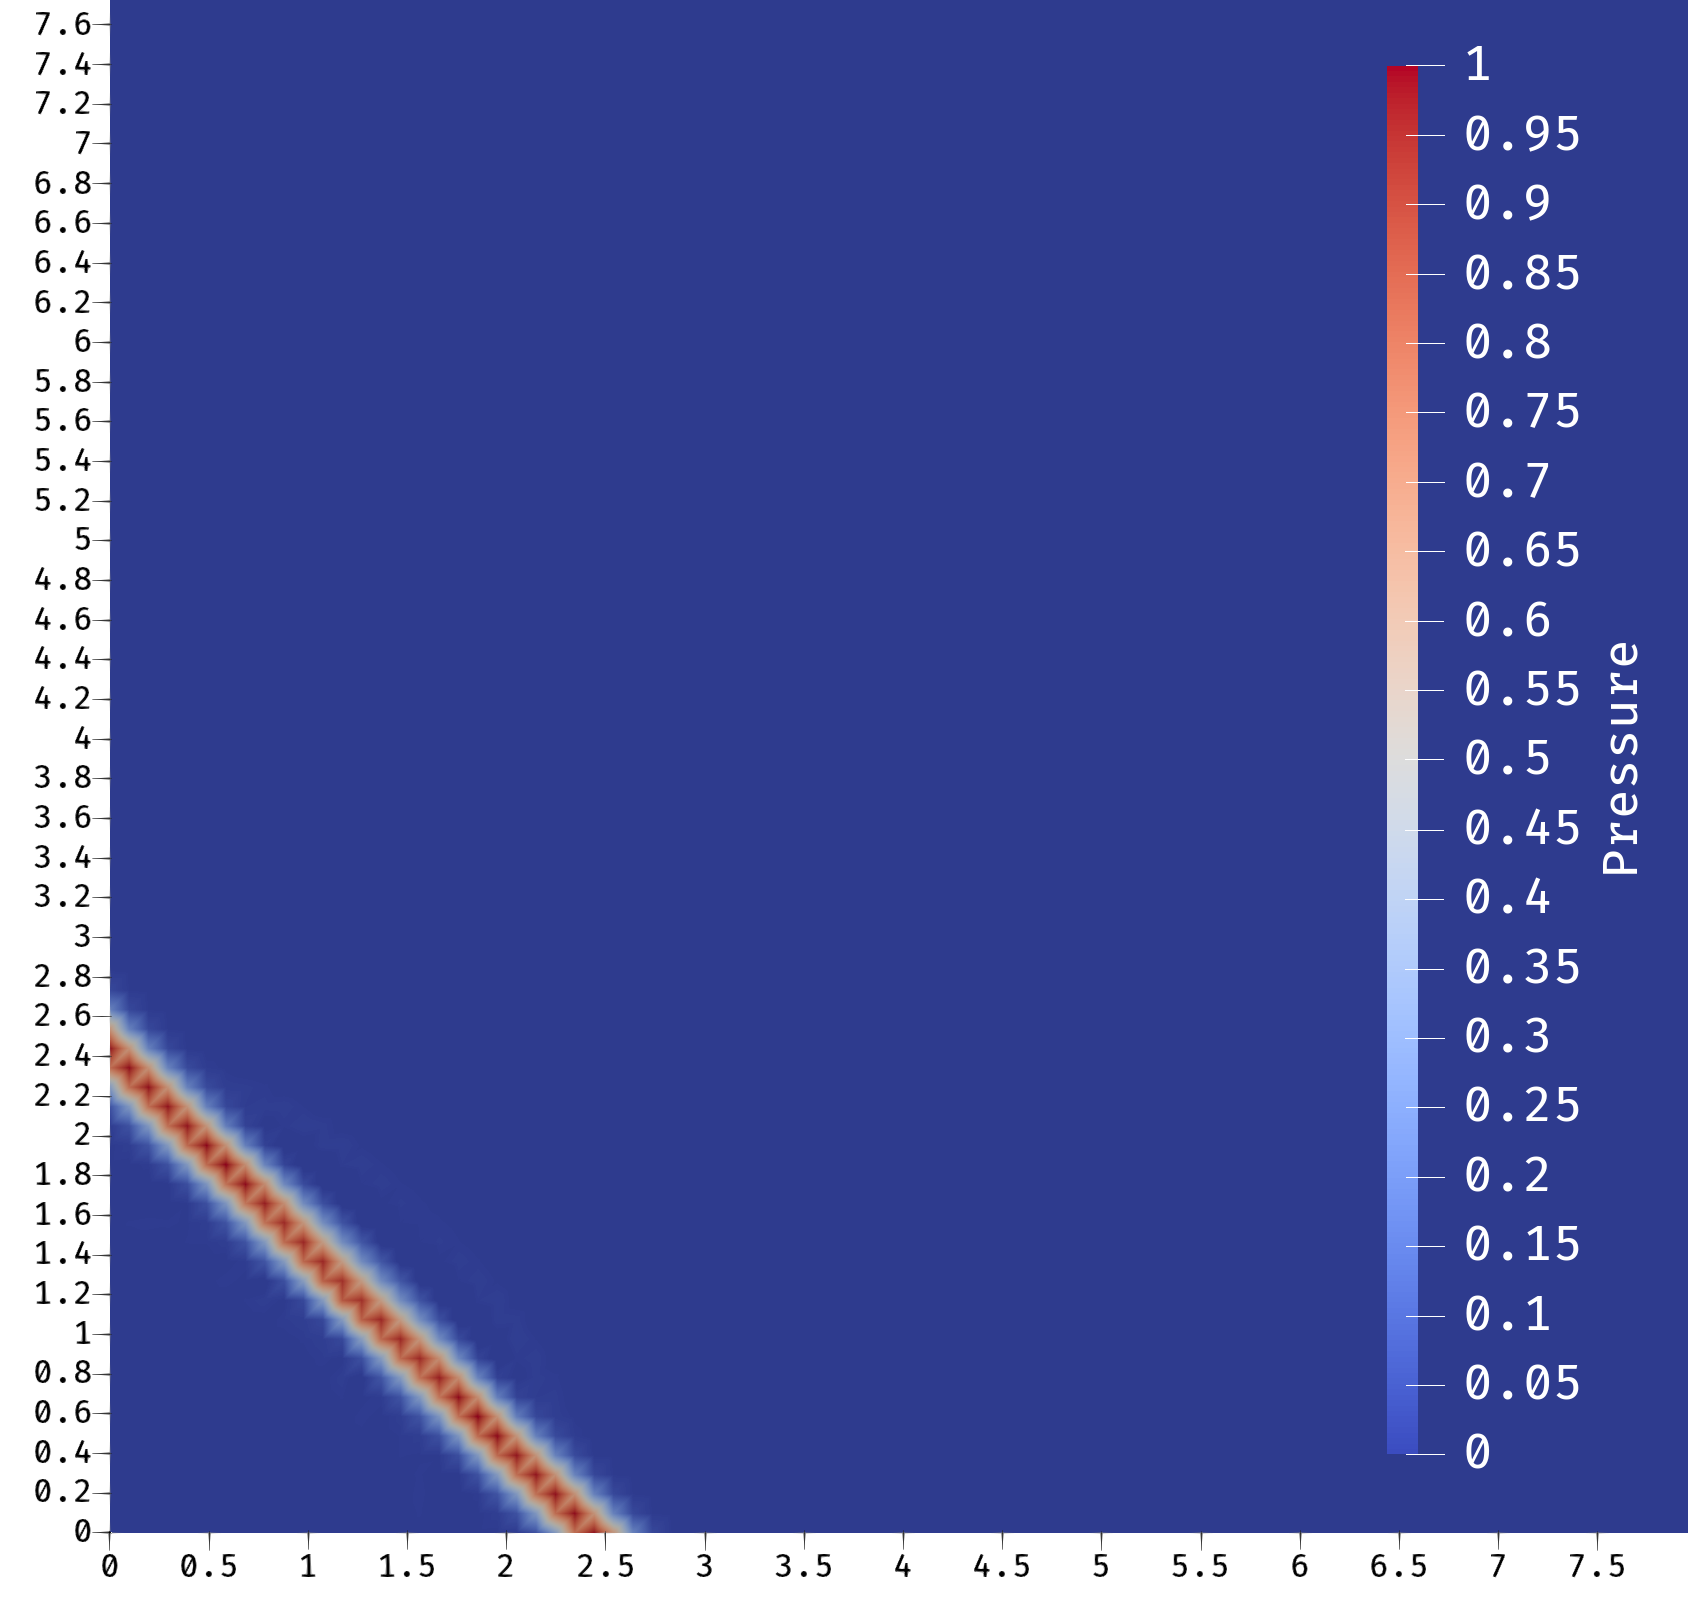
\includegraphics[width=0.48\textwidth]{Chapter_results/media/problem_low_near}\label{fig:load_imbalance_case_low_p_near}}
    \caption{Low load imbalance (\(S = 3\)) test case pressure: A wave passes through a very big domain. \(K_{initial} = 16384\), \(K_{final} = 17752\) (a) Complete domain (b) Area of interest}\label{fig:load_imbalance_case_low_p}
\end{figure}

\begin{figure}[H]
    \centering
    \subfloat[Full domain]
    {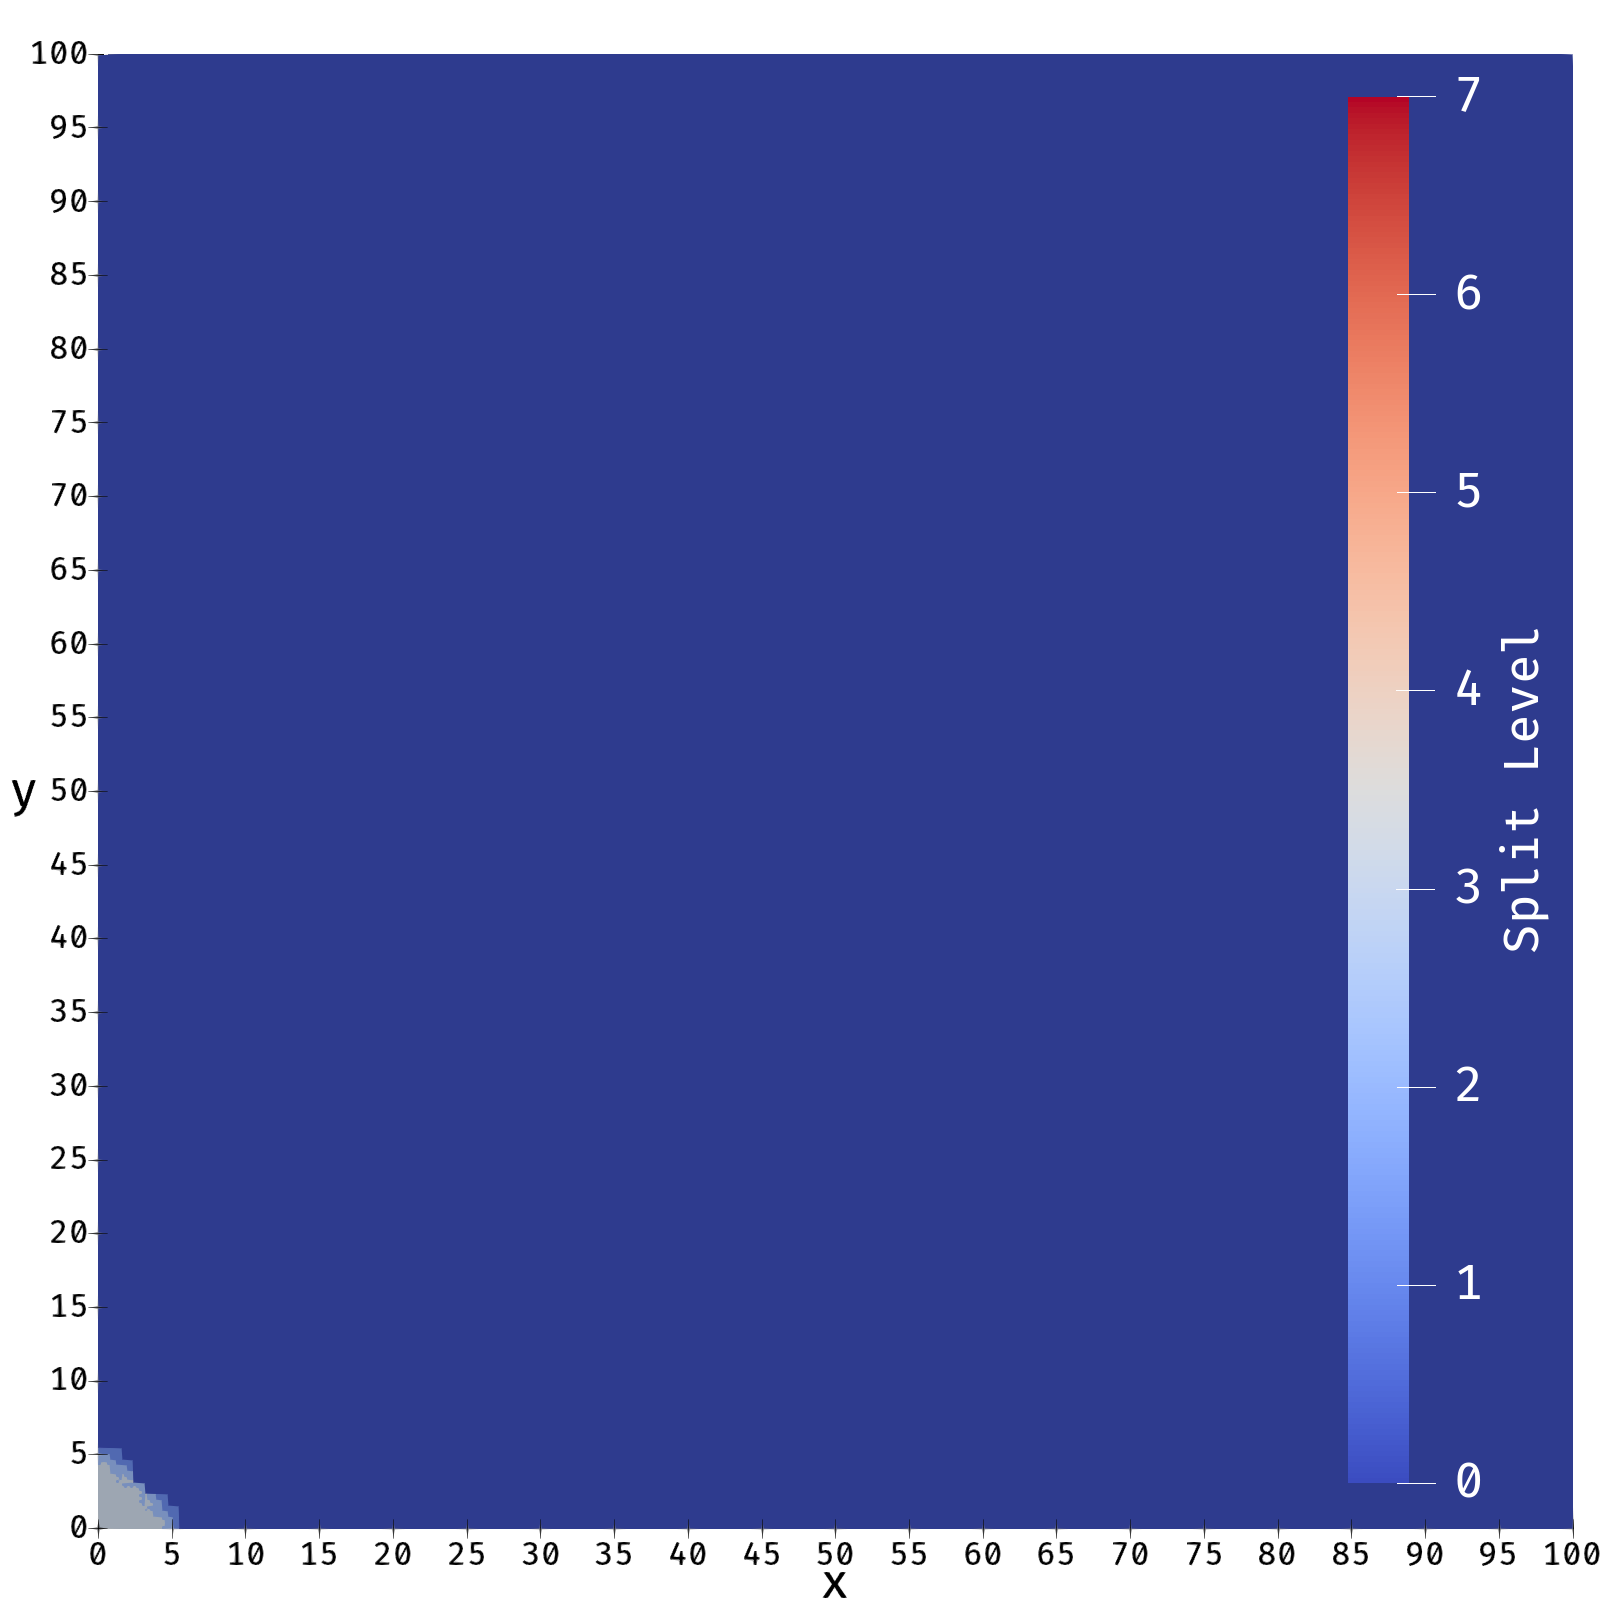
\includegraphics[width=0.5\textwidth]{Chapter_results/media/split_level_low_far}\label{fig:load_imbalance_case_low_s_far}}
    \hfill
    \subfloat[Detail]
    {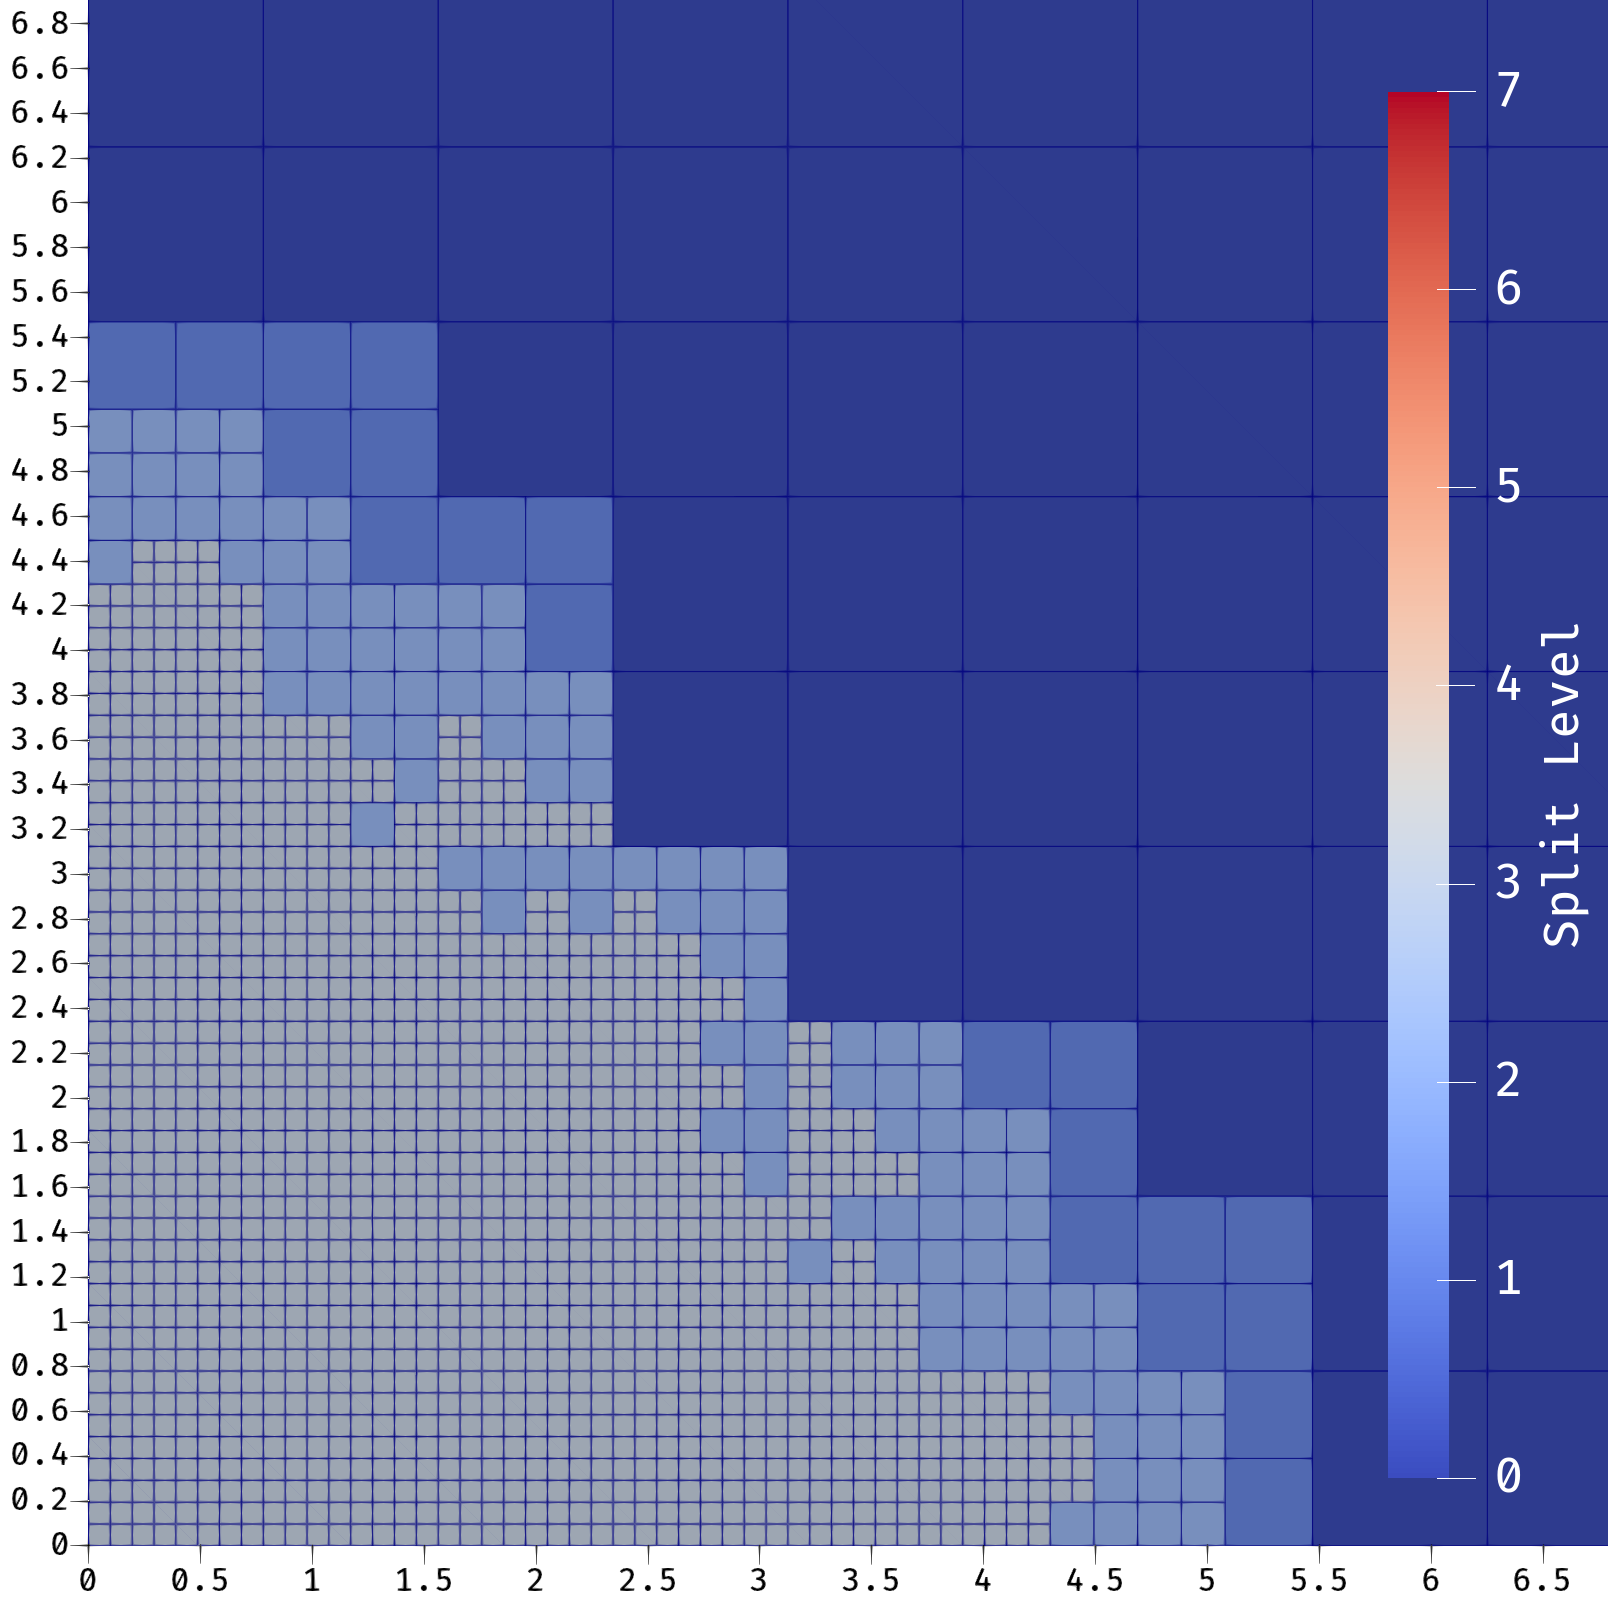
\includegraphics[width=0.48\textwidth]{Chapter_results/media/split_level_low_near}\label{fig:load_imbalance_case_low_s_near}}
    \caption{Low load imbalance (\(S = 3\)) test case split level: Split level, indicating how many times the elements have split, only the bottom left refines. \(K_{initial} = 16384\), \(K_{final} = 17752\) (a) Complete domain (b) Area of interest}\label{fig:load_imbalance_case_low_s}
\end{figure}

\begin{figure}[H]
    \centering
    \subfloat[Full domain]
    {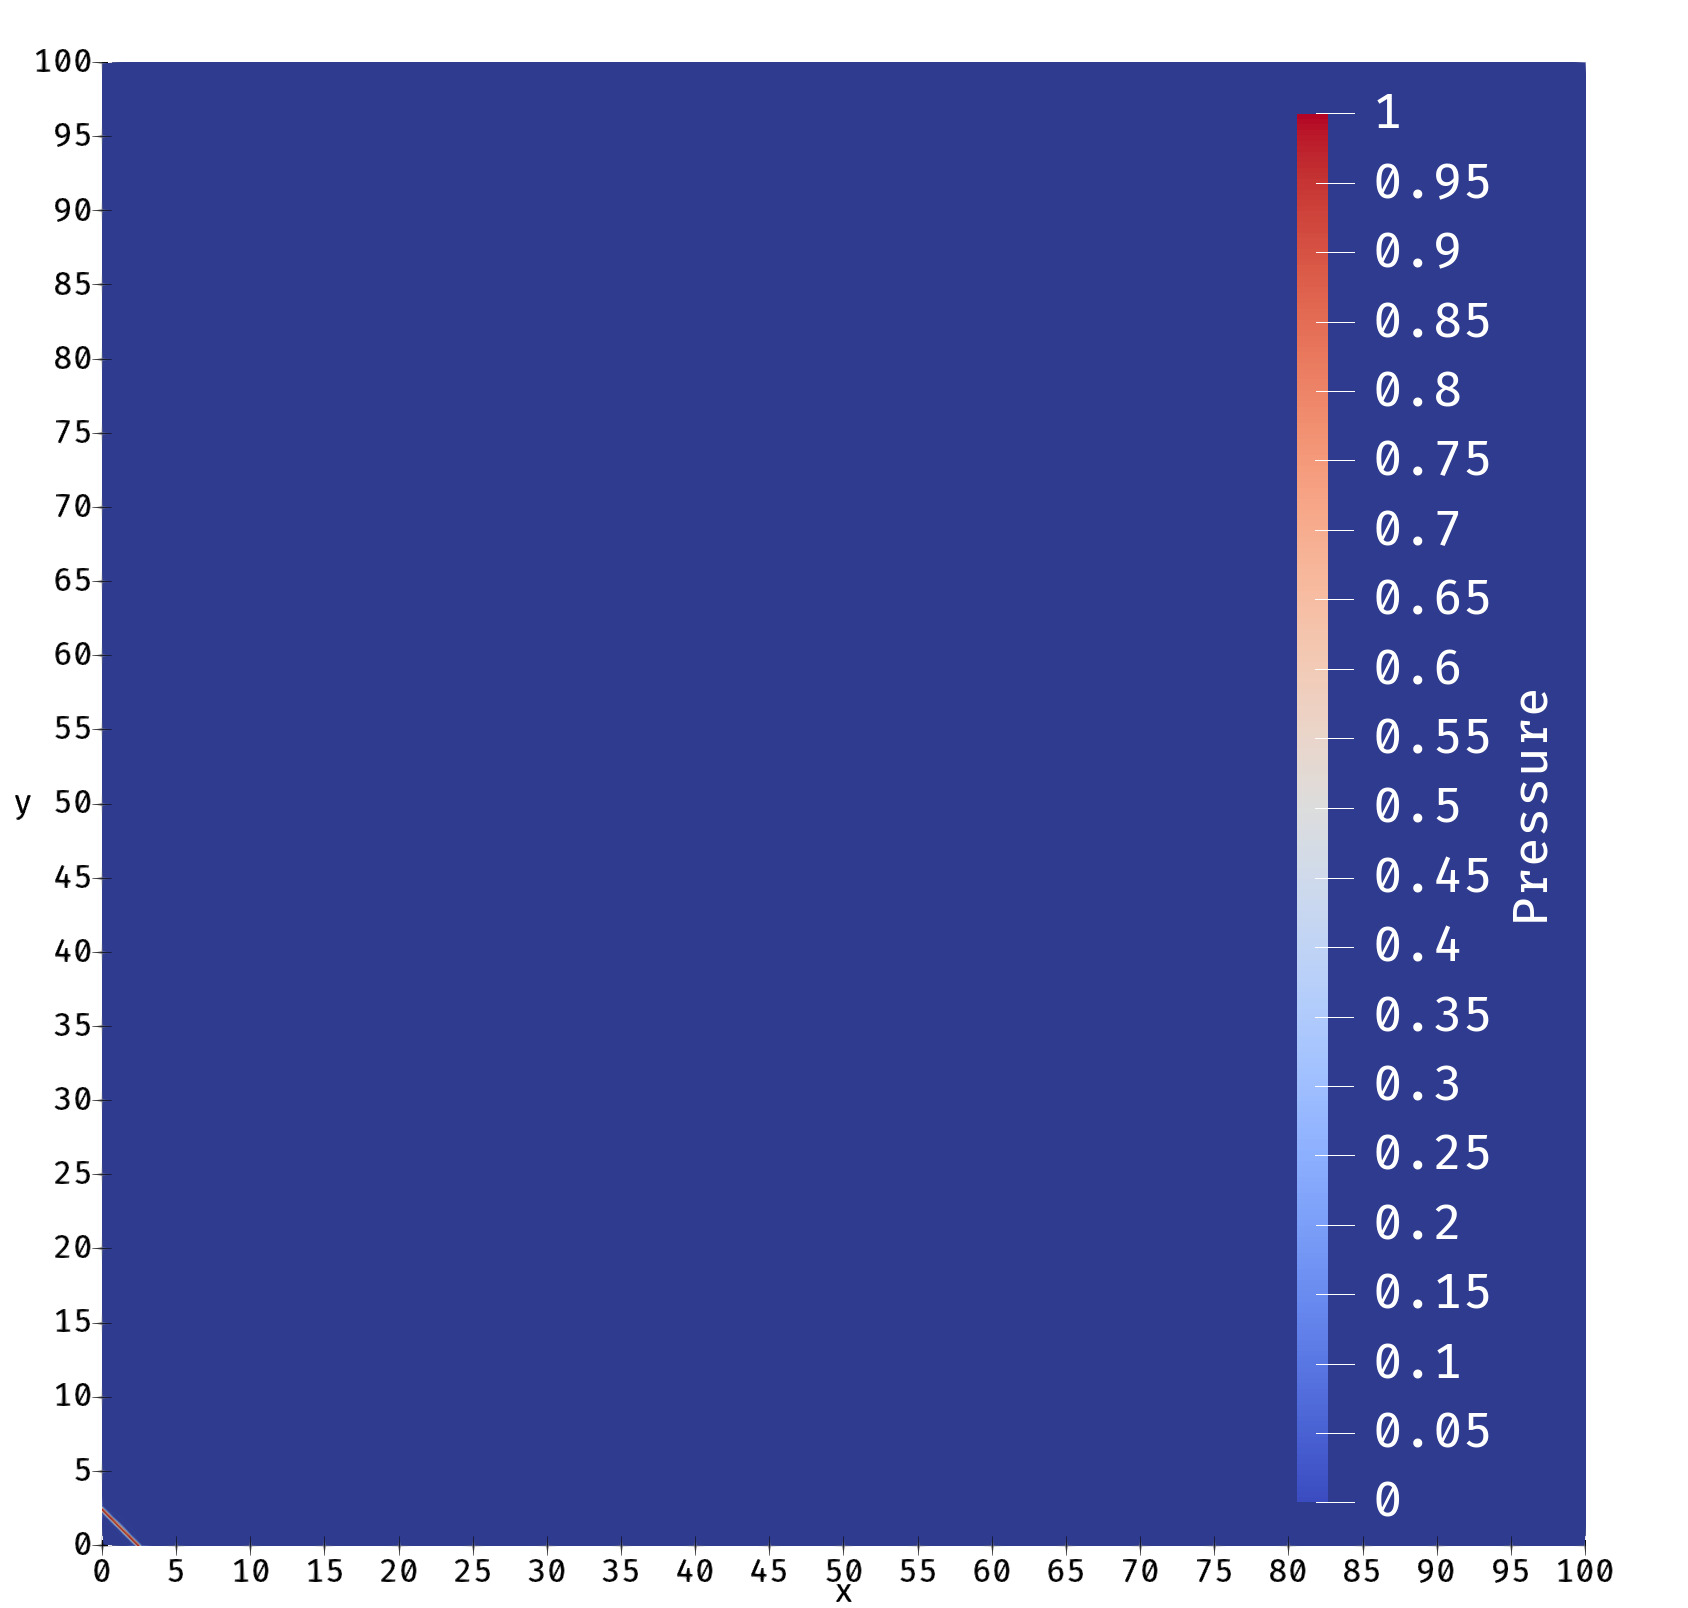
\includegraphics[width=0.5\textwidth]{Chapter_results/media/problem_medium_far}\label{fig:load_imbalance_case_medium_p_far}}
    \hfill
    \subfloat[Detail]
    {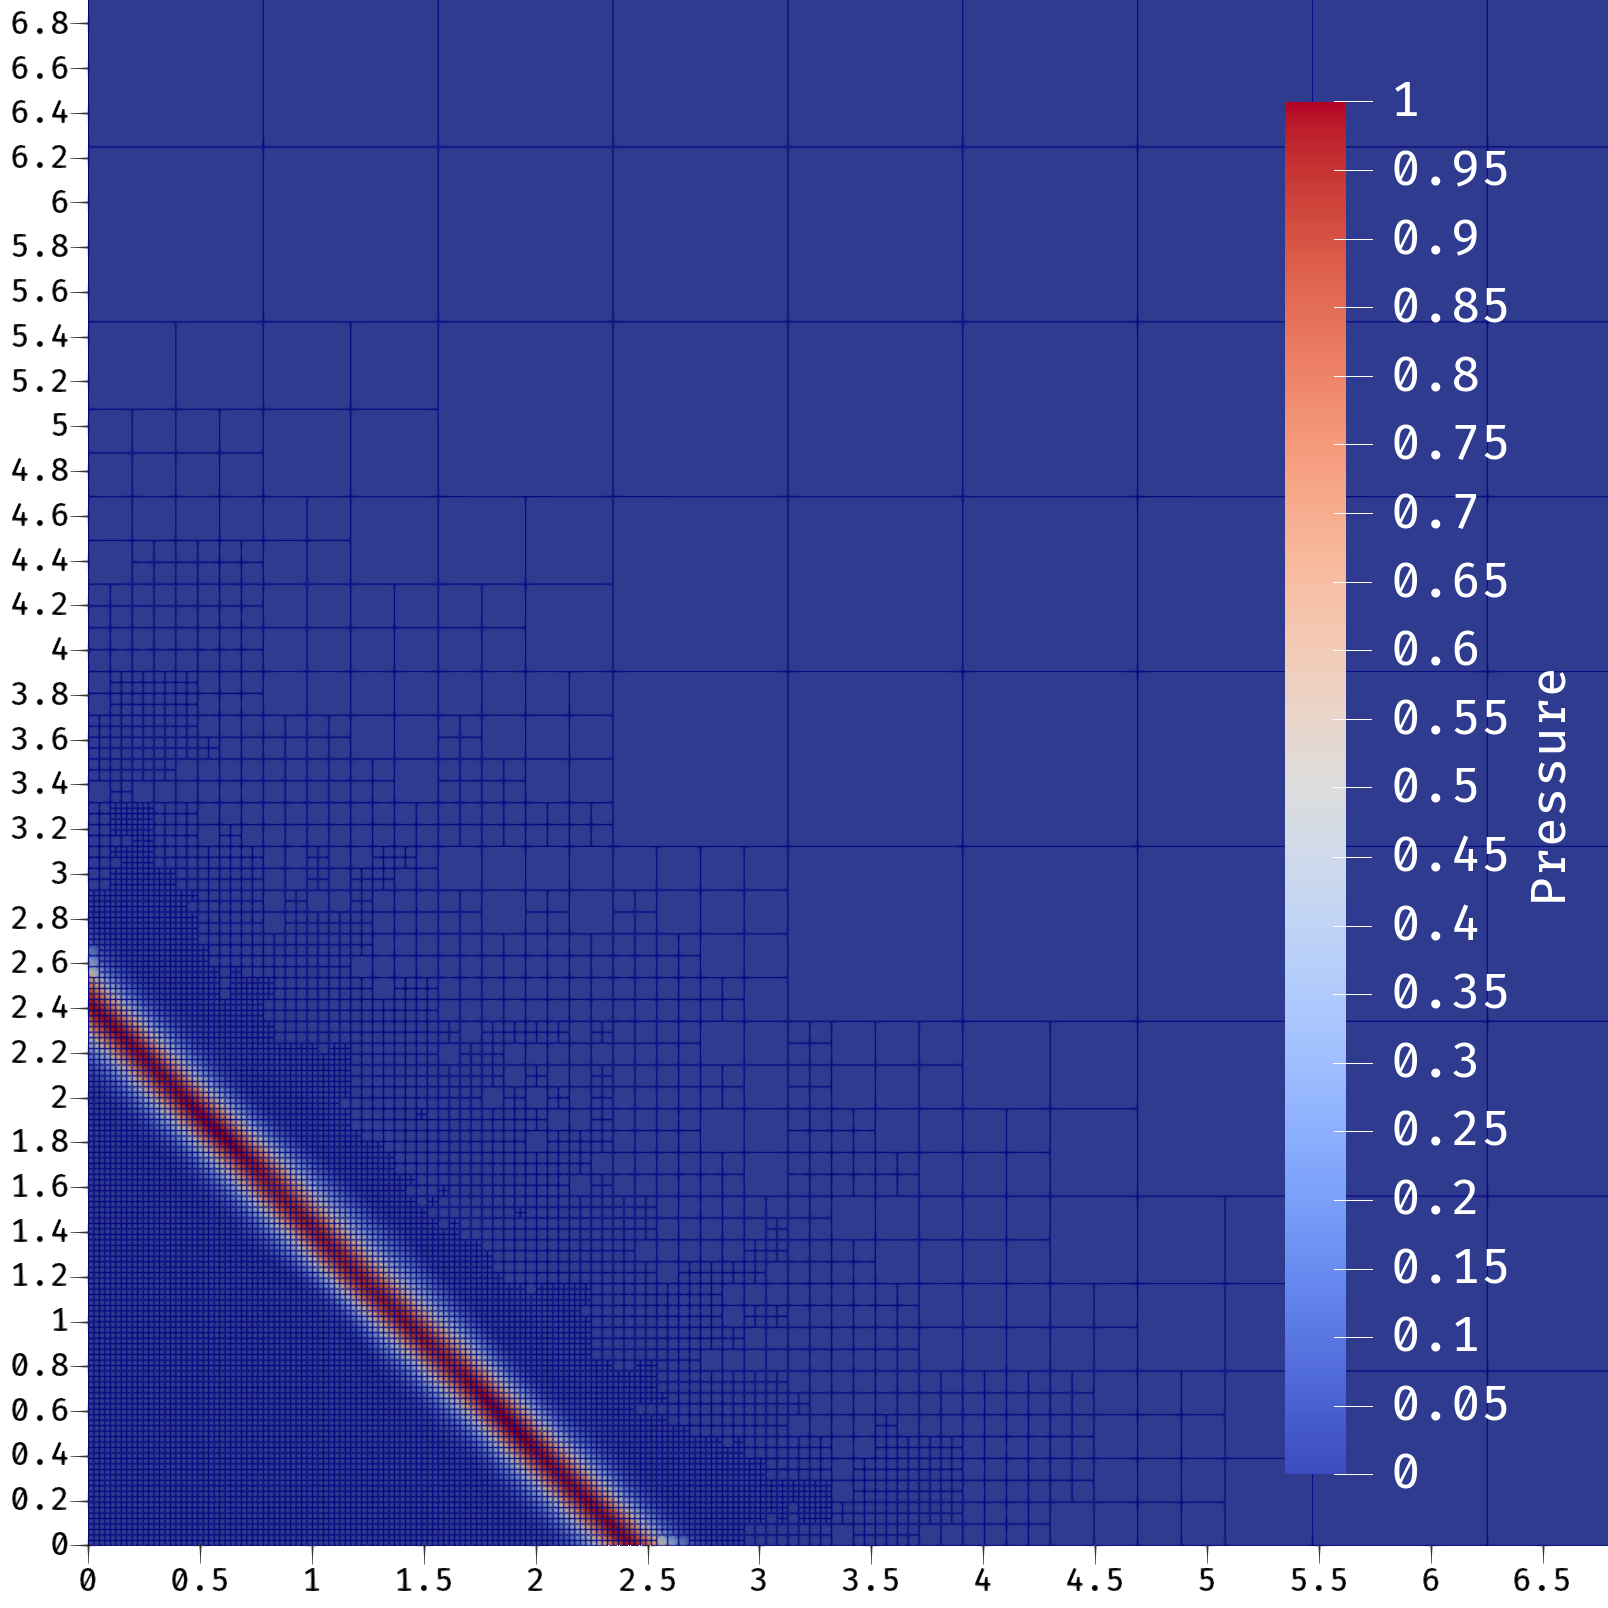
\includegraphics[width=0.48\textwidth]{Chapter_results/media/problem_medium_near}\label{fig:load_imbalance_case_medium_p_near}}
    \caption{Medium load imbalance (\(S = 5\)) test case pressure: A wave passes through a very big domain. \(K_{initial} = 16384\), \(K_{final} = 26734\) (a) Complete domain (b) Area of interest}\label{fig:load_imbalance_case_medium_p}
\end{figure}

\begin{figure}[H]
    \centering
    \subfloat[Full domain]
    {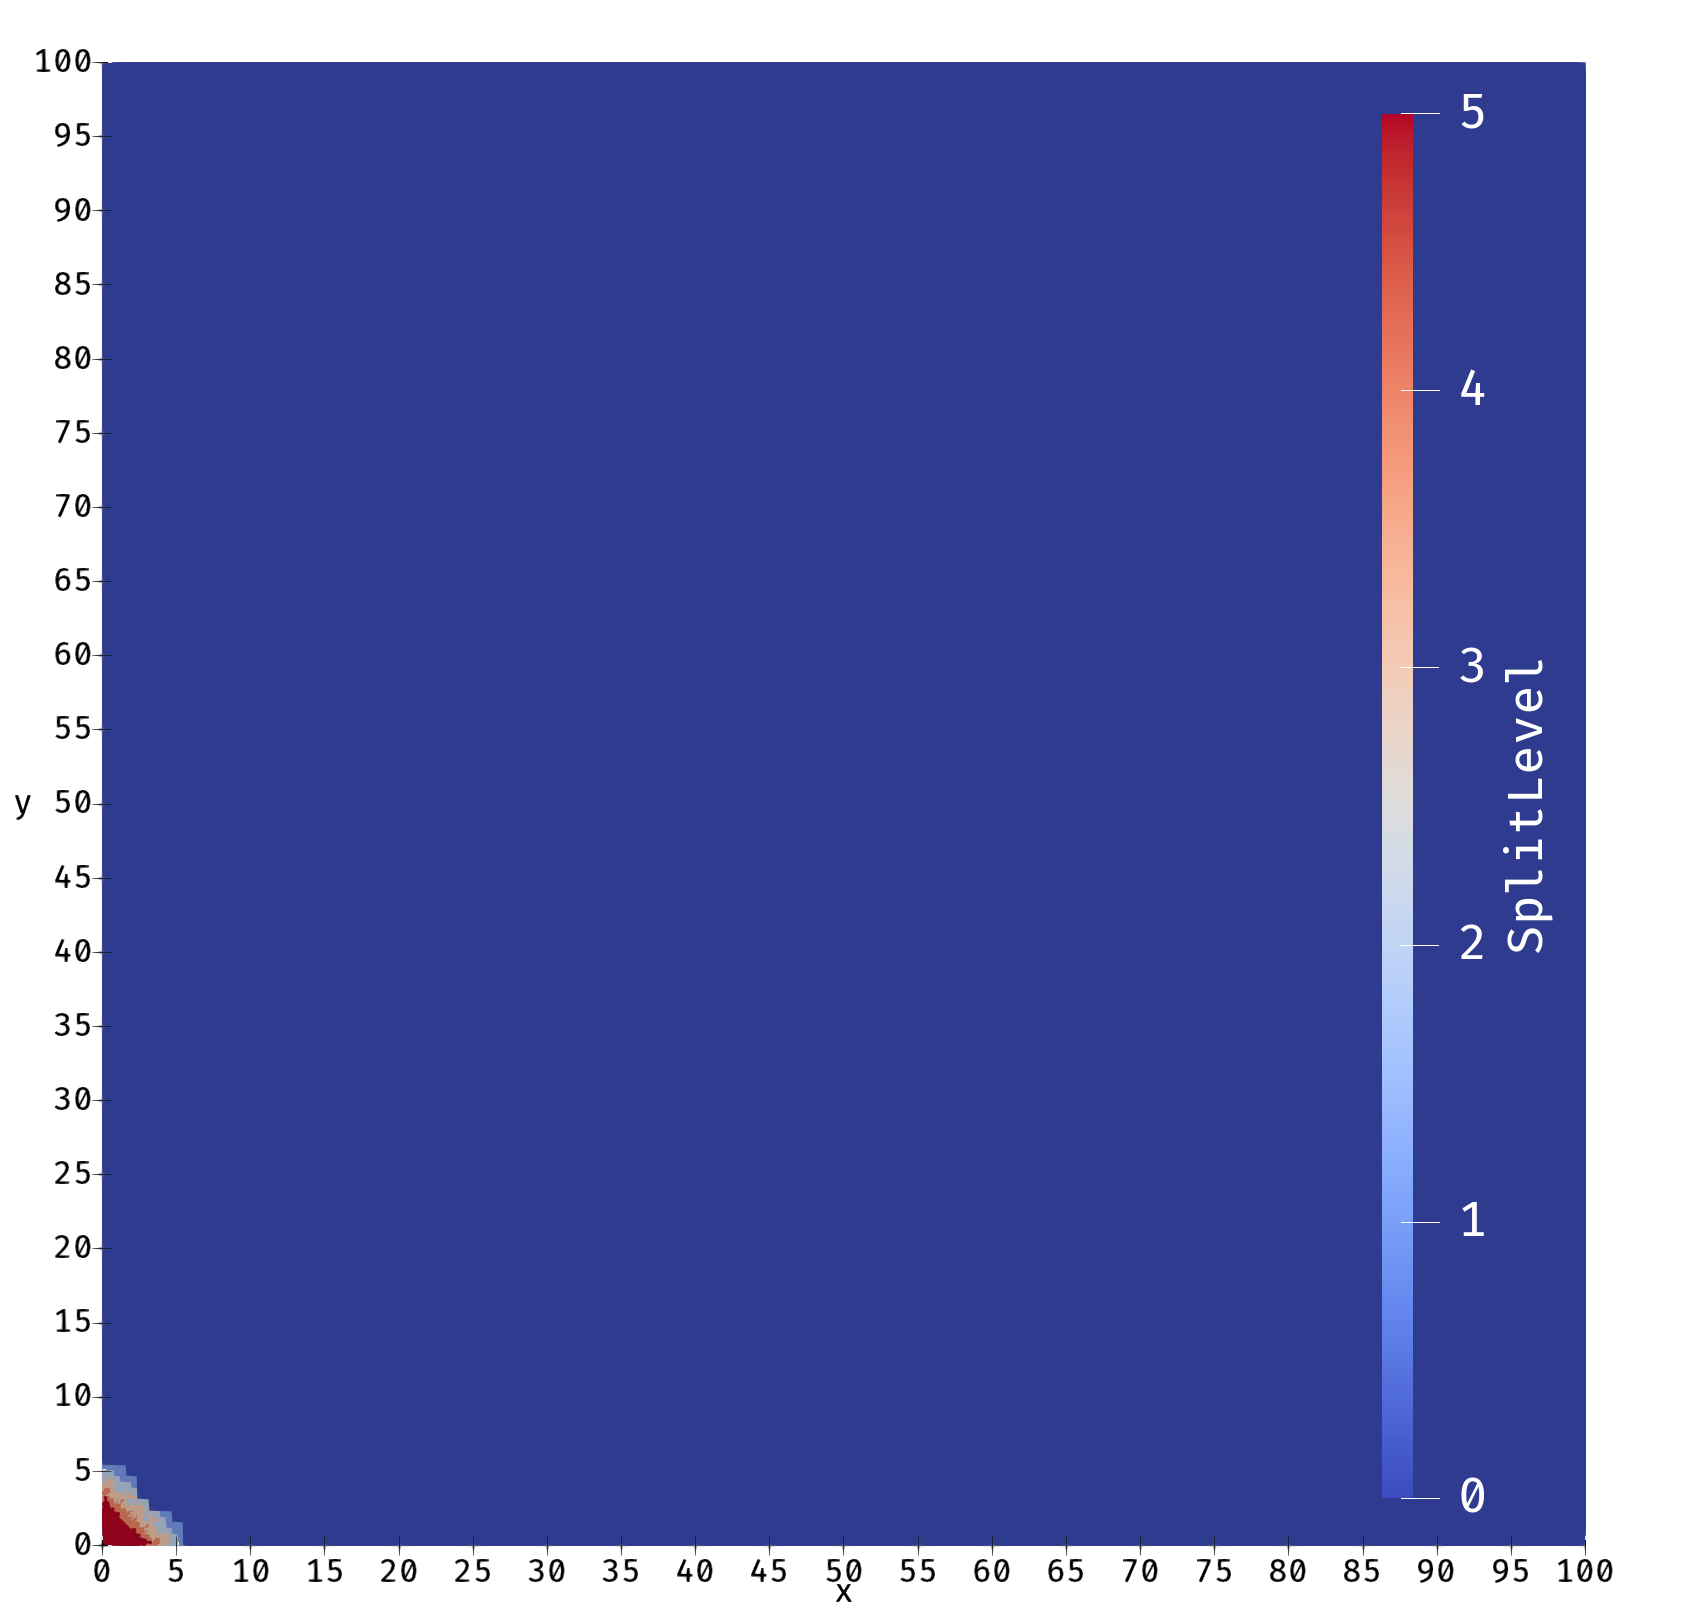
\includegraphics[width=0.5\textwidth]{Chapter_results/media/split_level_medium_far}\label{fig:load_imbalance_case_s_far}}
    \hfill
    \subfloat[Detail]
    {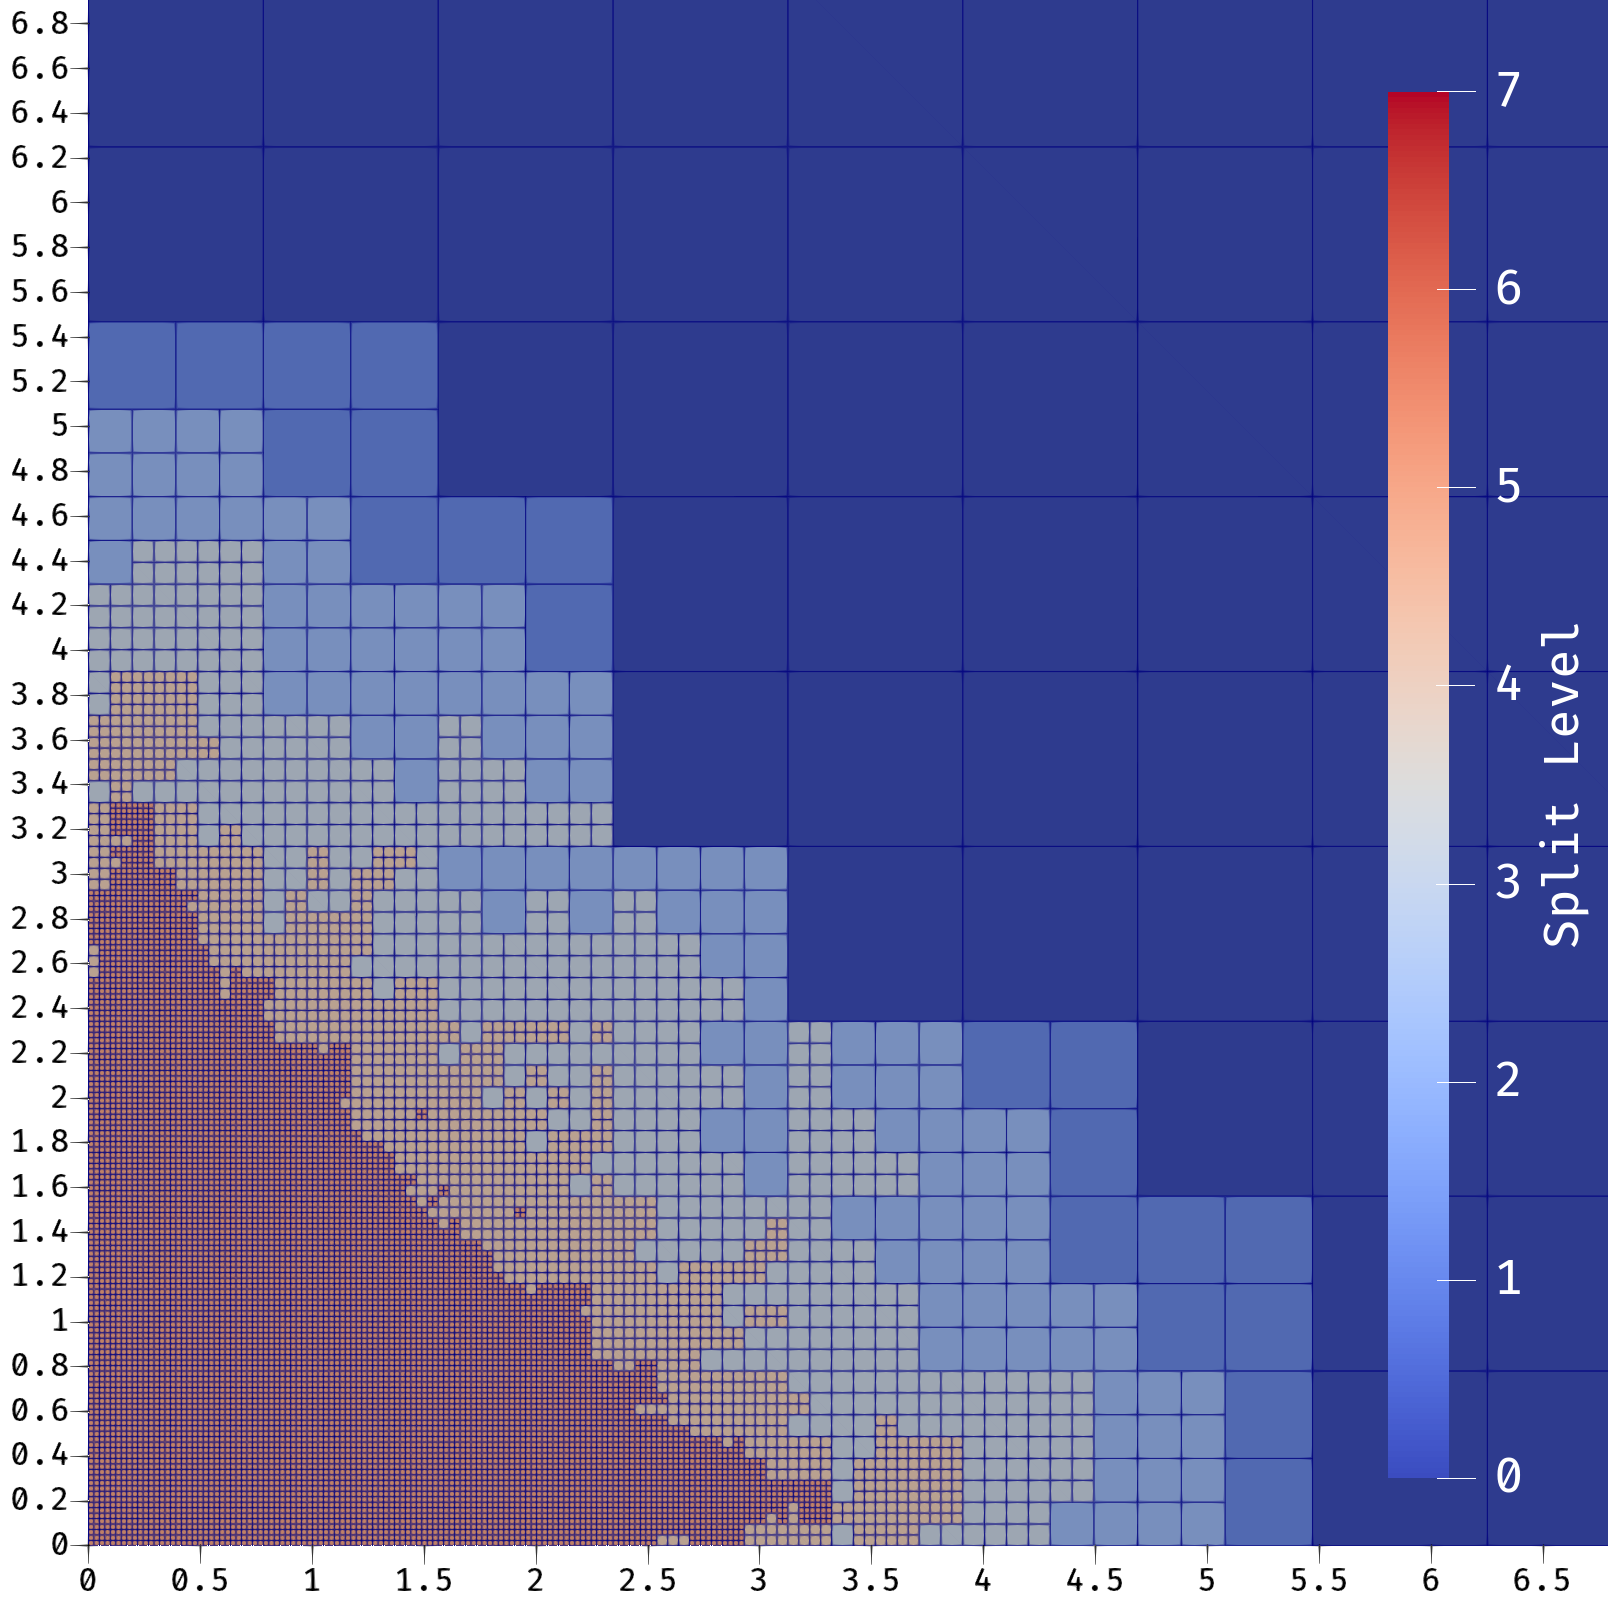
\includegraphics[width=0.48\textwidth]{Chapter_results/media/split_level_medium_near}\label{fig:load_imbalance_case_s_near}}
    \caption{Medium load imbalance (\(S = 5\)) test case split level: Split level, indicating how many times the elements have split, only the bottom left refines. \(K_{initial} = 16384\), \(K_{final} = 26734\) (a) Complete domain (b) Area of interest}\label{fig:load_imbalance_case_medium_s}
\end{figure}

\begin{figure}[H]
    \centering
    \subfloat[Full domain]
    {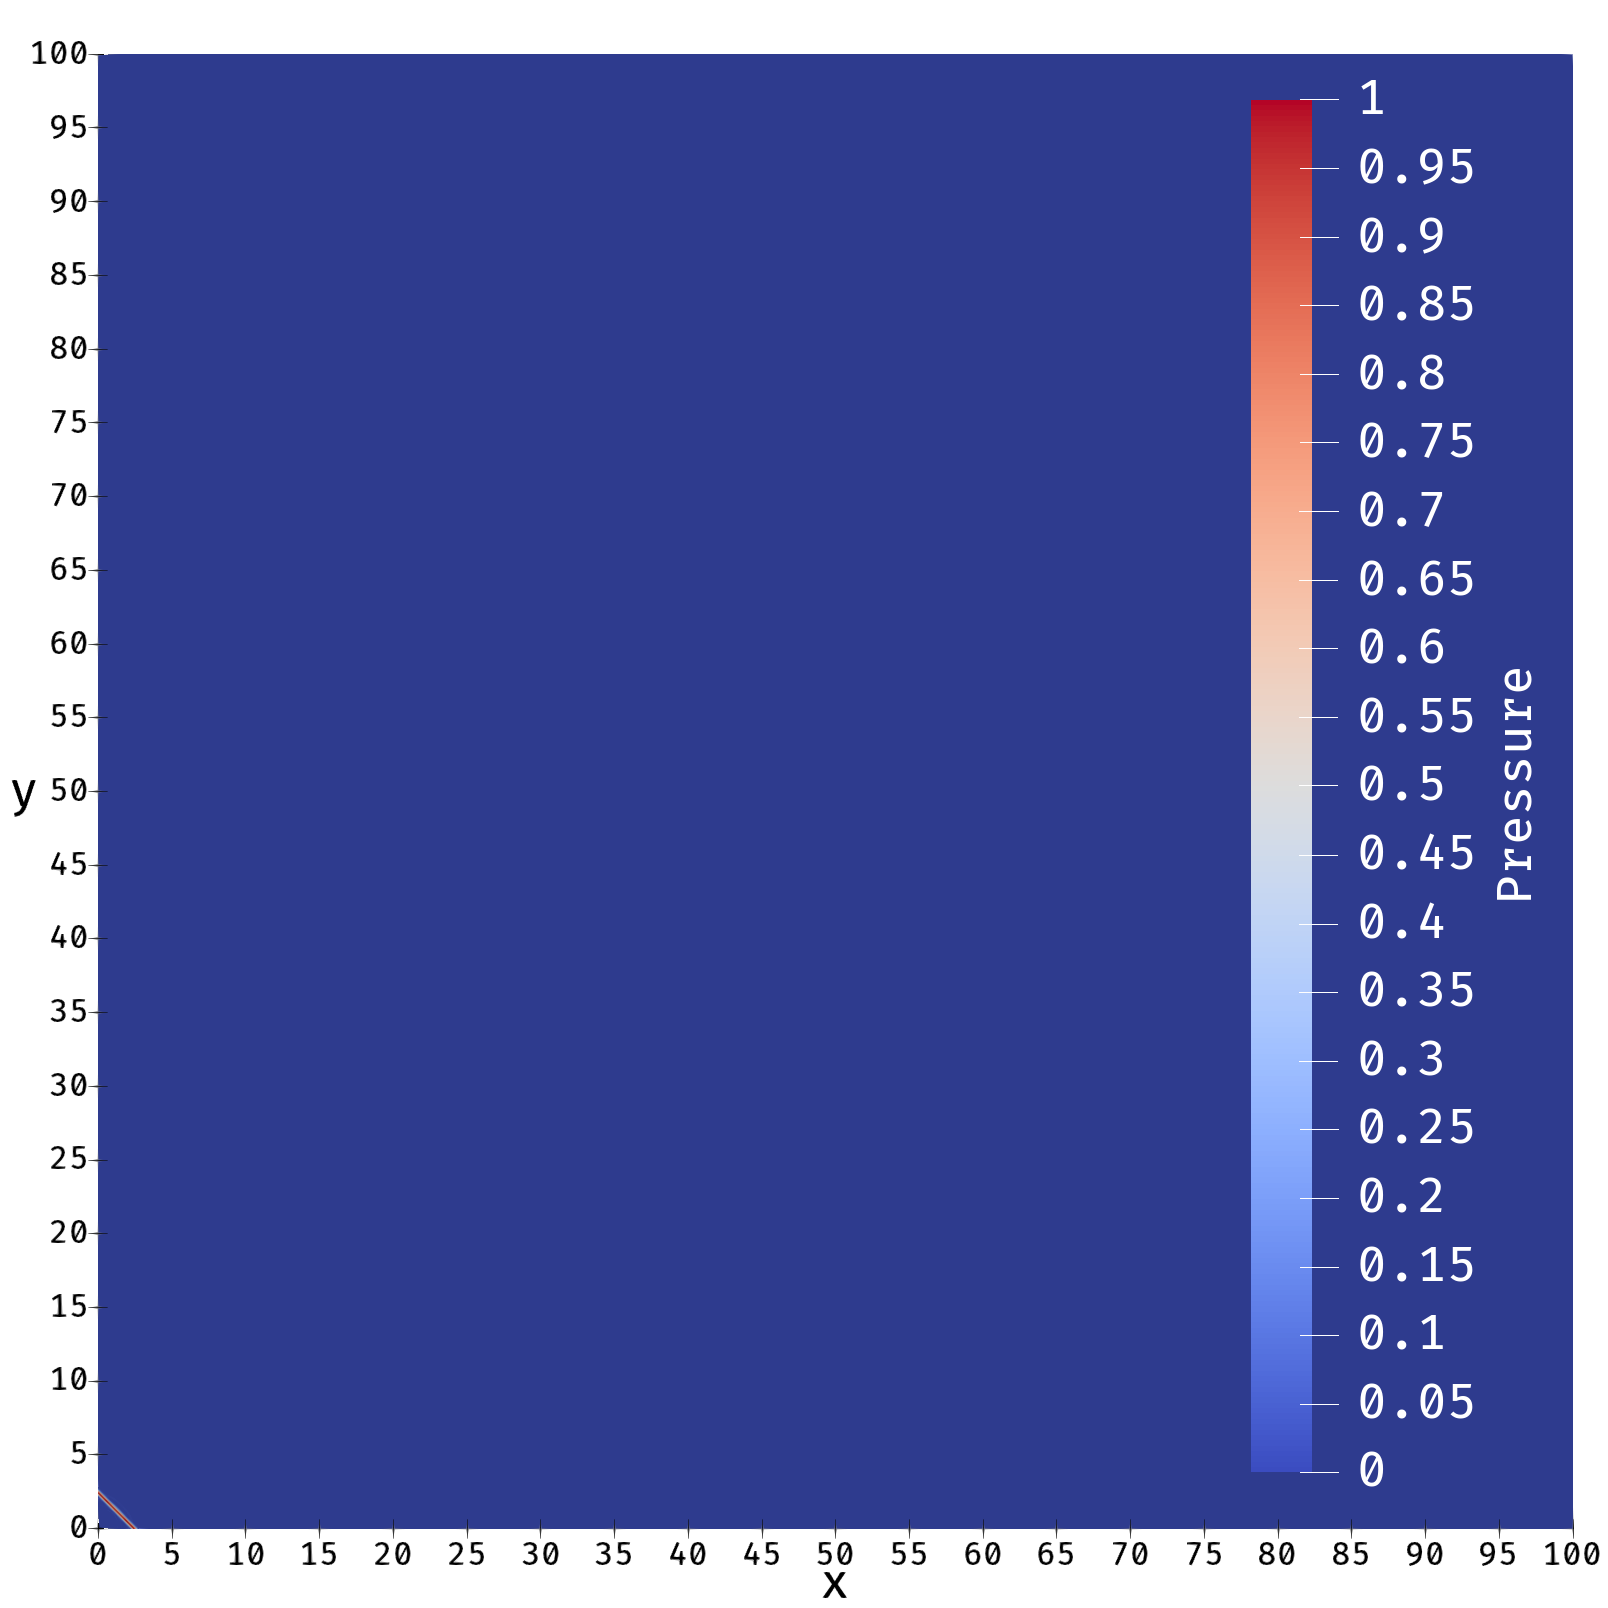
\includegraphics[width=0.5\textwidth]{Chapter_results/media/problem_high_far}\label{fig:load_imbalance_case_high_p_far}}
    \hfill
    \subfloat[Detail]
    {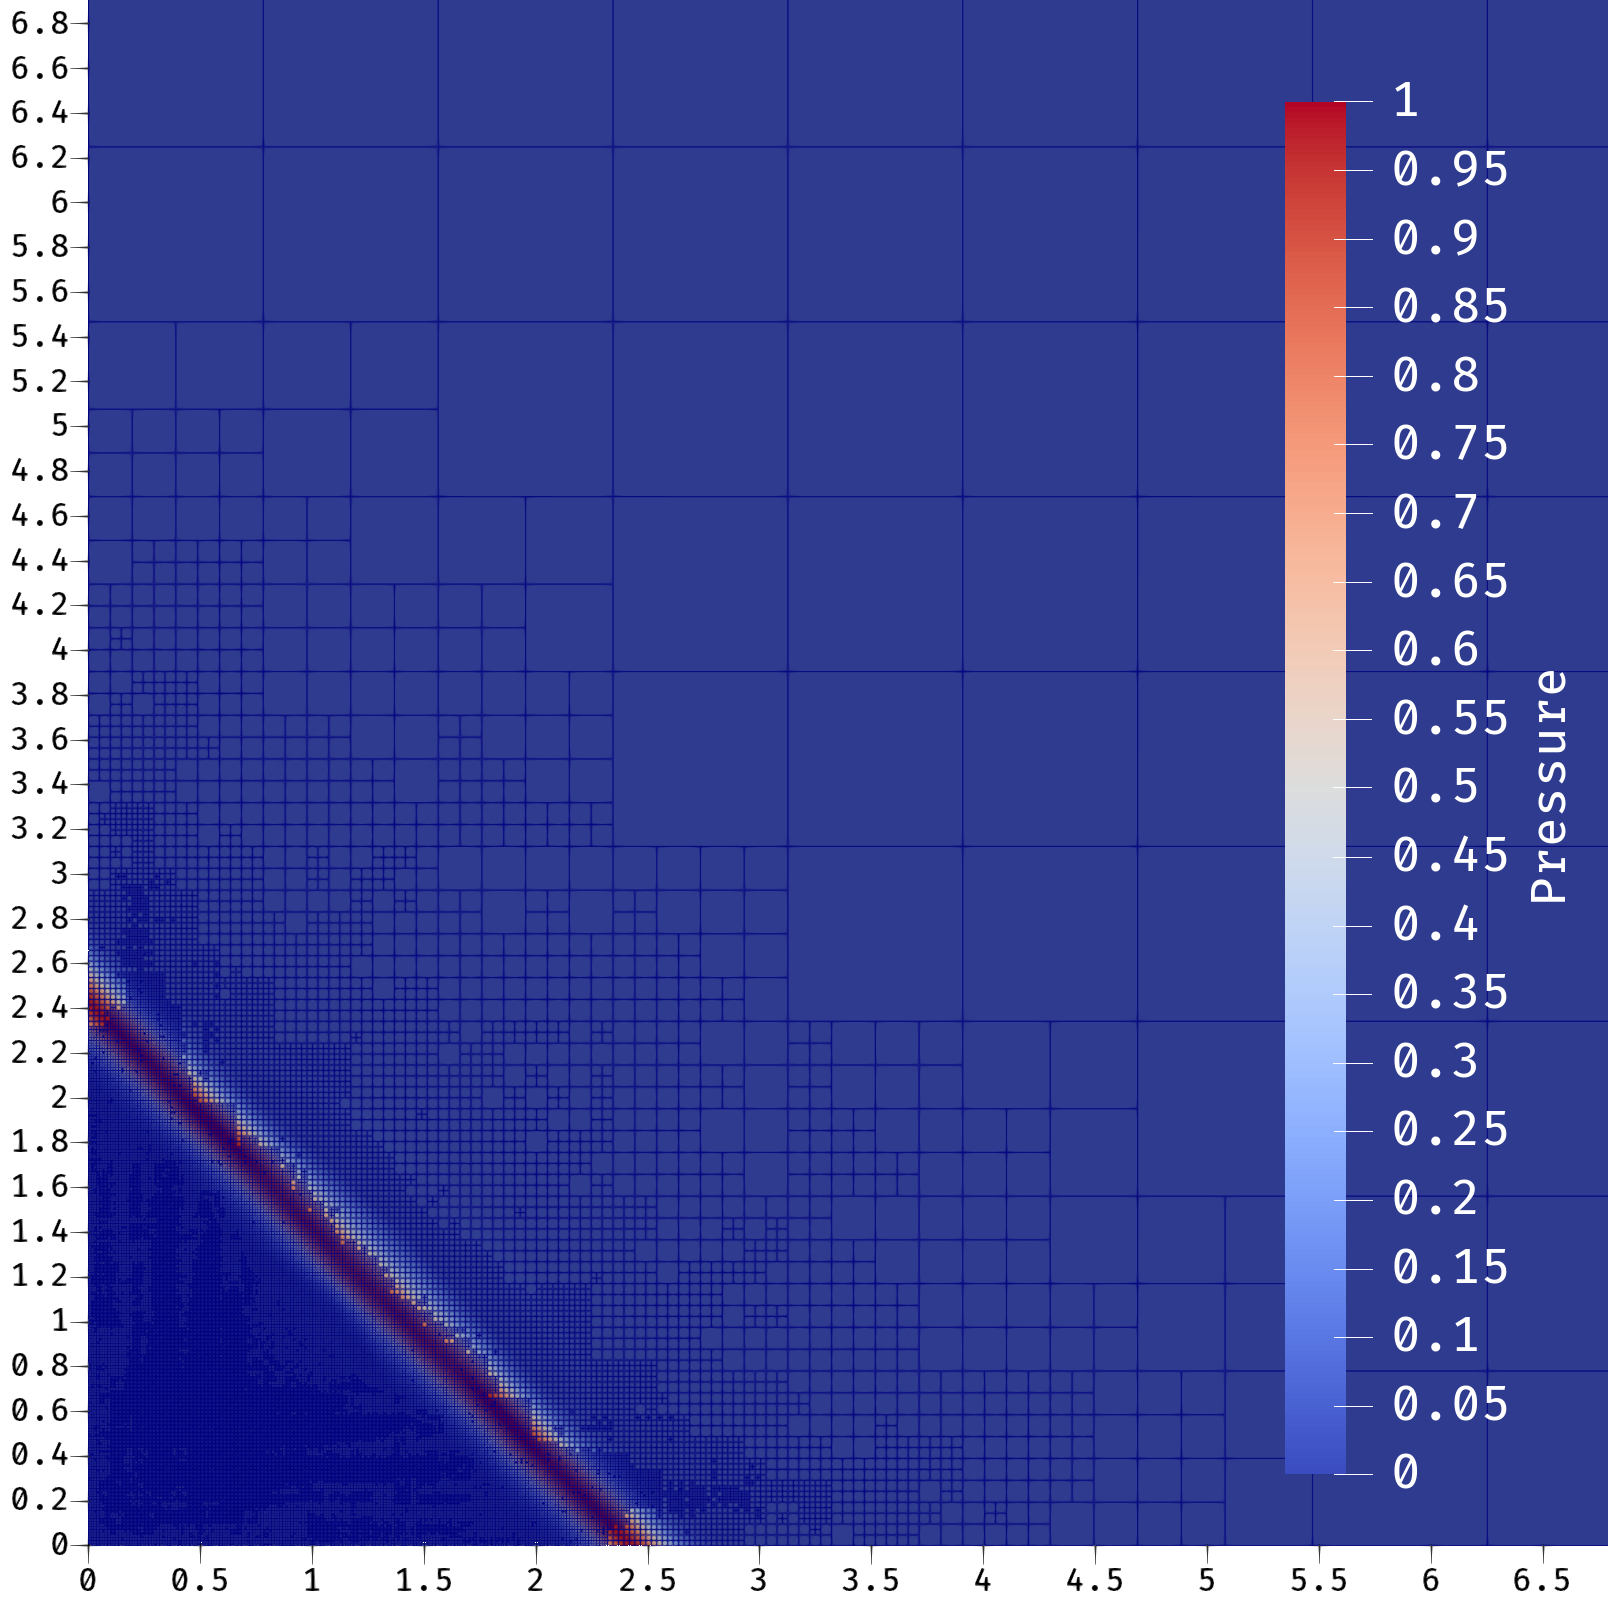
\includegraphics[width=0.48\textwidth]{Chapter_results/media/problem_high_near}\label{fig:load_imbalance_case_high_p_near}}
    \caption{High load imbalance (\(S = 7\)) test case pressure: A wave passes through a very big domain. \(K_{initial} = 16384\), \(K_{final} = 54837\) (a) Complete domain (b) Area of interest}\label{fig:load_imbalance_case_high_p}
\end{figure}

\begin{figure}[H]
    \centering
    \subfloat[Full domain]
    {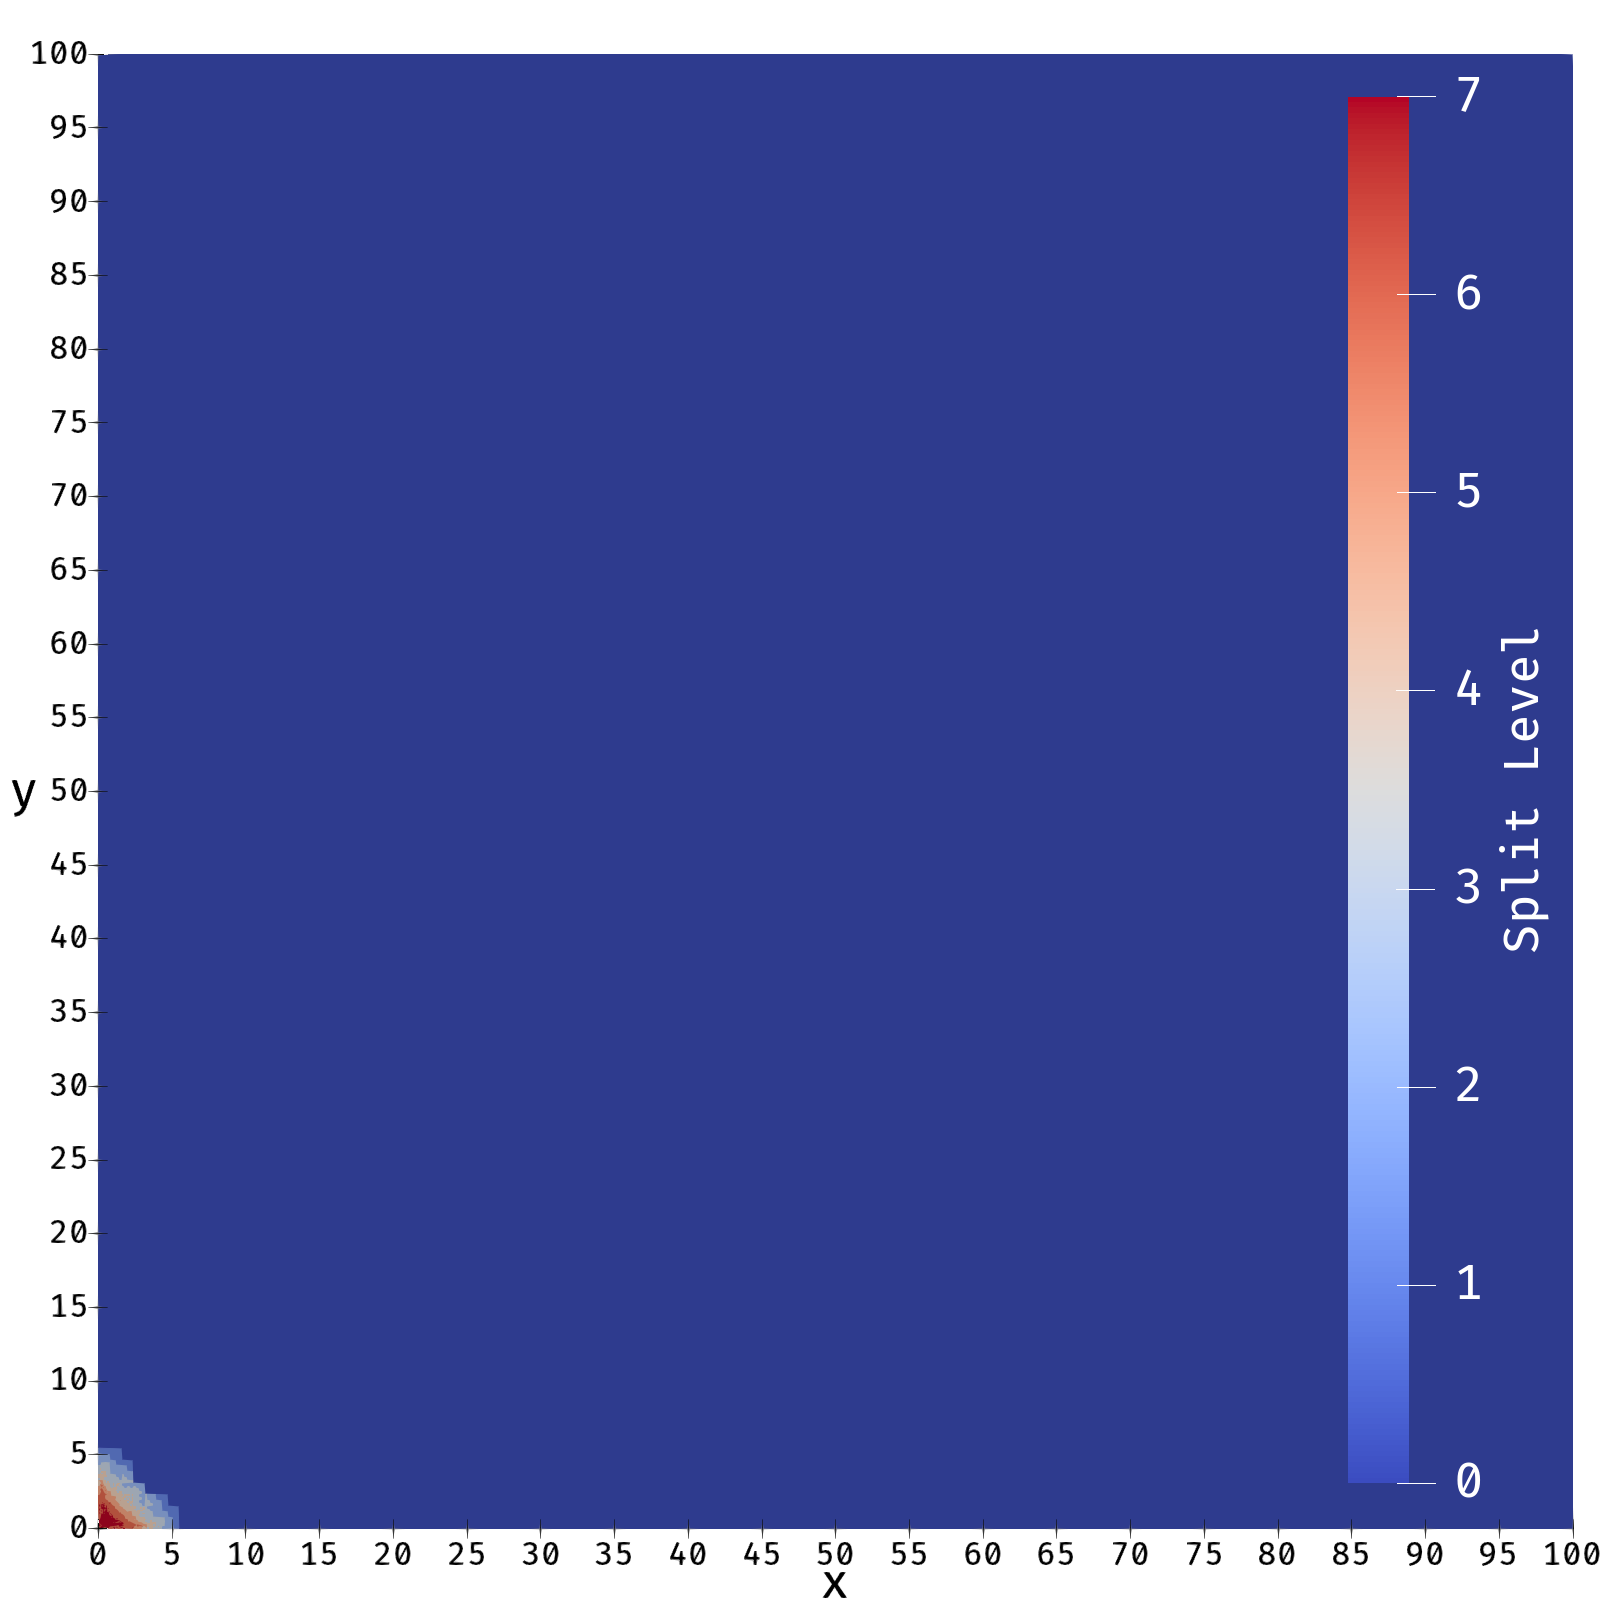
\includegraphics[width=0.5\textwidth]{Chapter_results/media/split_level_high_far}\label{fig:load_imbalance_case_high_s_far}}
    \hfill
    \subfloat[Detail]
    {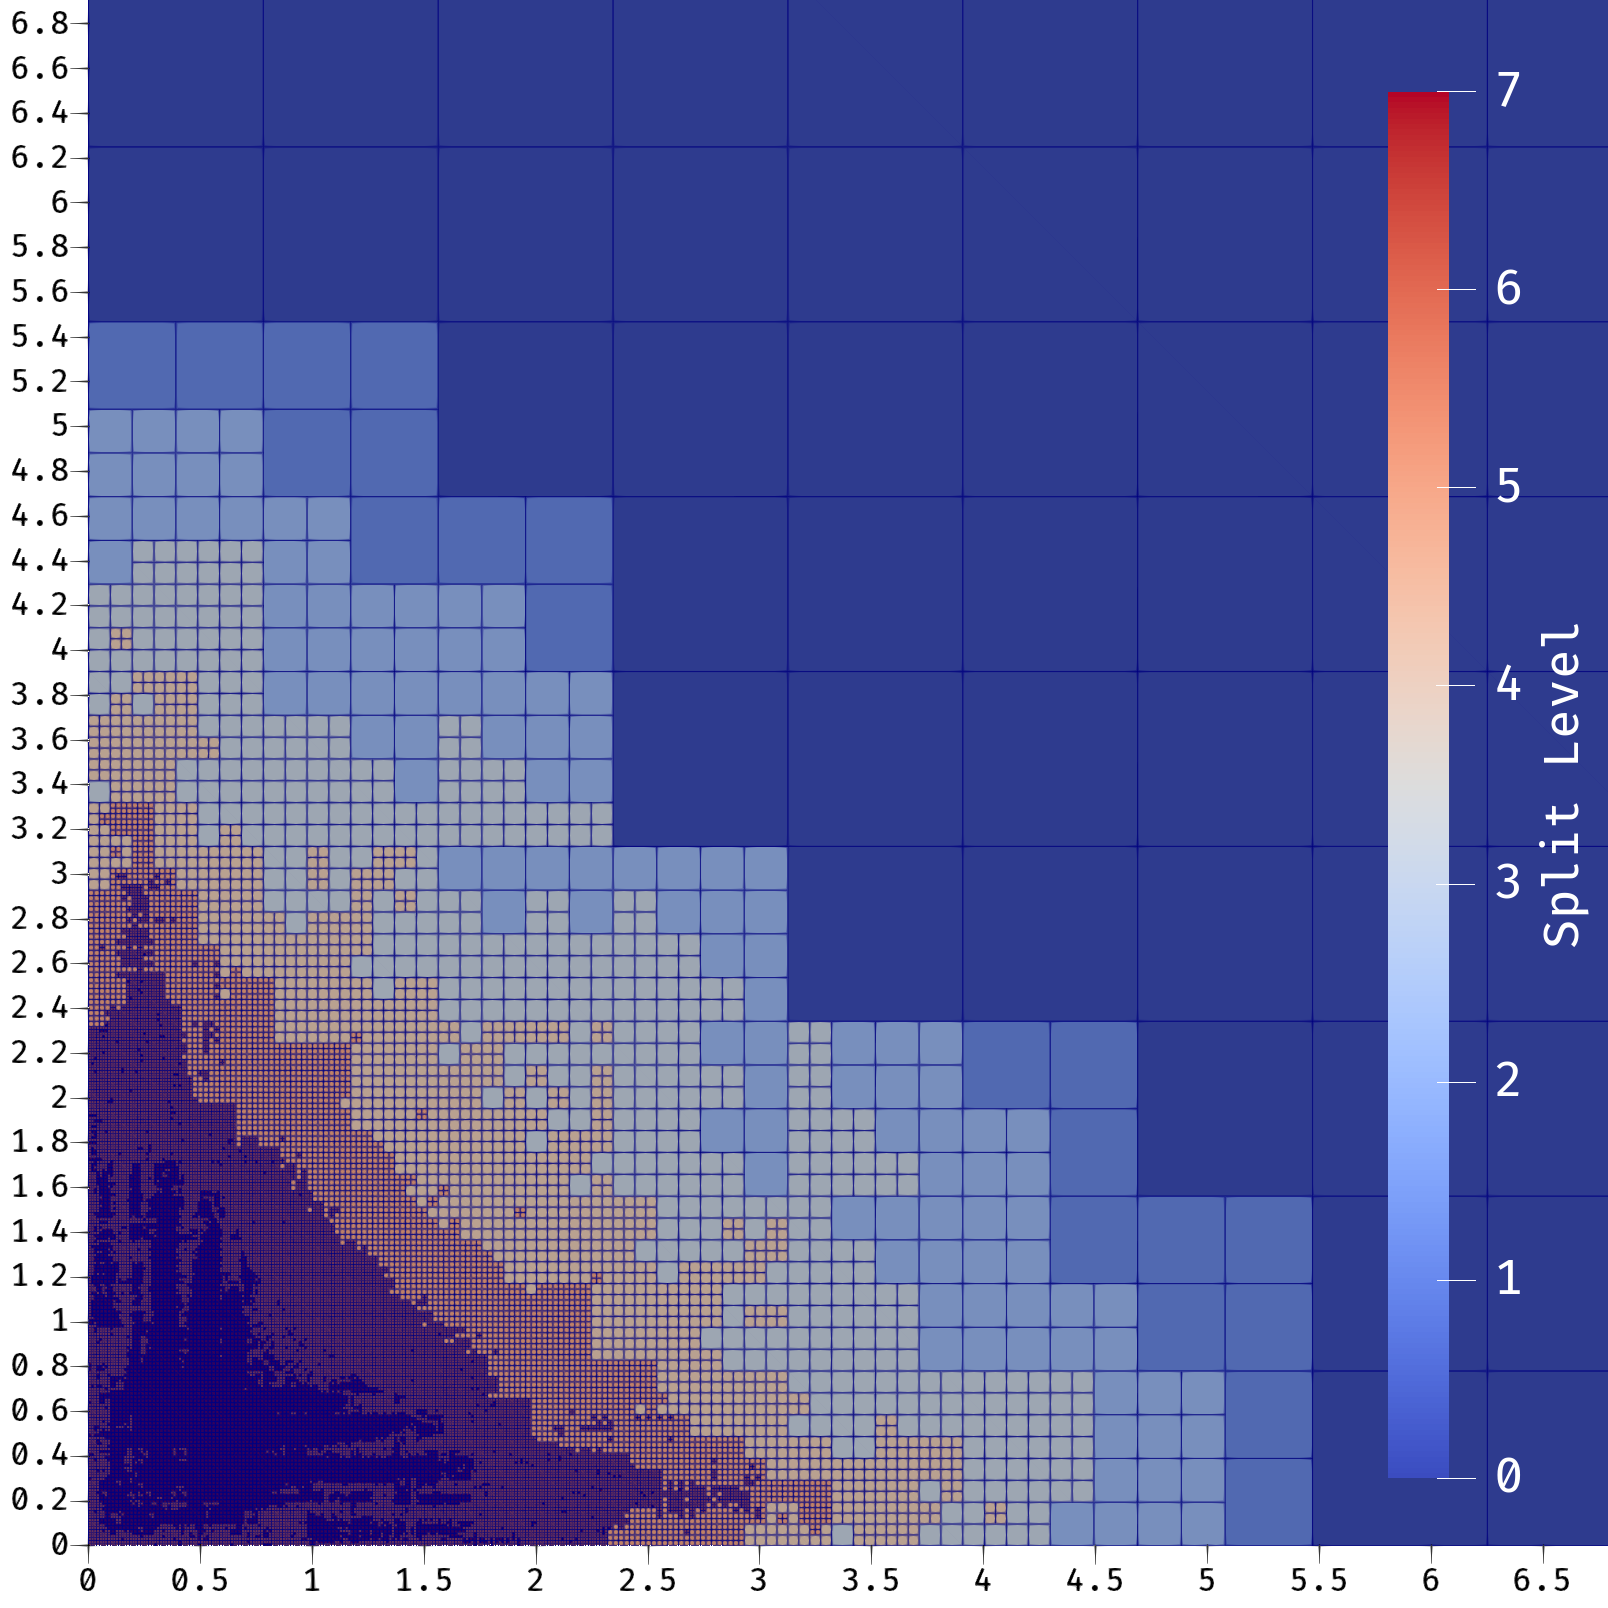
\includegraphics[width=0.48\textwidth]{Chapter_results/media/split_level_high_near}\label{fig:load_imbalance_case_high_s_near}}
    \caption{High load imbalance (\(S = 7\)) test case split level: Split level, indicating how many times the elements have split, only the bottom left refines. \(K_{initial} = 16384\), \(K_{final} = 54837\) (a) Complete domain (b) Area of interest}\label{fig:load_imbalance_case_high_s}
\end{figure}

Table~\ref{table:load_imbalance} describes the load imbalance of the three cases. \(S\) is the
maximum number of times an element can split, \(K\) is the number of elements in the mesh, \(K_p\)
is the number of elements in process \(p\), \(w_{ideal}\) is the number of elements in a process if
evenly distributed, and \(L\) is the load imbalance as described in
Equation~\ref{equ:load_imbalance}.

\begin{table}[H]
    \centering
    \begin{tabular}{ c c c c c c c }
        Case & S & K & Max \(K_p\) & \(w_{ideal}\) & \(L\) \\
        \midrule
        Low & \(3\) & \(17752\) & \(2392\) & \(1110\) & \(2.16\) \\
        Medium & \(5\) & \(26734\) & \(11374\) & \(1671\) & \(6.81\) \\
        High & \(7\) & \(62490\) & \(47130\) & \(3906\) & \(12.07\) \\
    \end{tabular}
    \caption{Load imbalance cases.}\label{table:load_imbalance}
\end{table}

We compare two approaches to choose when to load balance the mesh, as described in
Section~\ref{section:load_balancing:criteria}. We compare the three cases above with and without
load balancing.

\subsection{Load balancing interval}\label{subsection:results:load_balancing_performance:interval}

We start by varying the load balancing interval for the three cases in
Figures~\ref{fig:load_balancing_efficiency_interval_s3},~\ref{fig:load_balancing_efficiency_interval_s5}
and~\ref{fig:load_balancing_efficiency_interval_s7}. Since we refine the mesh every 20 time steps, a
load balancing interval of 20 is equivalent to load balancing the mesh every time we refine it, up
to every 50 times we refine for a load balancing interval of 1000. The dashed line represents the
performance without load balancing.

\begin{figure}[H]
    \begin{adjustwidth}{-0.5in}{-0.5in}
    \centering
    \subfloat[Low load imbalance]
    {\includesvg[width=0.39\textwidth]{Chapter_results/media/load_balancing_interval_N4_K16384_A20_P16_S3}\label{fig:load_balancing_efficiency_interval_s3}}
    \hfill
    \subfloat[Medium load imbalance]
    {\includesvg[width=0.39\textwidth]{Chapter_results/media/load_balancing_interval_N4_K16384_A20_P16_S5}\label{fig:load_balancing_efficiency_interval_s5}}
    \hfill
    \subfloat[High load imbalance]
    {\includesvg[width=0.39\textwidth]{Chapter_results/media/load_balancing_interval_N4_K16384_A20_P16_S7}\label{fig:load_balancing_efficiency_interval_s7}}
    \end{adjustwidth}
    \caption{Load balancing performance interval test: Simulation time with refinement and load balancing while increasing load balancing interval. \(N_{initial} = 4\), \(K_{initial} = 16384\), refinement interval = 20, \(P = 16\) (a) \(S = 3\) (b) \(S = 5\) (c) \(S = 7\)}\label{fig:load_balancing_efficiency_interval}
\end{figure}

From Figure~\ref{fig:load_balancing_efficiency_interval}, we see that load balancing diminishes the
computation time of all three problems. The low load imbalance case needs a higher load balancing
interval to offset the cost of the load balancing algorithm. In the other cases, the load imbalance
is great enough that the cases with load balancing are always faster. It takes a certain load
balancing interval to obtain the best performance, and that interval changes with the case. Next, we
will study an alternative algorithm to improve on those two points.

\subsection{Load balancing threshold}\label{subsection:results:load_balancing_performance:threshold}

We now use an allowable load imbalance threshold to choose when to perform load balancing, as
described in Section~\ref{section:load_balancing:criteria}. This means we assess the load imbalance
\(L\) of the mesh after each refinement step, and we only perform load balancing if it is above a
certain threshold. We start with a threshold of \(1\), equivalent to load balancing after every
refinement step, to \(2\), equivalent to load balancing only if a \acrshort{acr:GPU} has two or more
times the workload it would have if the mesh was perfectly balanced. The same three load imbalance
cases from Section~\ref{section:results:load_balancing_performance} are shown in
Figure~\ref{fig:load_balancing_efficiency_threshold}.

\begin{figure}[H]
    \begin{adjustwidth}{-0.5in}{-0.5in}
    \centering
    \subfloat[Low load imbalance]
    {\includesvg[width=0.39\textwidth]{Chapter_results/media/load_balancing_threshold_N4_K16384_A20_L20_P16_S3}\label{fig:load_balancing_efficiency_threshold_s3}}
    \hfill
    \subfloat[Medium load imbalance]
    {\includesvg[width=0.39\textwidth]{Chapter_results/media/load_balancing_threshold_N4_K16384_A20_L20_P16_S5}\label{fig:load_balancing_efficiency_threshold_s5}}
    \hfill
    \subfloat[High load imbalance]
    {\includesvg[width=0.39\textwidth]{Chapter_results/media/load_balancing_threshold_N4_K16384_A20_L20_P16_S7}\label{fig:load_balancing_efficiency_threshold_s7}}
    \end{adjustwidth}
    \caption{Load balancing performance threshold test: Simulation time with refinement and load balancing while increasing load balancing threshold. \(N_{initial} = 4\), \(K_{initial} = 16384\), refinement interval = 20, load balancing interval = 20, \(P = 16\) (a) \(S = 3\) (b) \(S = 5\) (c) \(S = 7\)}\label{fig:load_balancing_efficiency_threshold}    
\end{figure}

From Figure~\ref{fig:load_balancing_efficiency_threshold}, we observe that using a load imbalance
threshold to control when we load balance is a much better solution than simply increasing the
interval at which we perform load balancing. The performance improves quickly when increasing the
threshold, and the threshold values that work well do not seem to change with the problem. A load
imbalance threshold of around \(1.1\) seems to give good performance in all cases, and would not
need to be adapted to different cases.

\subsection{Overall load balancing performance}\label{subsection:results:load_balancing_performance:overall}

From the results of Subsections~\ref{subsection:results:load_balancing_performance:interval}
and~\ref{subsection:results:load_balancing_performance:threshold}, we observe that load balancing at
every occasion incurs a significant performance penality, sometimes performing worse than the non
load-balanced case in the low load imbalance case, in
Figures~\ref{fig:load_balancing_efficiency_interval_s3}
and~\ref{fig:load_balancing_efficiency_threshold_s3}. The two other cases also show worse
performance with a low load balancing interval or load imbalance threshold. This is because the
dynamic load balancing process is expensive, especially since we are using \acrshortpl{acr:GPU},
because of the numerous data transfers and memory allocations performed. We must choose judiciously
our load balancing strategy. 

The performance increases as we space out load balancing, either by increasing the load balancing
interval, or by increasing the load imbalance threshold, up to a point. Past that point, an interval
of \(500\) or a threshold of \(1.5\) in this case, the performance goes down due to the mesh being
more imbalanced for longer periods of time.

The load imbalance threshold strategy from
Subsection~\ref{subsection:results:load_balancing_performance:threshold} gives better results, the
performance improves quickly when increasing the threshold and stays high longer than the load
balancing interval strategy from
Subsection~\ref{subsection:results:load_balancing_performance:interval}. The load balancing interval
is also case dependent, and must be adjusted according to the scale of the problem and how often it
is refined. 

For these reasons we choose the load imbalance threshold strategy with a load imbalance threshold of
\(1.1\) to assess the overall dynamic load balancing performance in
Figure~\ref{fig:load_balancing_efficiency}. It shows the speedup we get from load balancing the
three problems. The \(x\) axis represents the equivalent load imbalance \(L\) of the problems if
they were not load balanced.

\begin{figure}[H]
    \centering
    \includesvg[width=0.6\textwidth]{Chapter_results/media/load_balancing_threshold_N4_K16384_A20_L20_P16_T1.1}
    \caption{Load balancing performance: Simulation time with refinement and load balancing while increasing load imbalance. \(N_{initial} = 4\), \(K_{initial} = 16384\), refinement interval = 20, load balancing interval = 20, \(P = 16\), load balancing threshold = \(1.1\)}\label{fig:load_balancing_efficiency}
\end{figure}

Figure~\ref{fig:load_balancing_efficiency} shows that dynamic load balancing performs well, and is
able to regain performance lost to load imbalance. In the high load imbalance case, with a load
imbalance of \(L = 12.07\), dynamic load balancing can improve performance by \(4.1 \times \). It
scales well with load imbalance, meaning it gives good results no matter the level of imbalance of
the problem. The gains are especially crucial for high imbalance levels, where the load imbalance
can degrade performance by an order of magnitude. In these cases, dynamic load balancing can regain
most of the lost performance.

\subsection{Polynomial order influence}\label{subsection:results:load_balancing_performance:polynomial_order}

Figure~\ref{fig:N_influence} shows a comparison of the iteration time as a function of the
polynomial order \(N\) of a uniformly refined mesh, both on the \acrshort{acr:CPU} and
\acrshort{acr:GPU}. This shows how computing time scales on the two types of processors with
increasing \(N\), and could guide how elements should be weighted individually when performing load
balancing, instead of being all weighted equally as they are in this work. The test case was
computed using the Narval supercomputer, using a grid with \(64\) elements in each of the the \(x\)
and \(y\) directions. The initial polynomial order of the mesh is indicated on the \(y\) axis, and
the problem is advanced by \(1000\) iterations in all cases. \Acrshort{acr:AMR} is performed every
\(100\) iterations, but there are enough elements that the mesh never refines, it only estimates the
error. The \acrshort{acr:CPU} case is computed on a single \acrshort{acr:CPU} core, and the
\acrshort{acr:GPU} case is computed on a single \acrshort{acr:GPU}.

\begin{figure}[H]
    \centering
    \subfloat[\Acrshort{acr:CPU} and \Acrshort{acr:GPU}]
    {\includesvg[width=0.5\textwidth]{Chapter_results/media/N_cpu_iteration_time}\label{fig:N_cpu_influence}}
    \hfill
    \subfloat[\Acrshort{acr:GPU} detail]
    {\includesvg[width=0.48\textwidth]{Chapter_results/media/N_gpu_iteration_time}\label{fig:N_gpu_influence}}
    \caption{Polynomial order influence: Iteration time with increasing polynomial order \(N\). (a)
        \Acrshort{acr:CPU} and \Acrshort{acr:GPU}. (b) \Acrshort{acr:GPU} detail, emphasising the 
        slope.}\label{fig:N_influence}
\end{figure}

Figure~\ref{fig:N_influence} shows that the relation between iteration time and polynomial order
\(N\) on the \acrshort{acr:GPU} is closer to being linear in this range. This is unexpected, as we
expect the relation between polynomial order and computing time to scale with \({\left( N + 1
\right)}^3\) like on the \acrshort{acr:CPU}, as the number of operations to perform on every time
step scales with \({\left( N + 1 \right)}^3\). This may be explained by the fact that
\acrshortpl{acr:GPU} favour more arithmetically intense computations. As \(N\) increases, there are
more compute operations to perform relative to other operations like scheduling and launching
kernels, which may increase the workload of \acrshortpl{acr:GPU} and increase their performance. An
increase in realisable \acrshort{acr:GPU} performance in GFLOPS has been observed when \(N\)
increases, as for example by Chan et al.~\cite{Chan2016}.

\section{Complex Case}\label{section:results:complex_application}

We now present a more complex case with all modules of the program enabled. Figure~\ref{fig:cloud_p}
shows the pressure distribution at two times. The problem depicts a diagonal wave moving through a
small circular ``cloud'' of higher pressure. The cloud expands and interacts with the wave. The mesh
is initially split into \(16\) elements in each of the \(x\) and \(y\) directions, for a total of
\(K = 256\) elements. The polynomial order of the elements is initially \(N = 4\). The solution is
computed in parallel on \(16\) \acrshortpl{acr:GPU}. The mesh is refined every \(50\) timesteps, and
load balanced with an imbalance threshold of \(L = 1.1\). It is allowed to refine up to \(S = 3\)
and \(N = 16\). Three steps of mesh pre-condition are performed, which is why the \(t = 0 s\) mesh
is already refined in Figures~\ref{fig:cloud_s_t0} and~\ref{fig:cloud_N_t0}.
Figure~\ref{fig:cloud_s} shows the split level \(S\) of the mesh, Figure~\ref{fig:cloud_N} the
polynomial order \(N\) of the mesh, and Figure~\ref{fig:cloud_rank} the rank of the elements. The
rank indicates which of the \(16\) \acrshortpl{acr:GPU} is responsible for which part of the mesh,
and how this changes with time as the mesh is load balanced.

\begin{figure}[H]
    \centering
    \subfloat[\( t = 0 s\)]
    {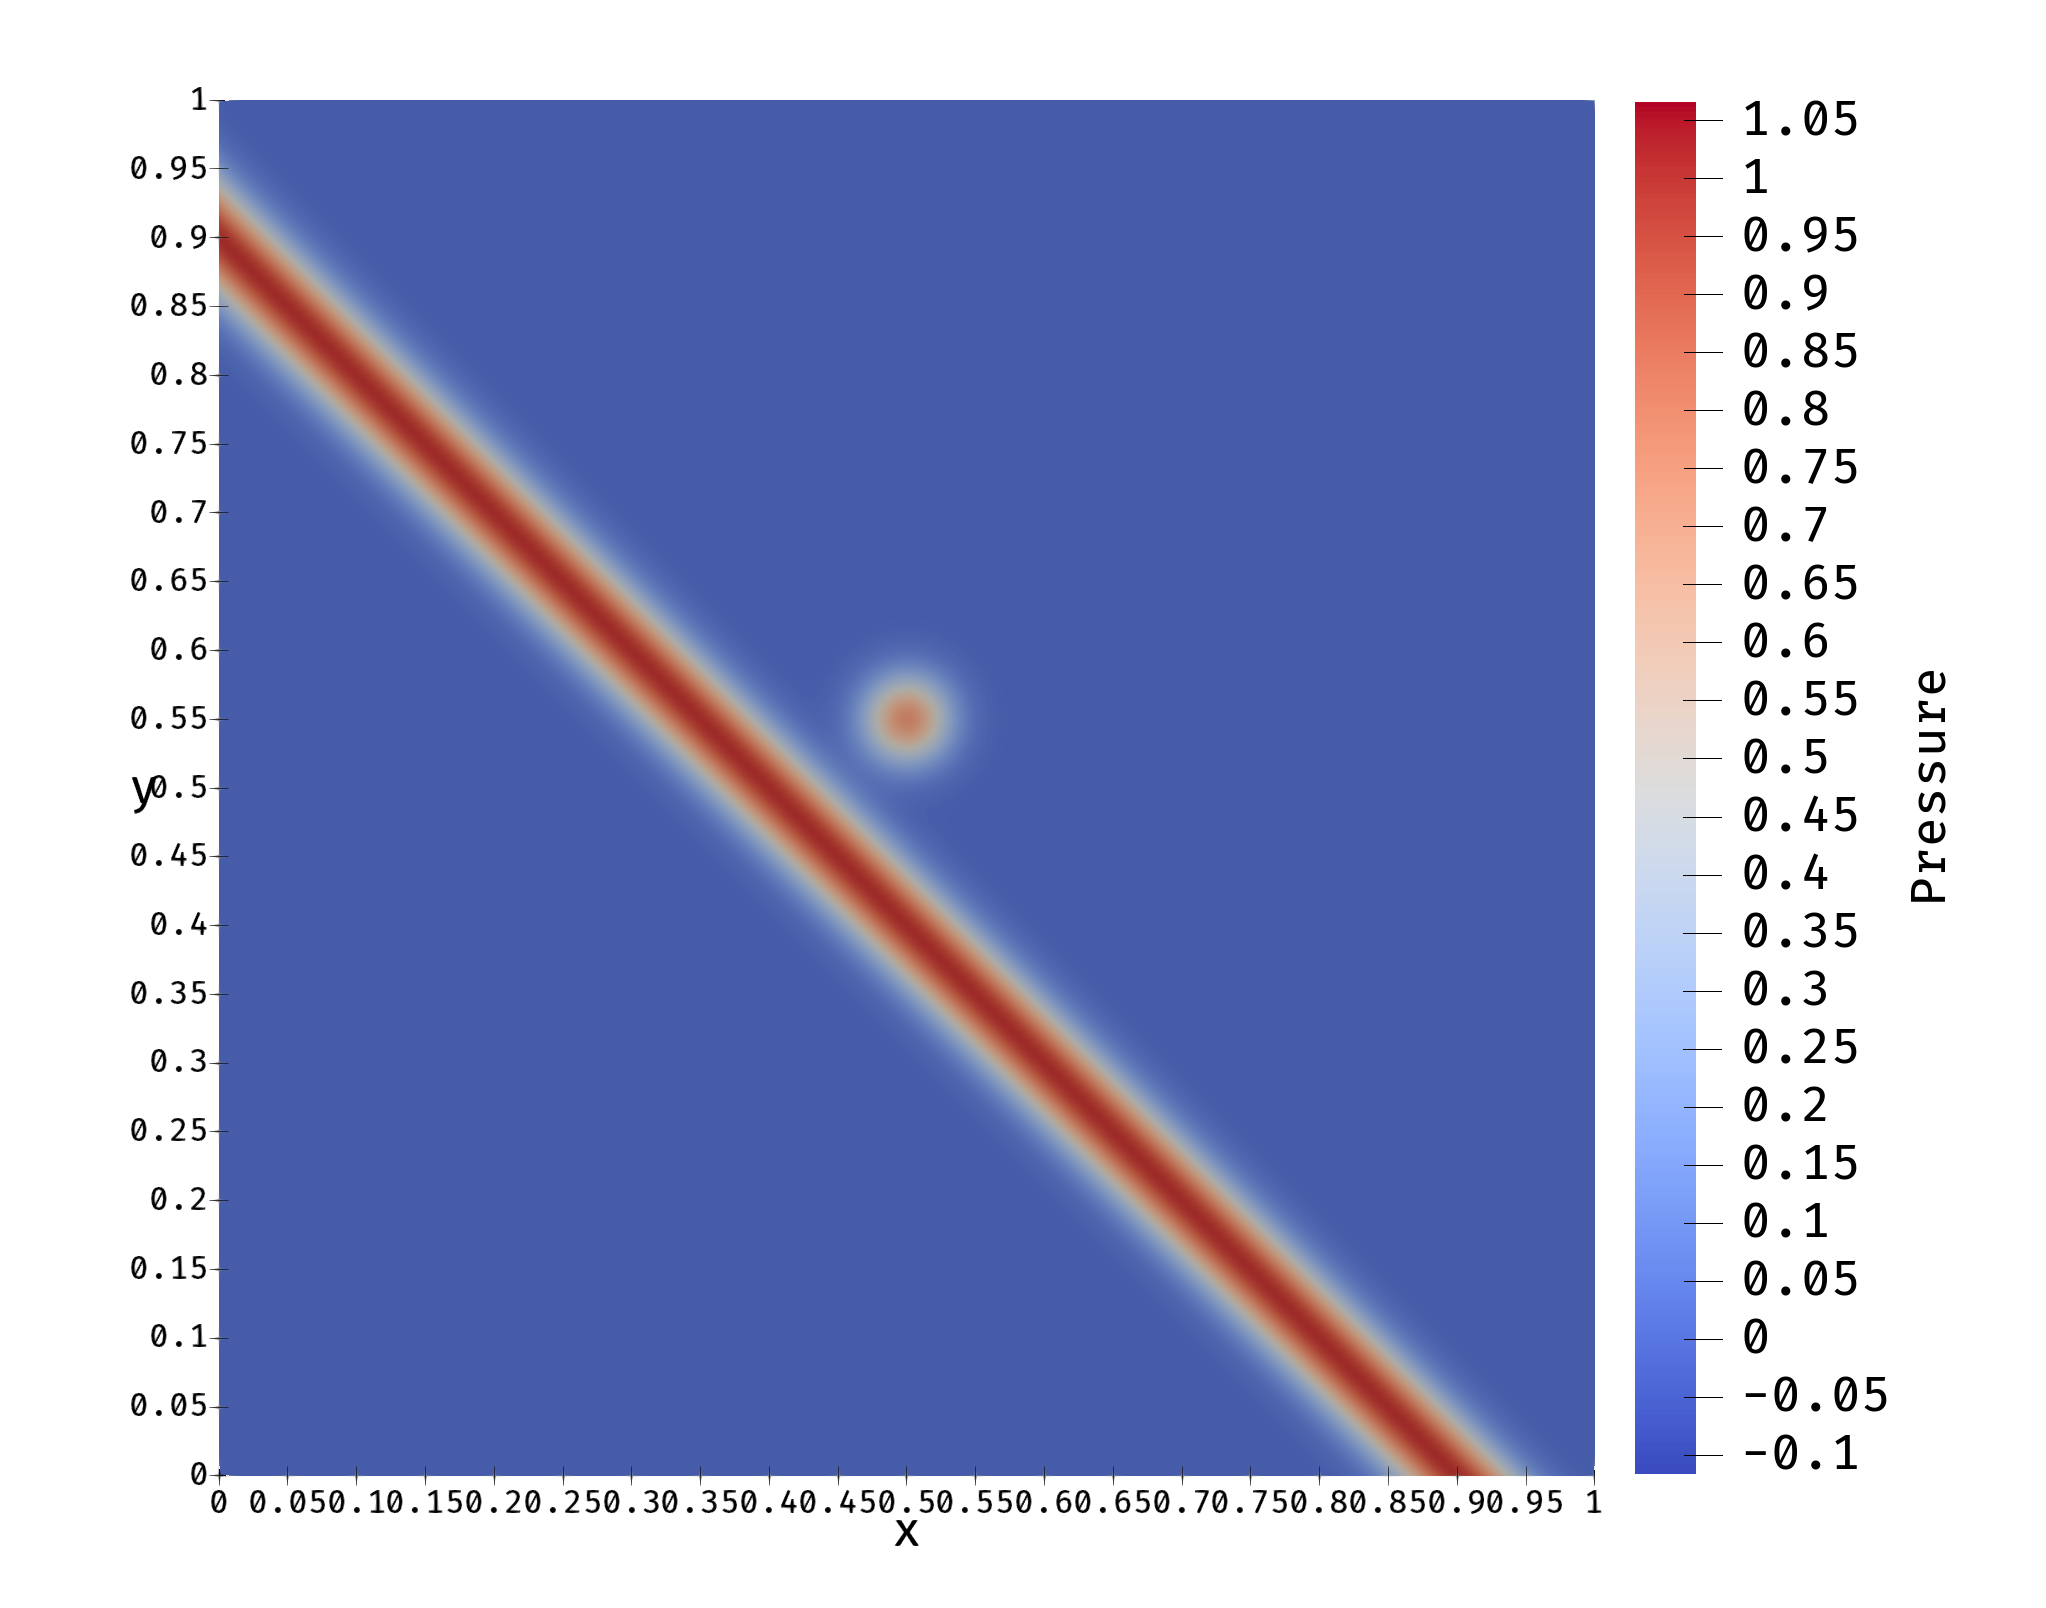
\includegraphics[width=0.48\textwidth]{Chapter_results/media/cloud_t0}\label{fig:cloud_p_t0}}
    \hfill
    \subfloat[\( t = 0.2 s\)]
    {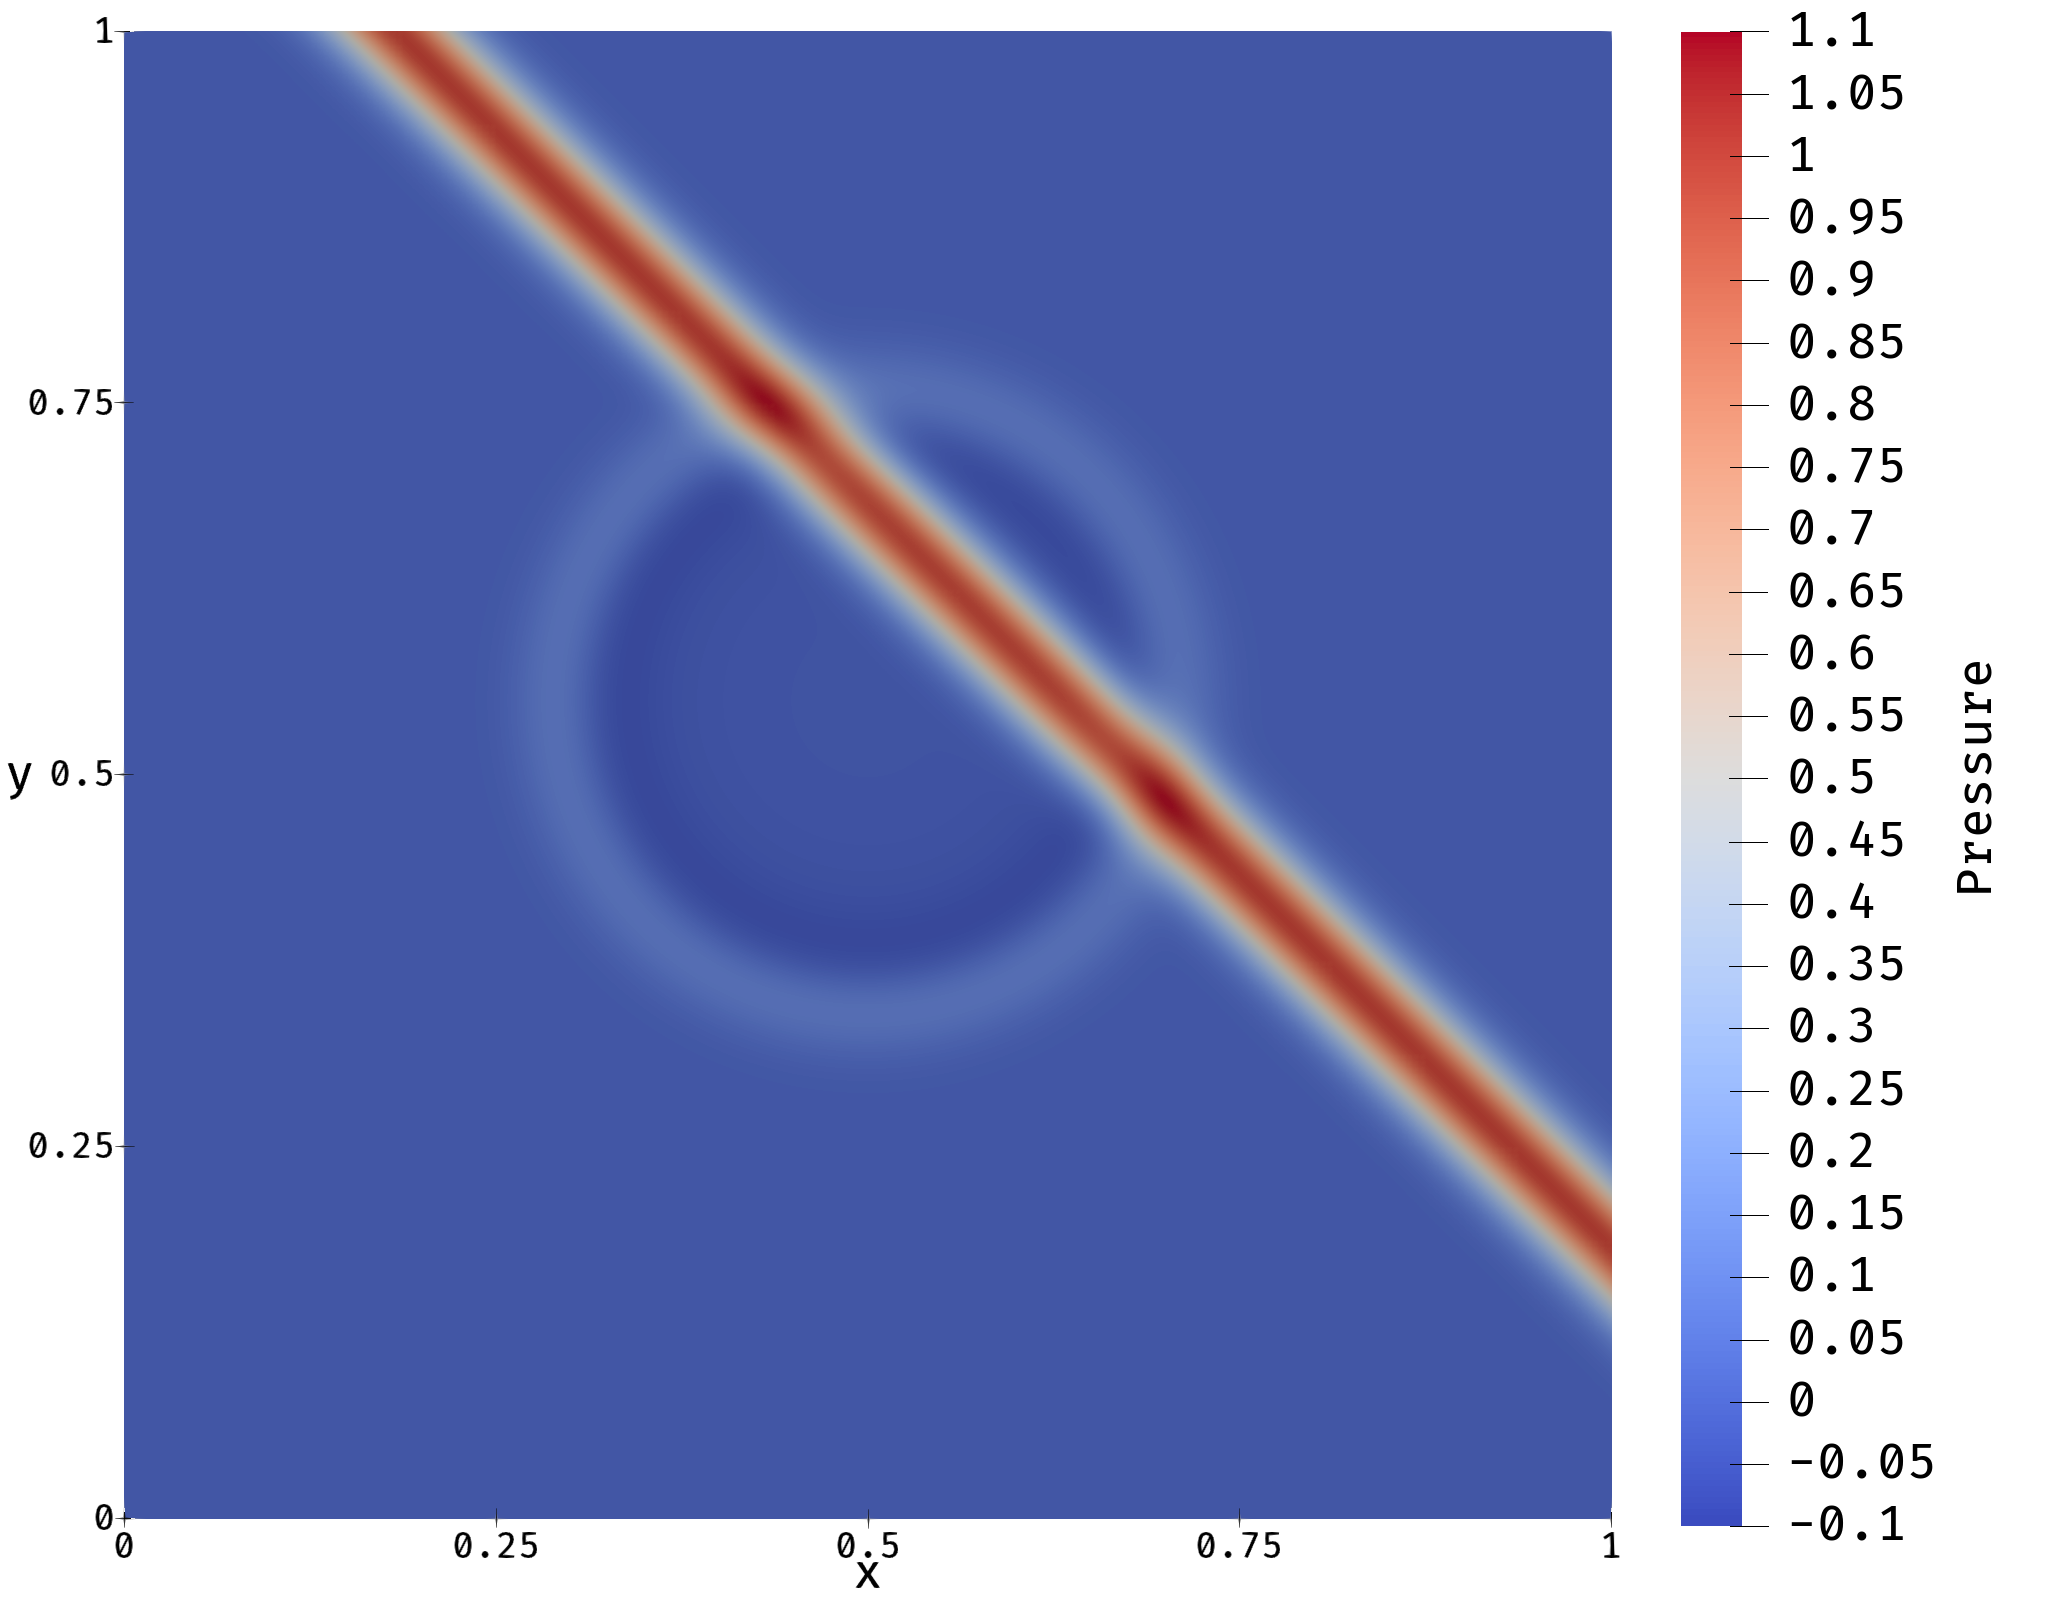
\includegraphics[width=0.48\textwidth]{Chapter_results/media/cloud_t0_2}\label{fig:cloud_p_t0_2}}
    \caption{Complex case: A wave goes through a cloud of high pressure. \(N_{initial} = 4\), \(K_{initial} = 256\), \(S = 3\), \(P = 16\) (a) Initial conditions (b) After the wave and cloud collide}\label{fig:cloud_p}
\end{figure}

\begin{figure}[H]
    \centering
    \subfloat[\( t = 0 s\)]
    {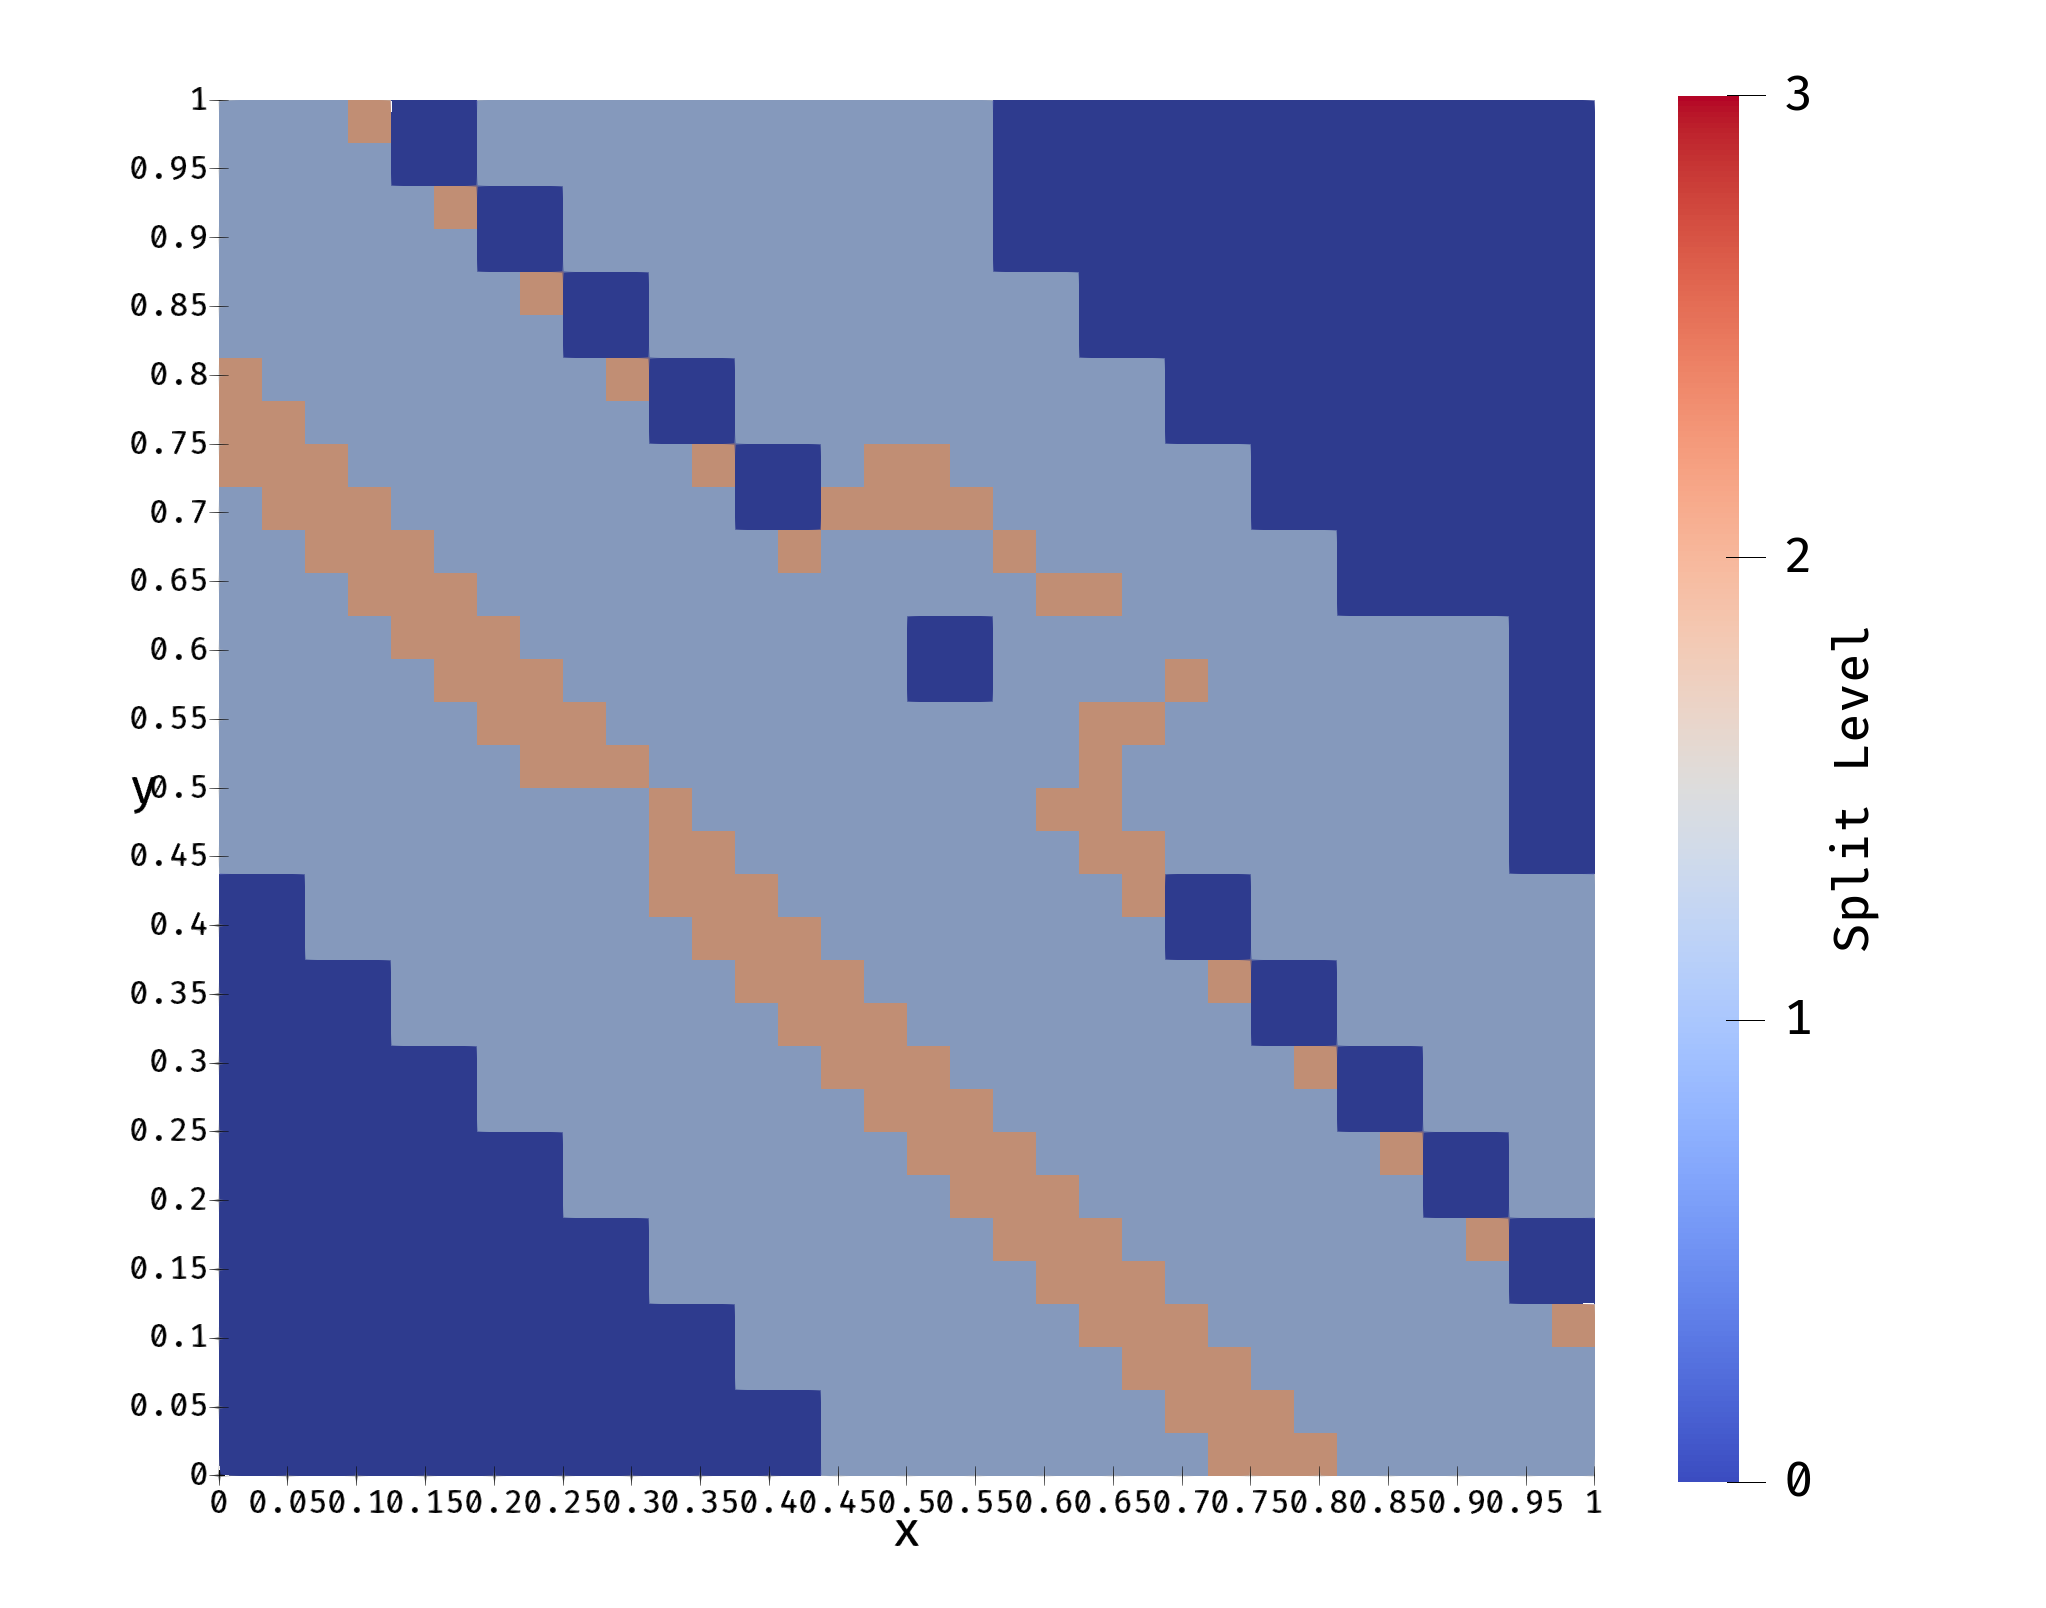
\includegraphics[width=0.48\textwidth]{Chapter_results/media/cloud_split_level_t0}\label{fig:cloud_s_t0}}
    \hfill
    \subfloat[\( t = 0.2 s\)]
    {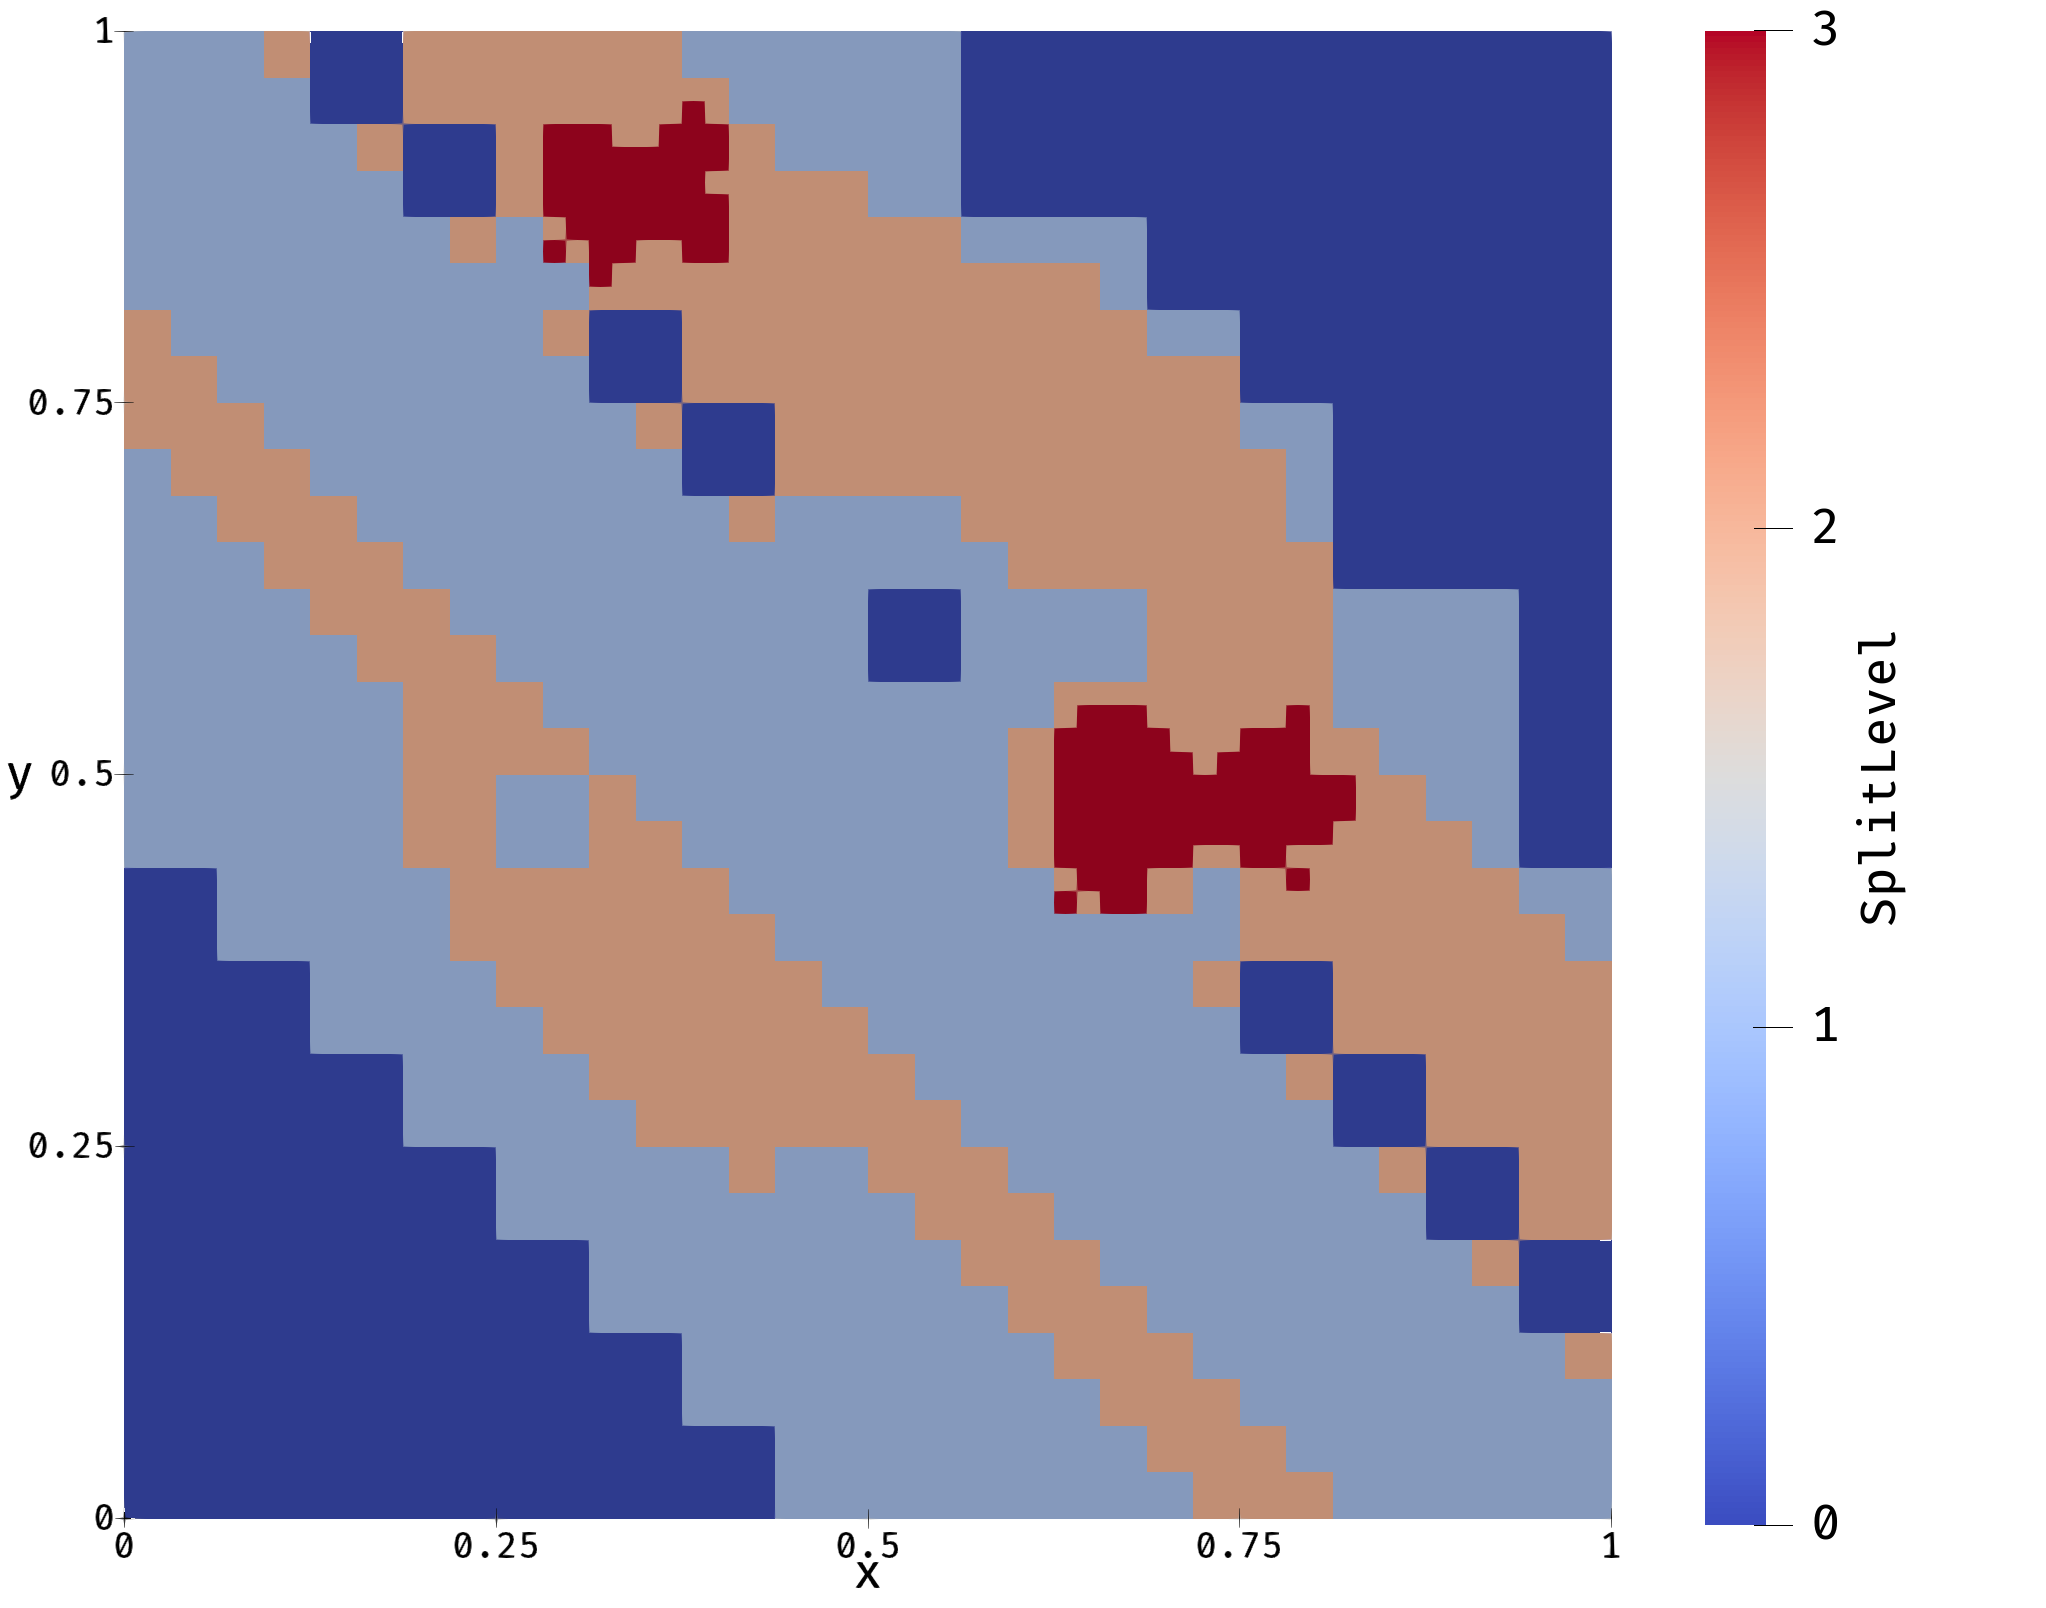
\includegraphics[width=0.48\textwidth]{Chapter_results/media/cloud_split_level_t0_2}\label{fig:cloud_s_t0_2}}
    \caption{Complex case h-refinement: The elements split more where the cloud meets the wave.
        \(N_{initial} = 4\), \(K_{initial} = 256\), \(S = 3\), \(P = 16\) (a) Start of time 
        advancing (b) After the wave and cloud collide}\label{fig:cloud_s}
\end{figure}

\begin{figure}[H]
    \centering
    \subfloat[\( t = 0 s\)]
    {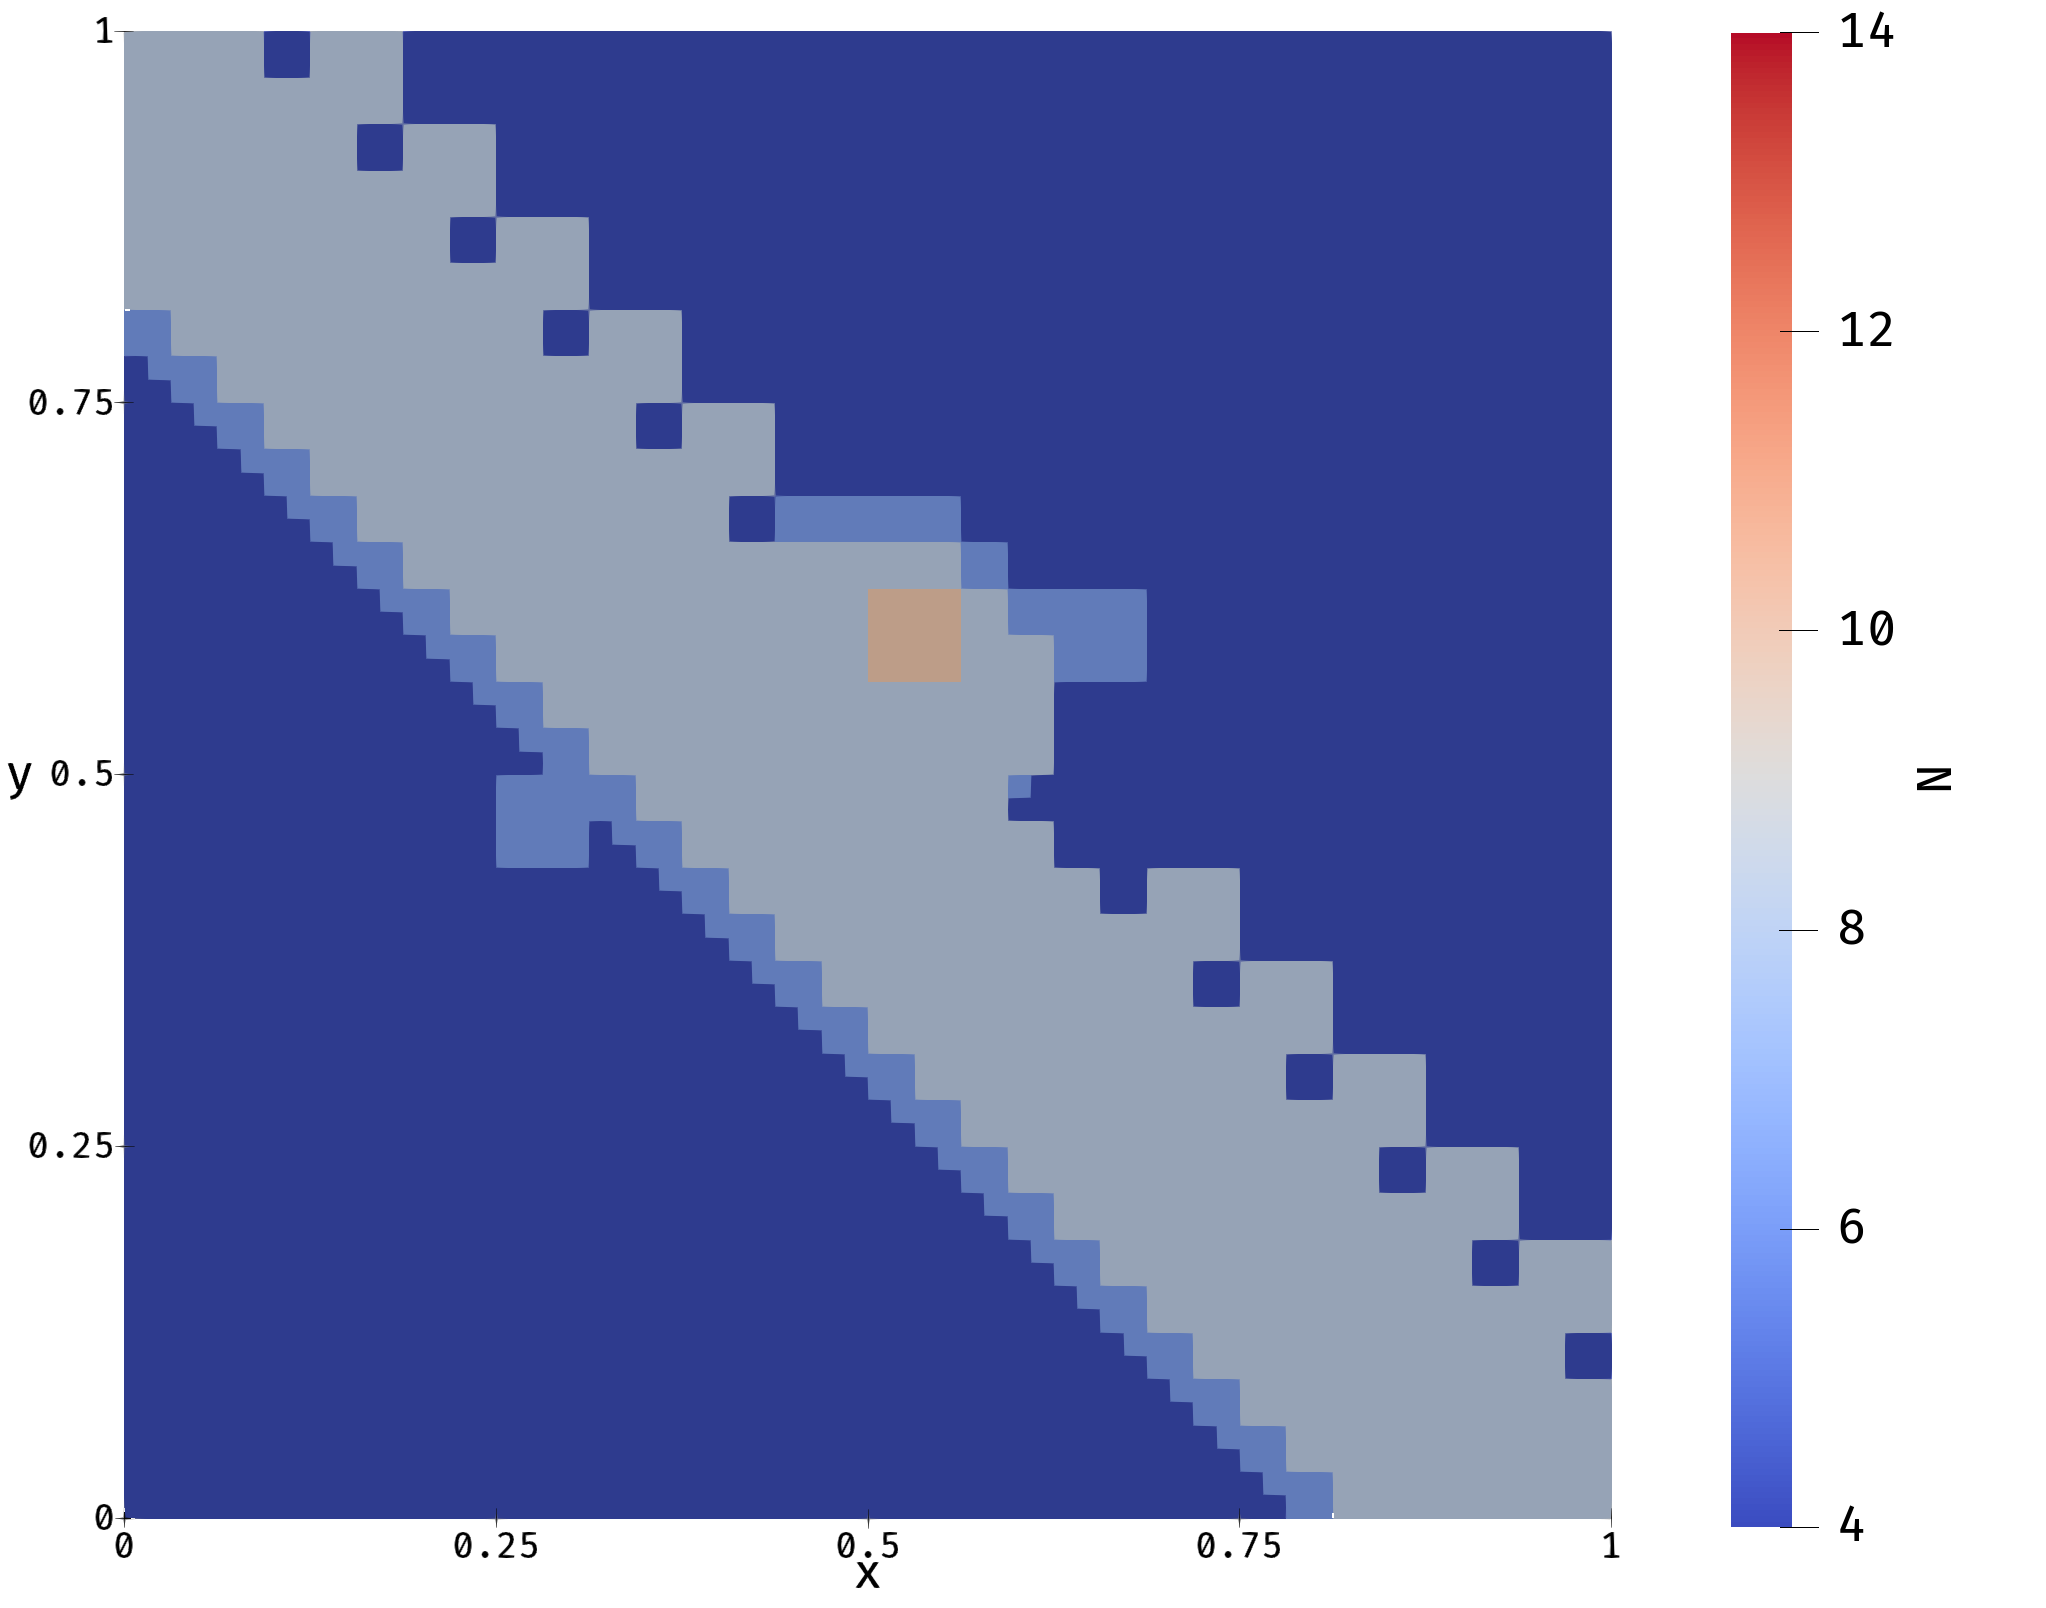
\includegraphics[width=0.48\textwidth]{Chapter_results/media/cloud_N_t0}\label{fig:cloud_N_t0}}
    \hfill
    \subfloat[\( t = 0.2 s\)]
    {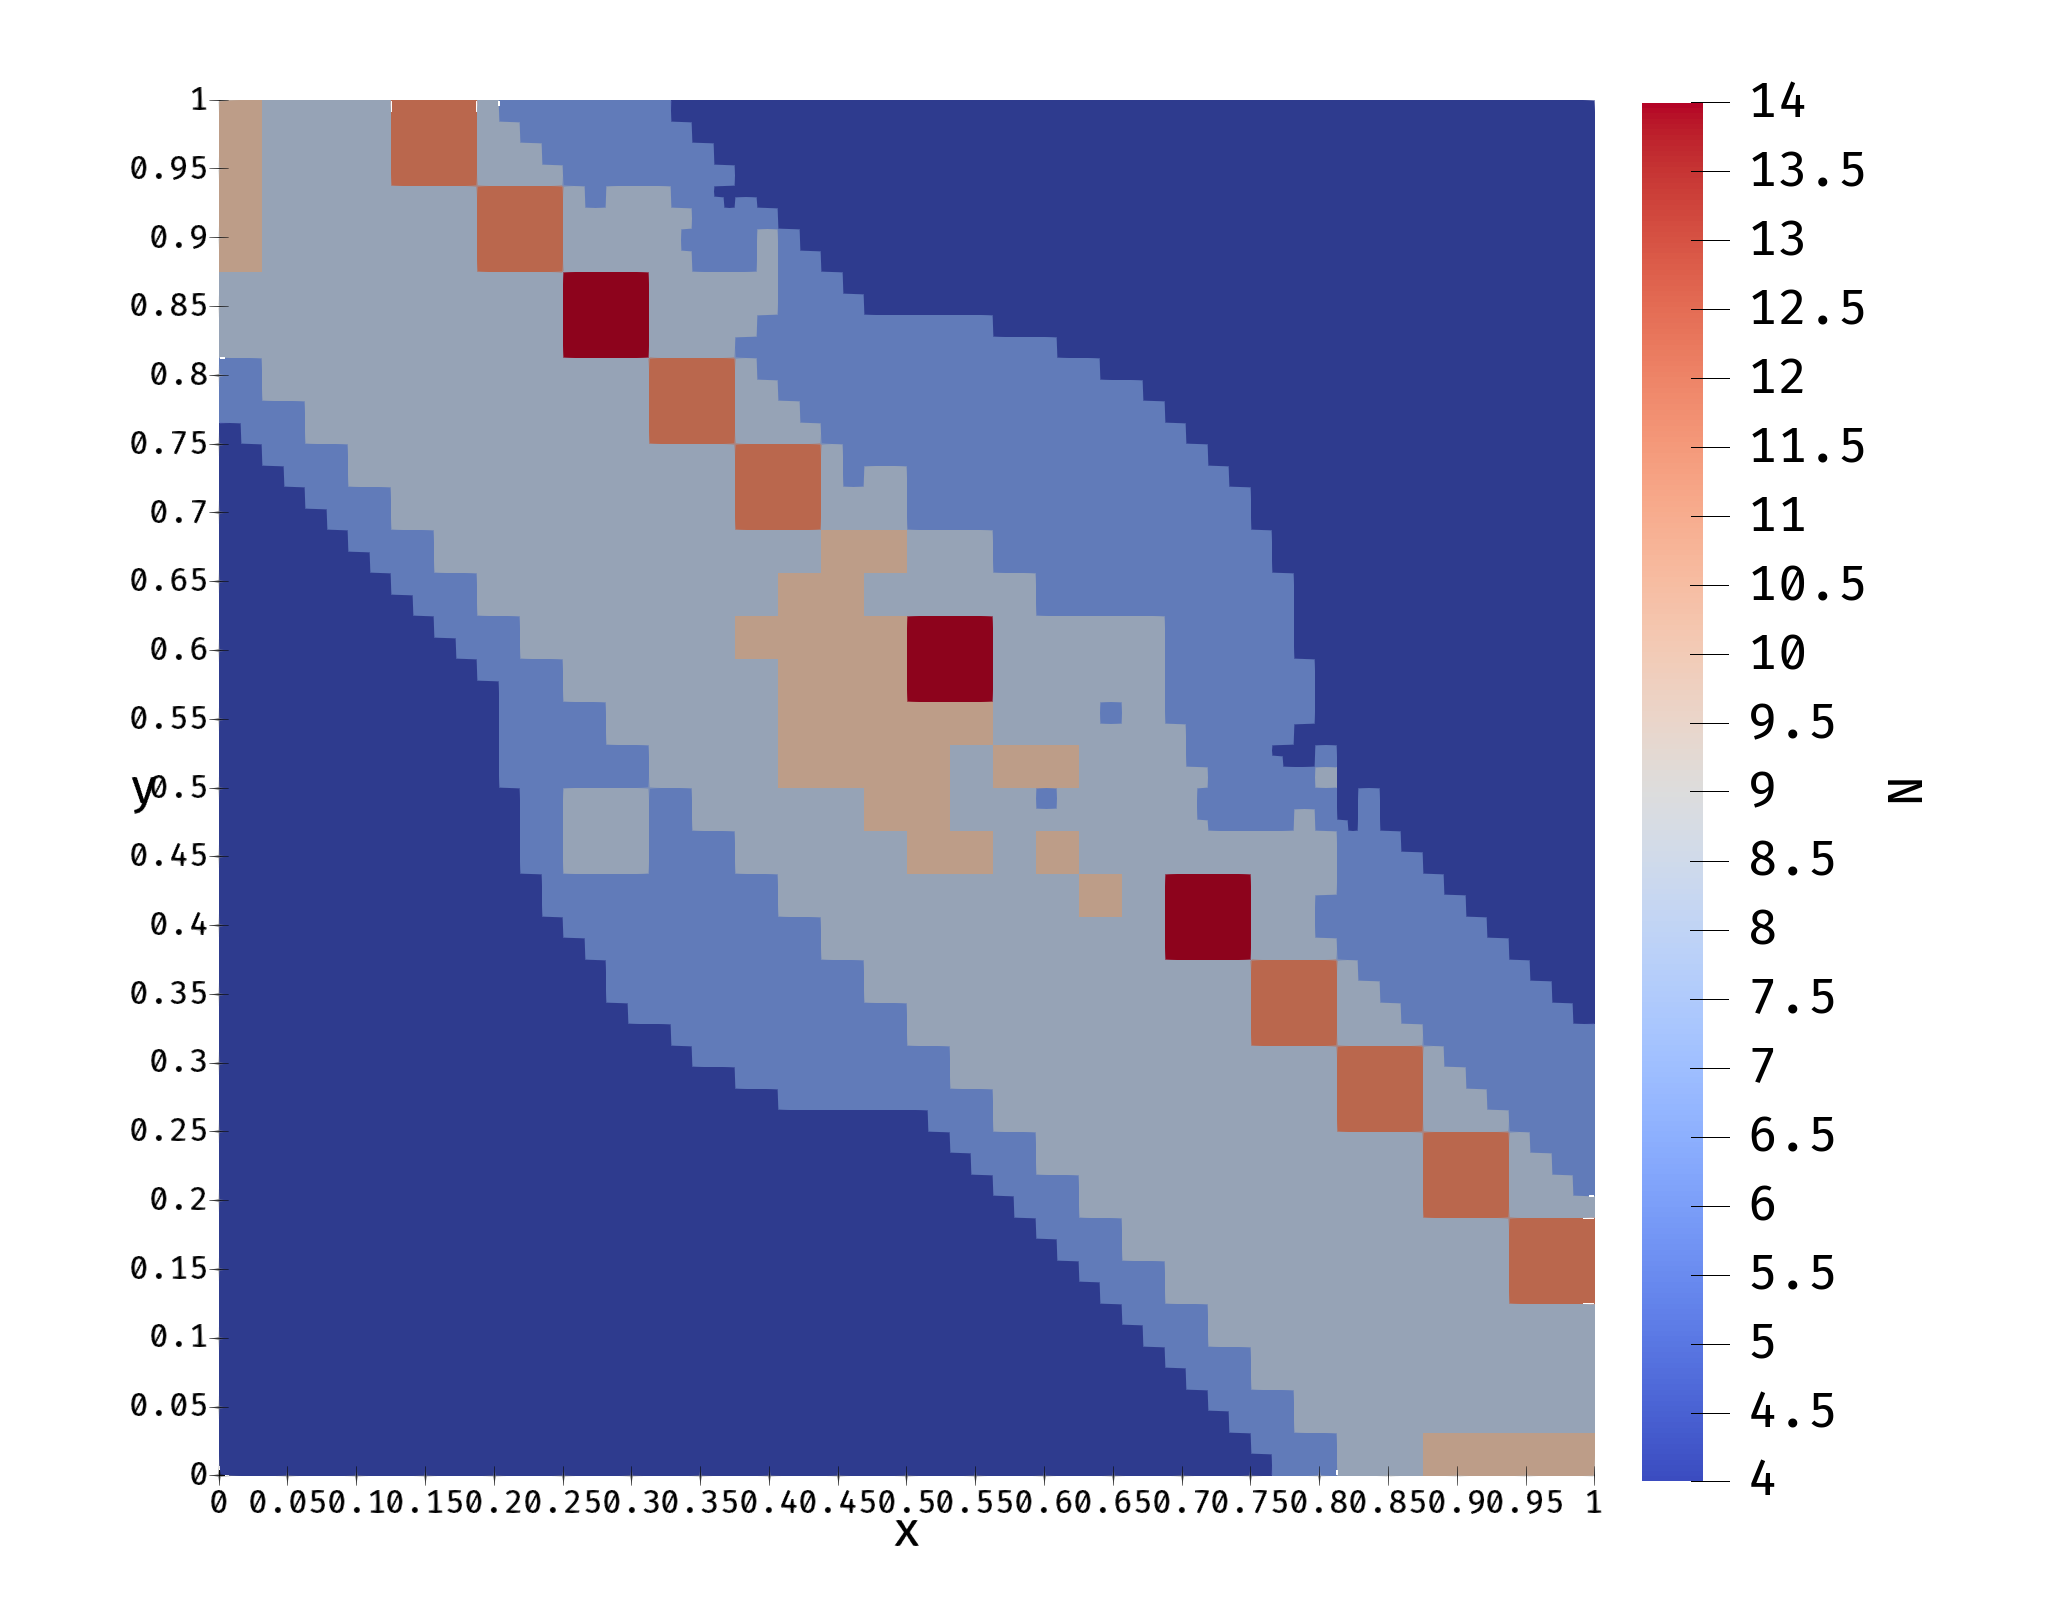
\includegraphics[width=0.48\textwidth]{Chapter_results/media/cloud_N_t0_2}\label{fig:cloud_N_t0_2}}
    \caption{Complex case p-refinement: The polynomial order increases more at the center of the
        cloud and where cloud meets the wave. \(N_{initial} = 4\), \(K_{initial} = 256\), \(S = 3\), 
        \(P = 16\) (a) Start of time advancing (b) After the wave and cloud 
        collide}\label{fig:cloud_N}
\end{figure}

\begin{figure}[H]
    \centering
    \subfloat[\( t = 0 s\)]
    {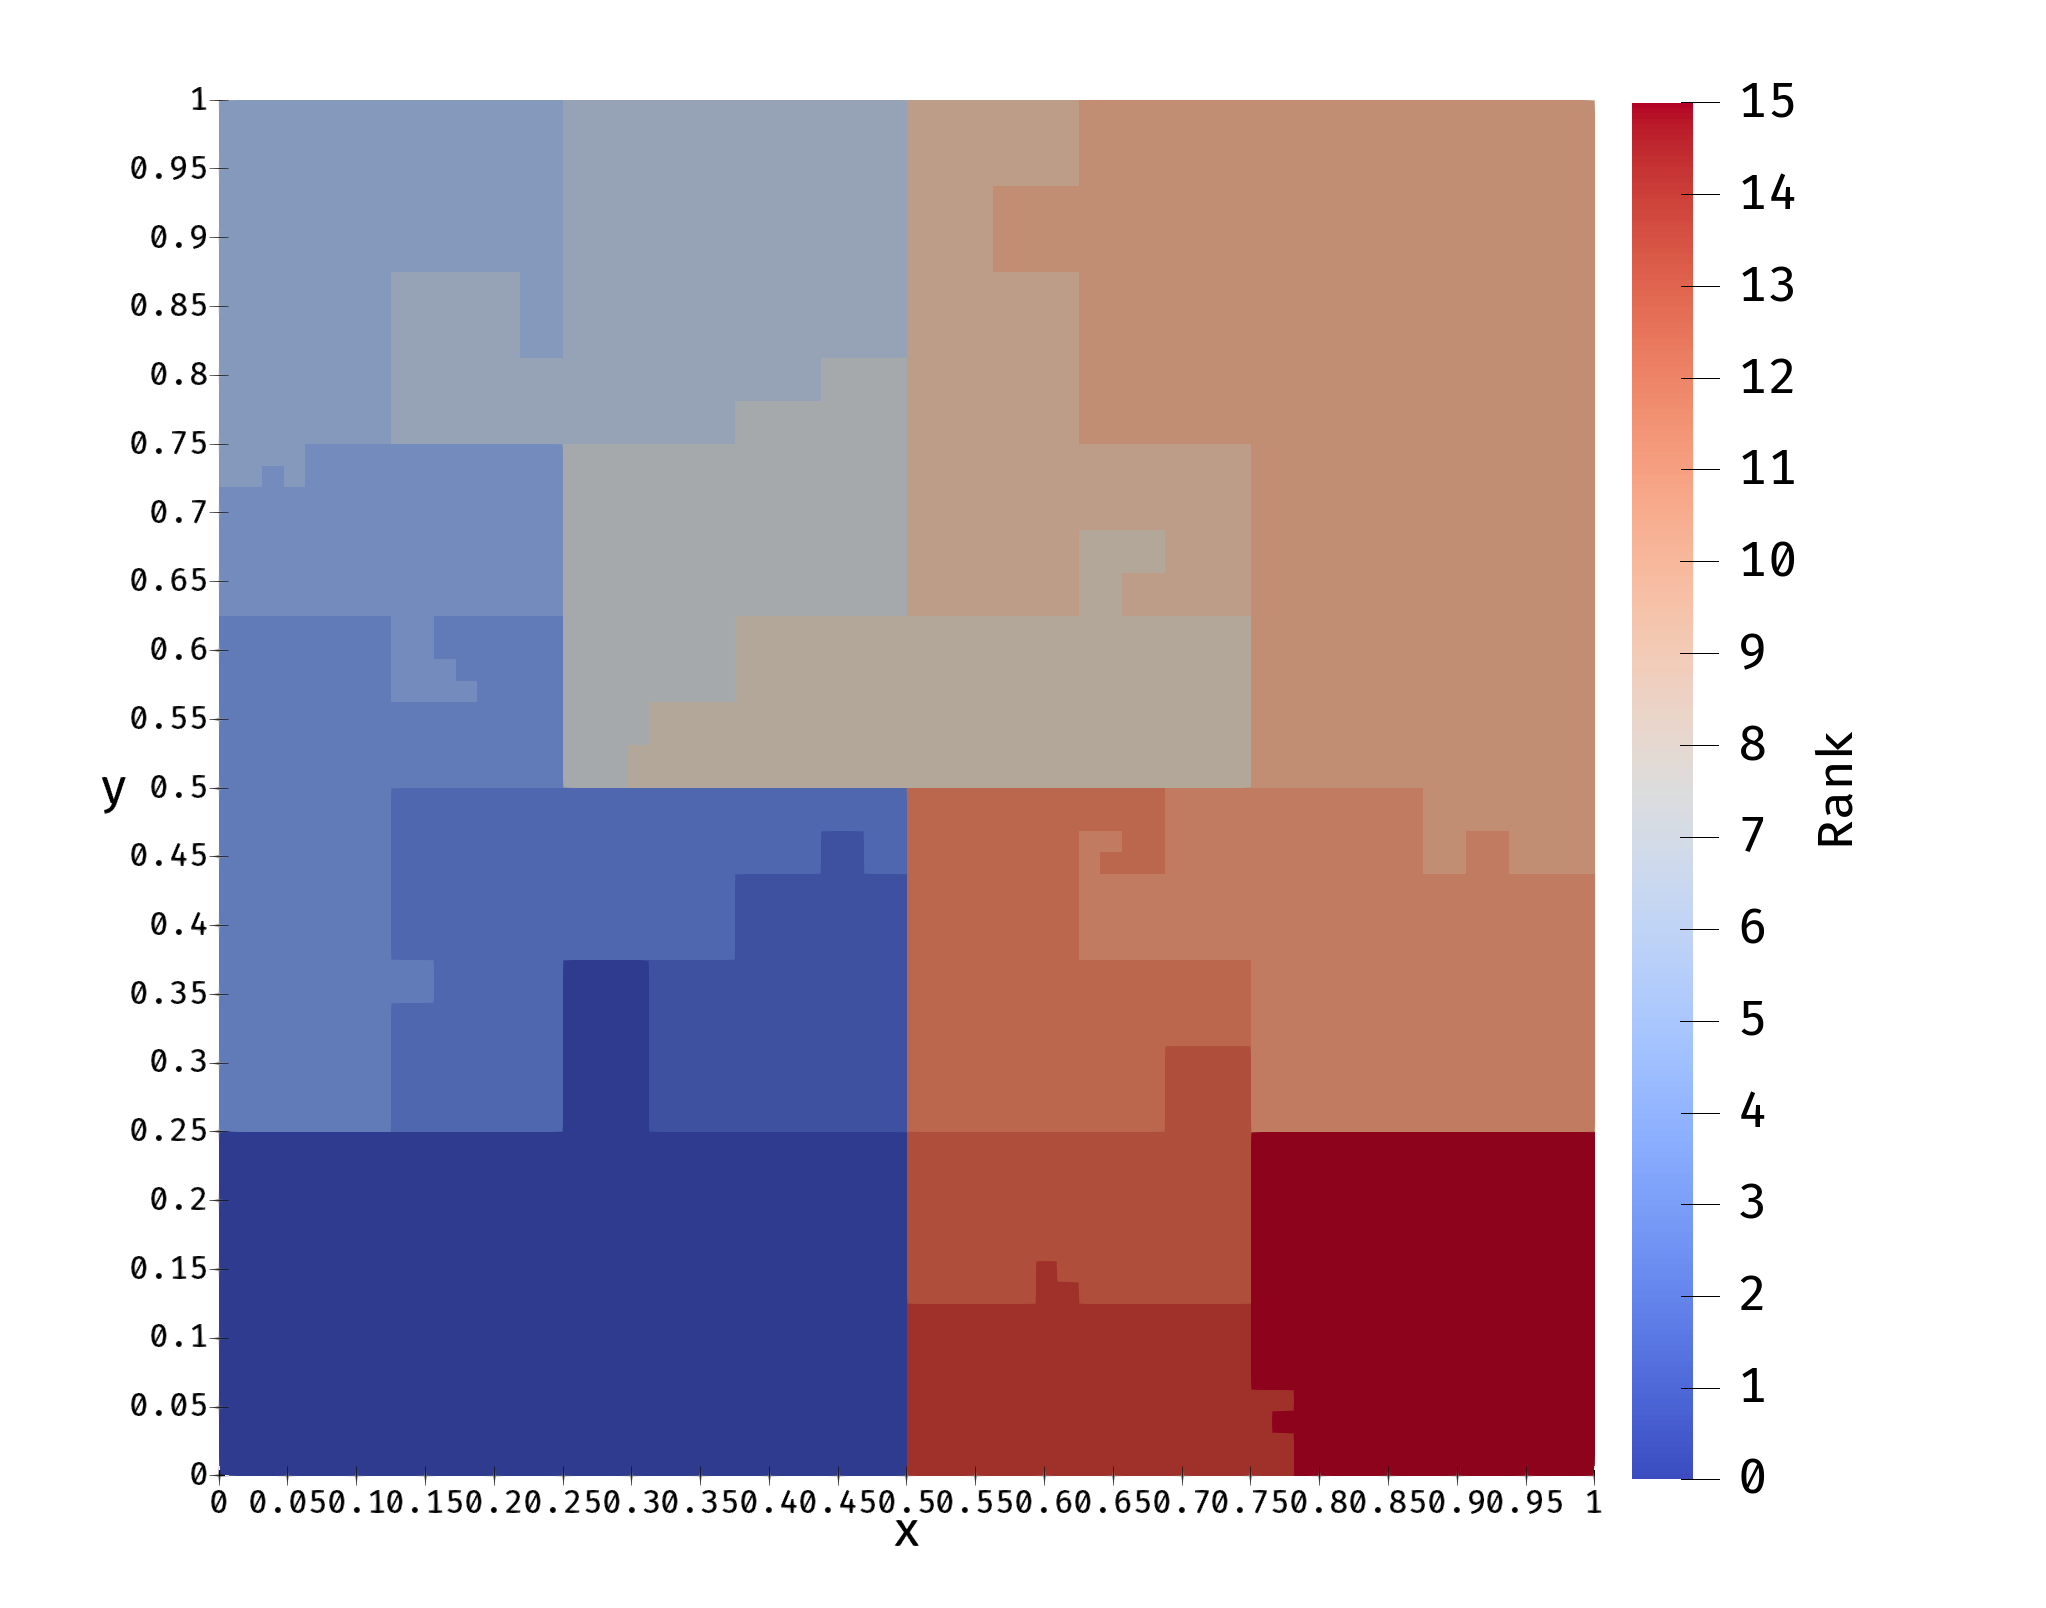
\includegraphics[width=0.48\textwidth]{Chapter_results/media/cloud_rank_t0}\label{fig:cloud_rank_t0}}
    \hfill
    \subfloat[\( t = 0.2 s\)]
    {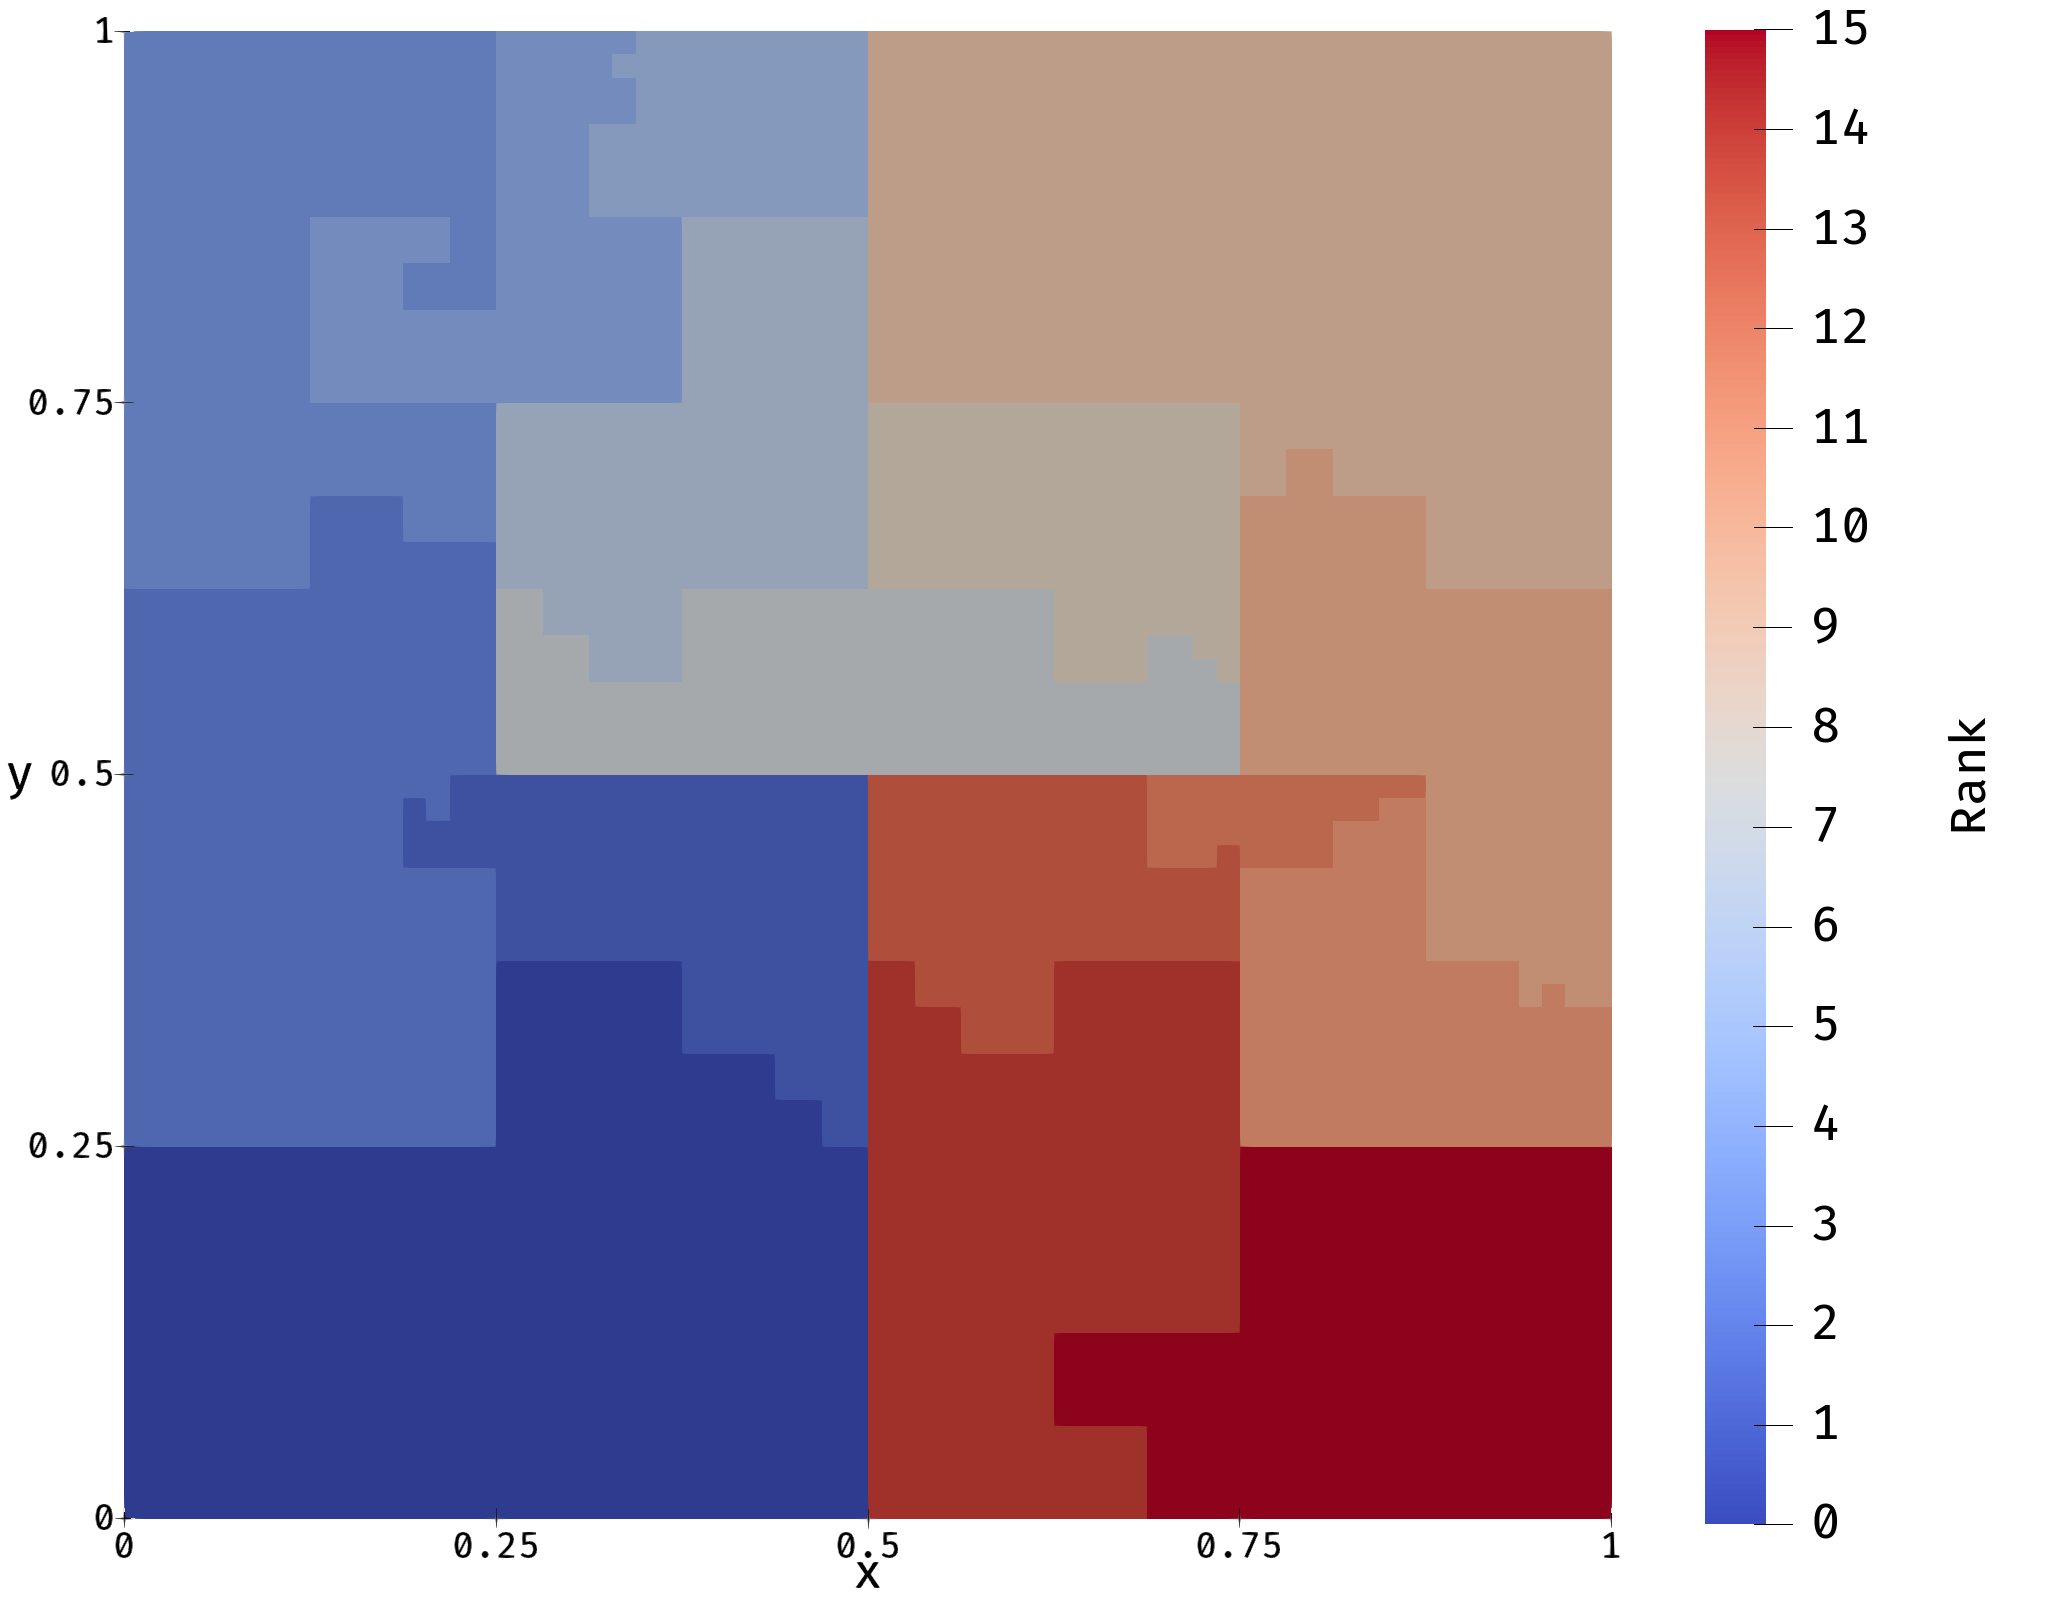
\includegraphics[width=0.48\textwidth]{Chapter_results/media/cloud_rank_t0_2}\label{fig:cloud_rank_t0_2}}
    \caption{Complex case rank: As the mesh is refined load imbalance can occur, and elements are
        sent from one \acrshort{acr:GPU} to another when load balancing. \(N_{initial} = 4\),
        \(K_{initial} = 256\), \(S = 3\), \(P = 16\) (a) Start of time advancing (b) After the wave 
        and cloud collide}\label{fig:cloud_rank}
\end{figure}

These figures show that the pre-condition steps do a good job of refining the mesh to capture the
initial conditions correctly in the \(t = 0 s\) figures (a). Afterwards,
Figures~\ref{fig:cloud_s_t0_2} and~\ref{fig:cloud_N_t0_2} show that the mesh is refined along the
movement of the linear wave and the expansion of the circular cloud, and is especially refined at
their intersection. This indicates that the error estimation correctly identifies the more difficult
areas of the solution. As more elements are created at the intersection of both waves, load
imbalance occurs, and by the end of the computation there are \(K = 5088\) elements. From
Figures~\ref{fig:cloud_s_t0_2} and~\ref{fig:cloud_rank_t0}, we can observe that there are more
h-refining elements around \acrshortpl{acr:GPU} \(6\) and \(8\), which are load balanced by \(t =
0.2 s\) in Figure~\ref{fig:cloud_rank_t0_2}. The elements are moved around by dynamic load
balancing, while keeping good locality and limiting the surface area between \acrshortpl{acr:GPU}.

\section{Complex Meshes}\label{section:results:complex_meshes}

We now introduce a case on a complex geometry to show that the program works with more complex
unstructured meshes that are not axis-aligned. Figure~\ref{fig:complex_mesh} shows the initial mesh
used for this case. Figure~\ref{fig:complex_mesh_pre_condition} shows the adapted mesh and
Figure~\ref{fig:complex_mesh_solution_p} depicts a wave moving across a NACA 0012 airfoil inside a
circular domain of radius \(20\). The mesh initially has \(K = 2128\) elements, is allowed to
h-refine up to \(S = 3\), and by the end of the computation there are \(K = 55680\) elements. The
polynomial order of the elements is initially \(N = 4\) and is allowed to p-refine up to \(N = 16\).
The mesh is refined every \(1000\) timesteps and load balanced with a imbalance threshold of \(L =
1.1\). At the beginning of the computation, three pre-condition steps are performed, which is why
the mesh is already refined at \(t = 0 s\) in Figure~\ref{fig:complex_mesh_pre_condition_far}. The
solution is computed in parallel on \(P = 4\) \acrshortpl{acr:GPU}.

The mesh is unstructured, and the original mesh file is numbered in a way that places elements with
neighbouring indices very far apart in the 2D domain. This is not ideal, as it scatters memory
accesses in a way that is detrimental to \acrshort{acr:GPU} performance, and increases dramatically
the number of inter-\acrshort{acr:GPU} boundaries. To improve the numbering, the mesh was renumbered
to a pseudo-Hilbert curve according to an algorithm presented in Appendix~\ref{chapter:renumbering}.
It is not a real Hilbert curve, as the Hilbert curve is only defined in 2D square domains with a
power of two number of axis-aligned elements in both dimensions. Nonetheless, this pseudo-Hilbert
curve resembles the Hilbert curve, and improves locality.

\begin{figure}[H]
    \centering
    \subfloat[Circular domain]
    {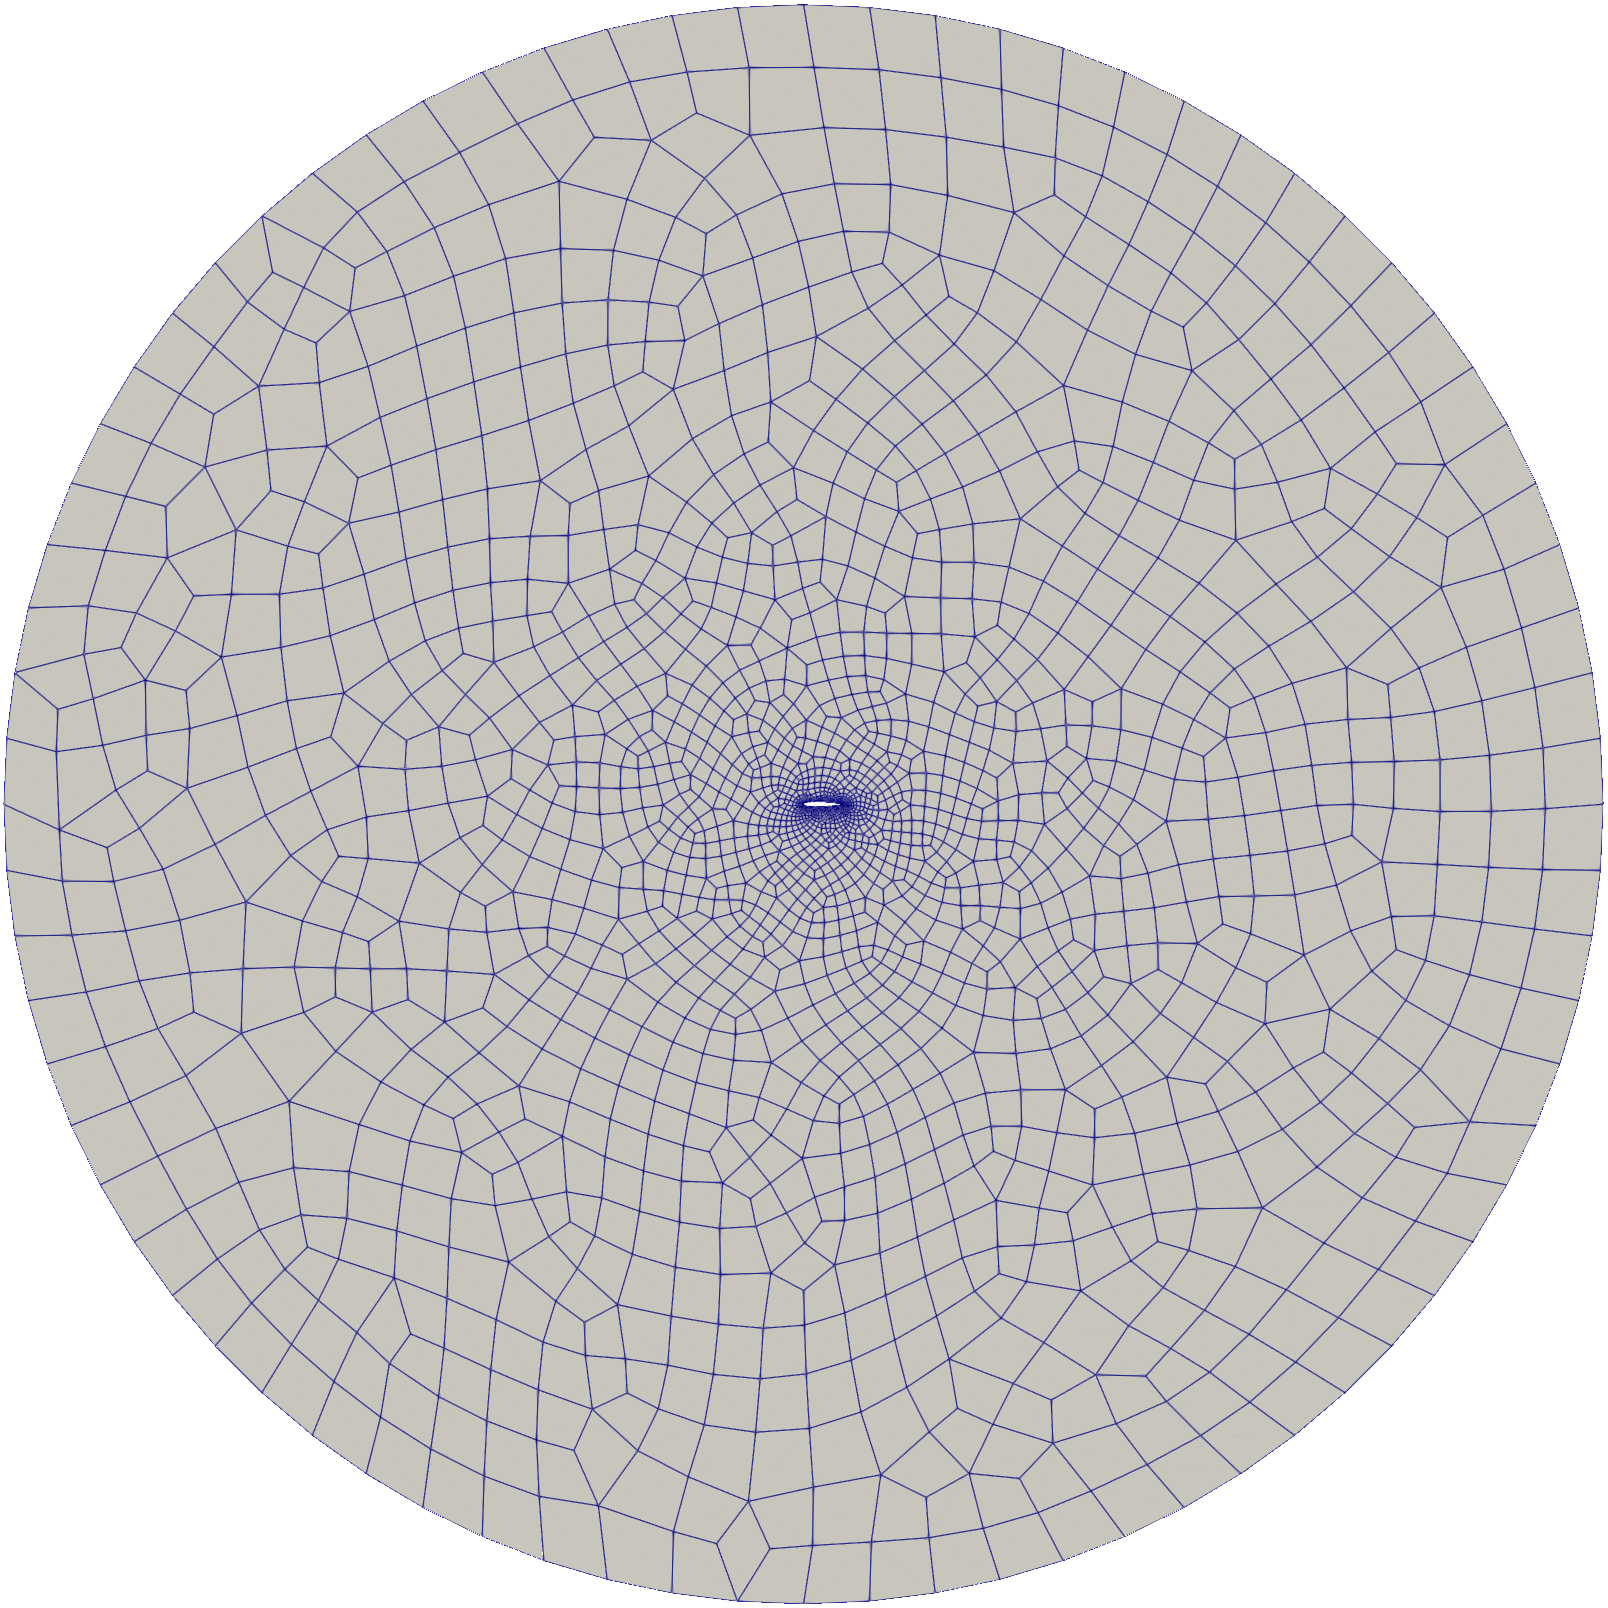
\includegraphics[width=0.48\textwidth]{Chapter_results/media/airfoil_mesh_far}\label{fig:complex_mesh_far}}
    \hfill
    \subfloat[Airfoil]
    {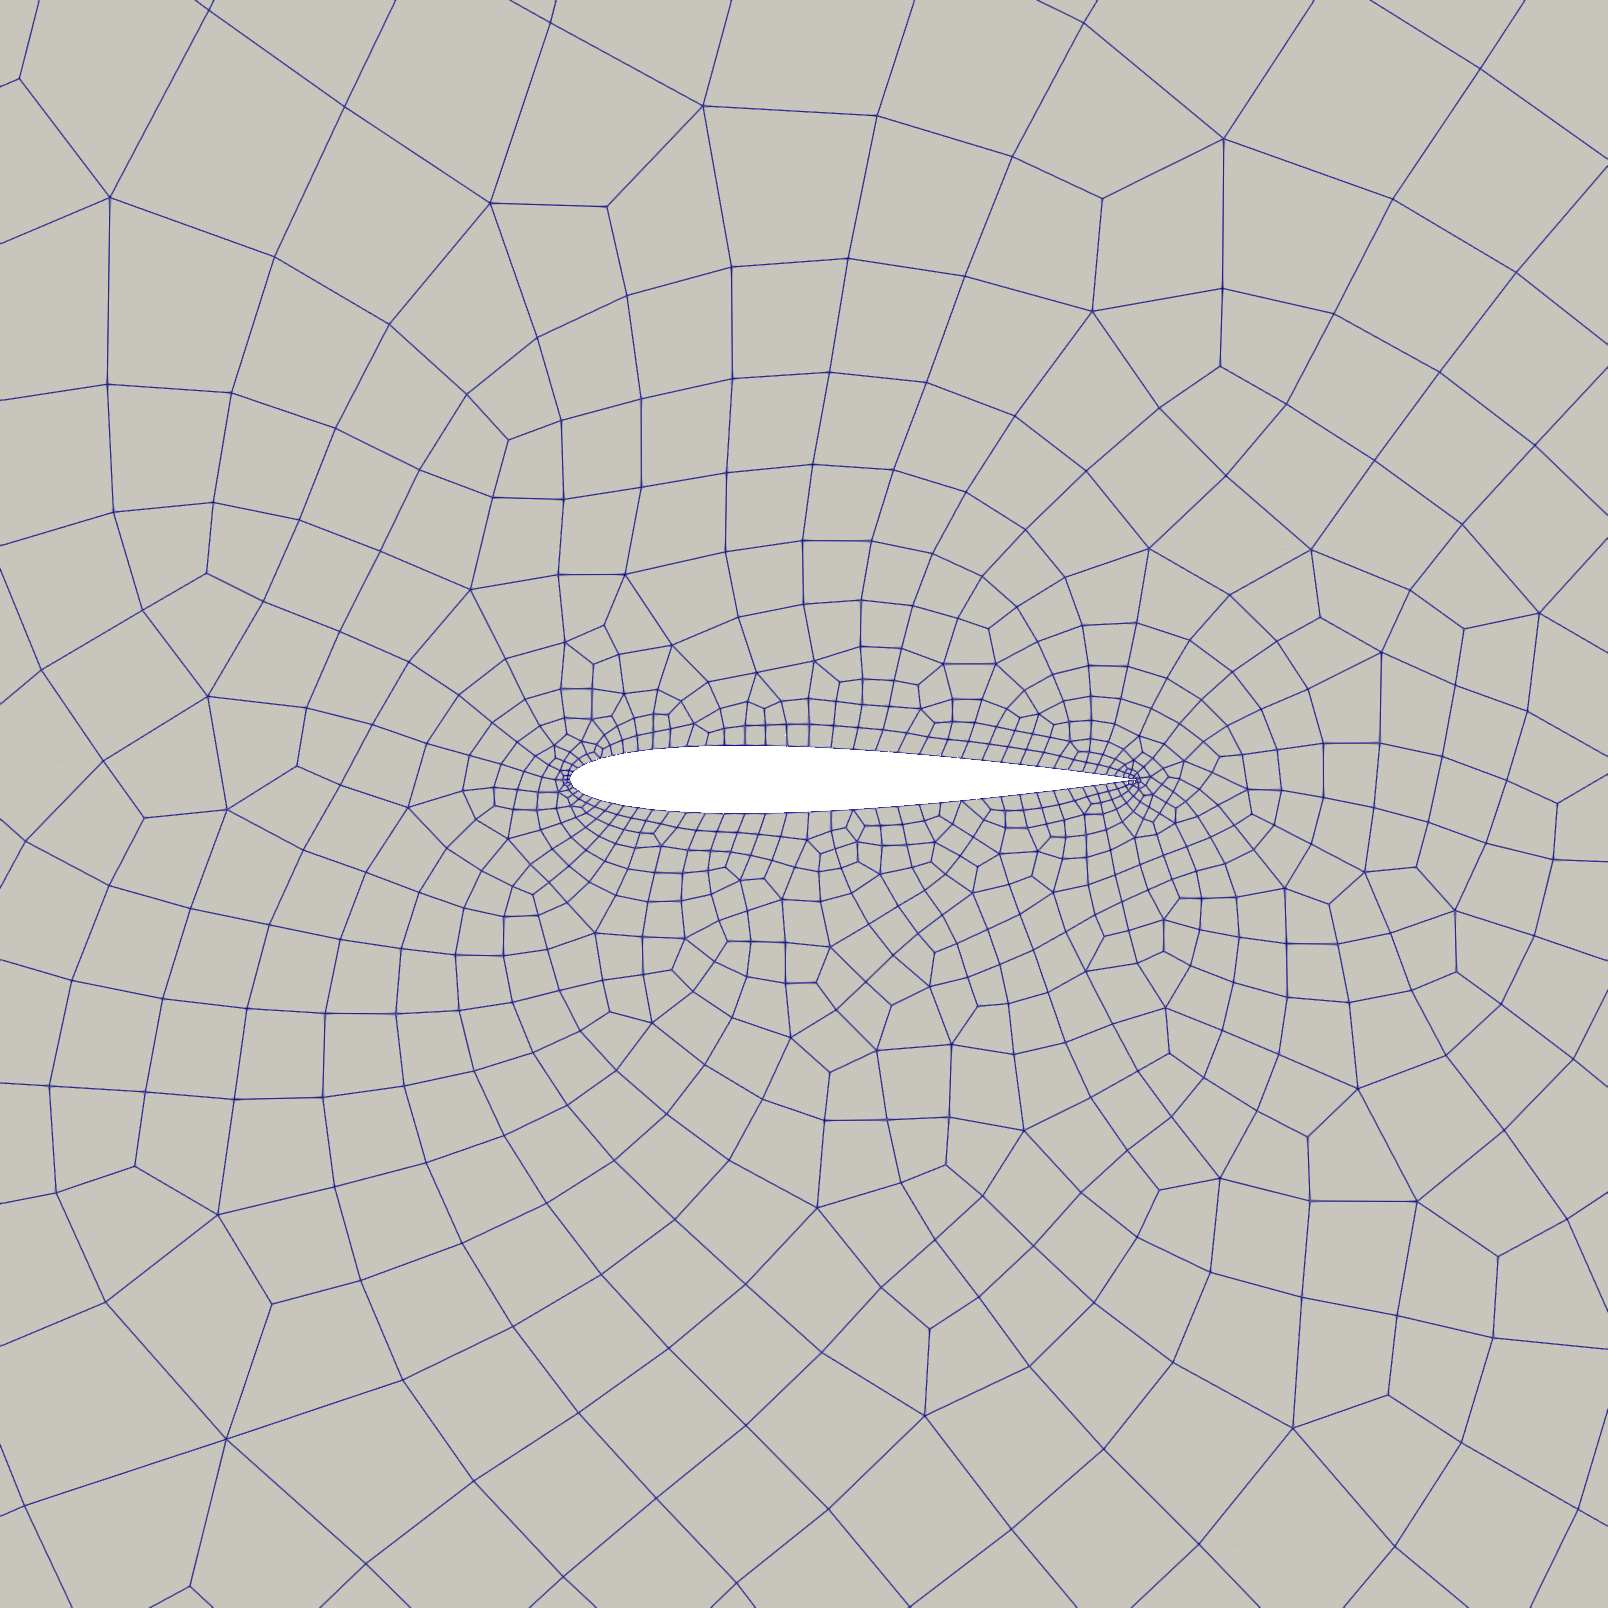
\includegraphics[width=0.48\textwidth]{Chapter_results/media/airfoil_mesh_near}\label{fig:complex_mesh_near}}
    \caption{Complex mesh example: An airfoil in an unstructured circular domain with its initial 
        mesh. \(N_{initial} = 4\), \(K_{initial} = 2128\), \(S = 3\), \(P = 4\) (a) Complete domain 
        (b) Up close}\label{fig:complex_mesh}
\end{figure}

\begin{figure}[H]
    \centering
    \subfloat[Circular domain]
    {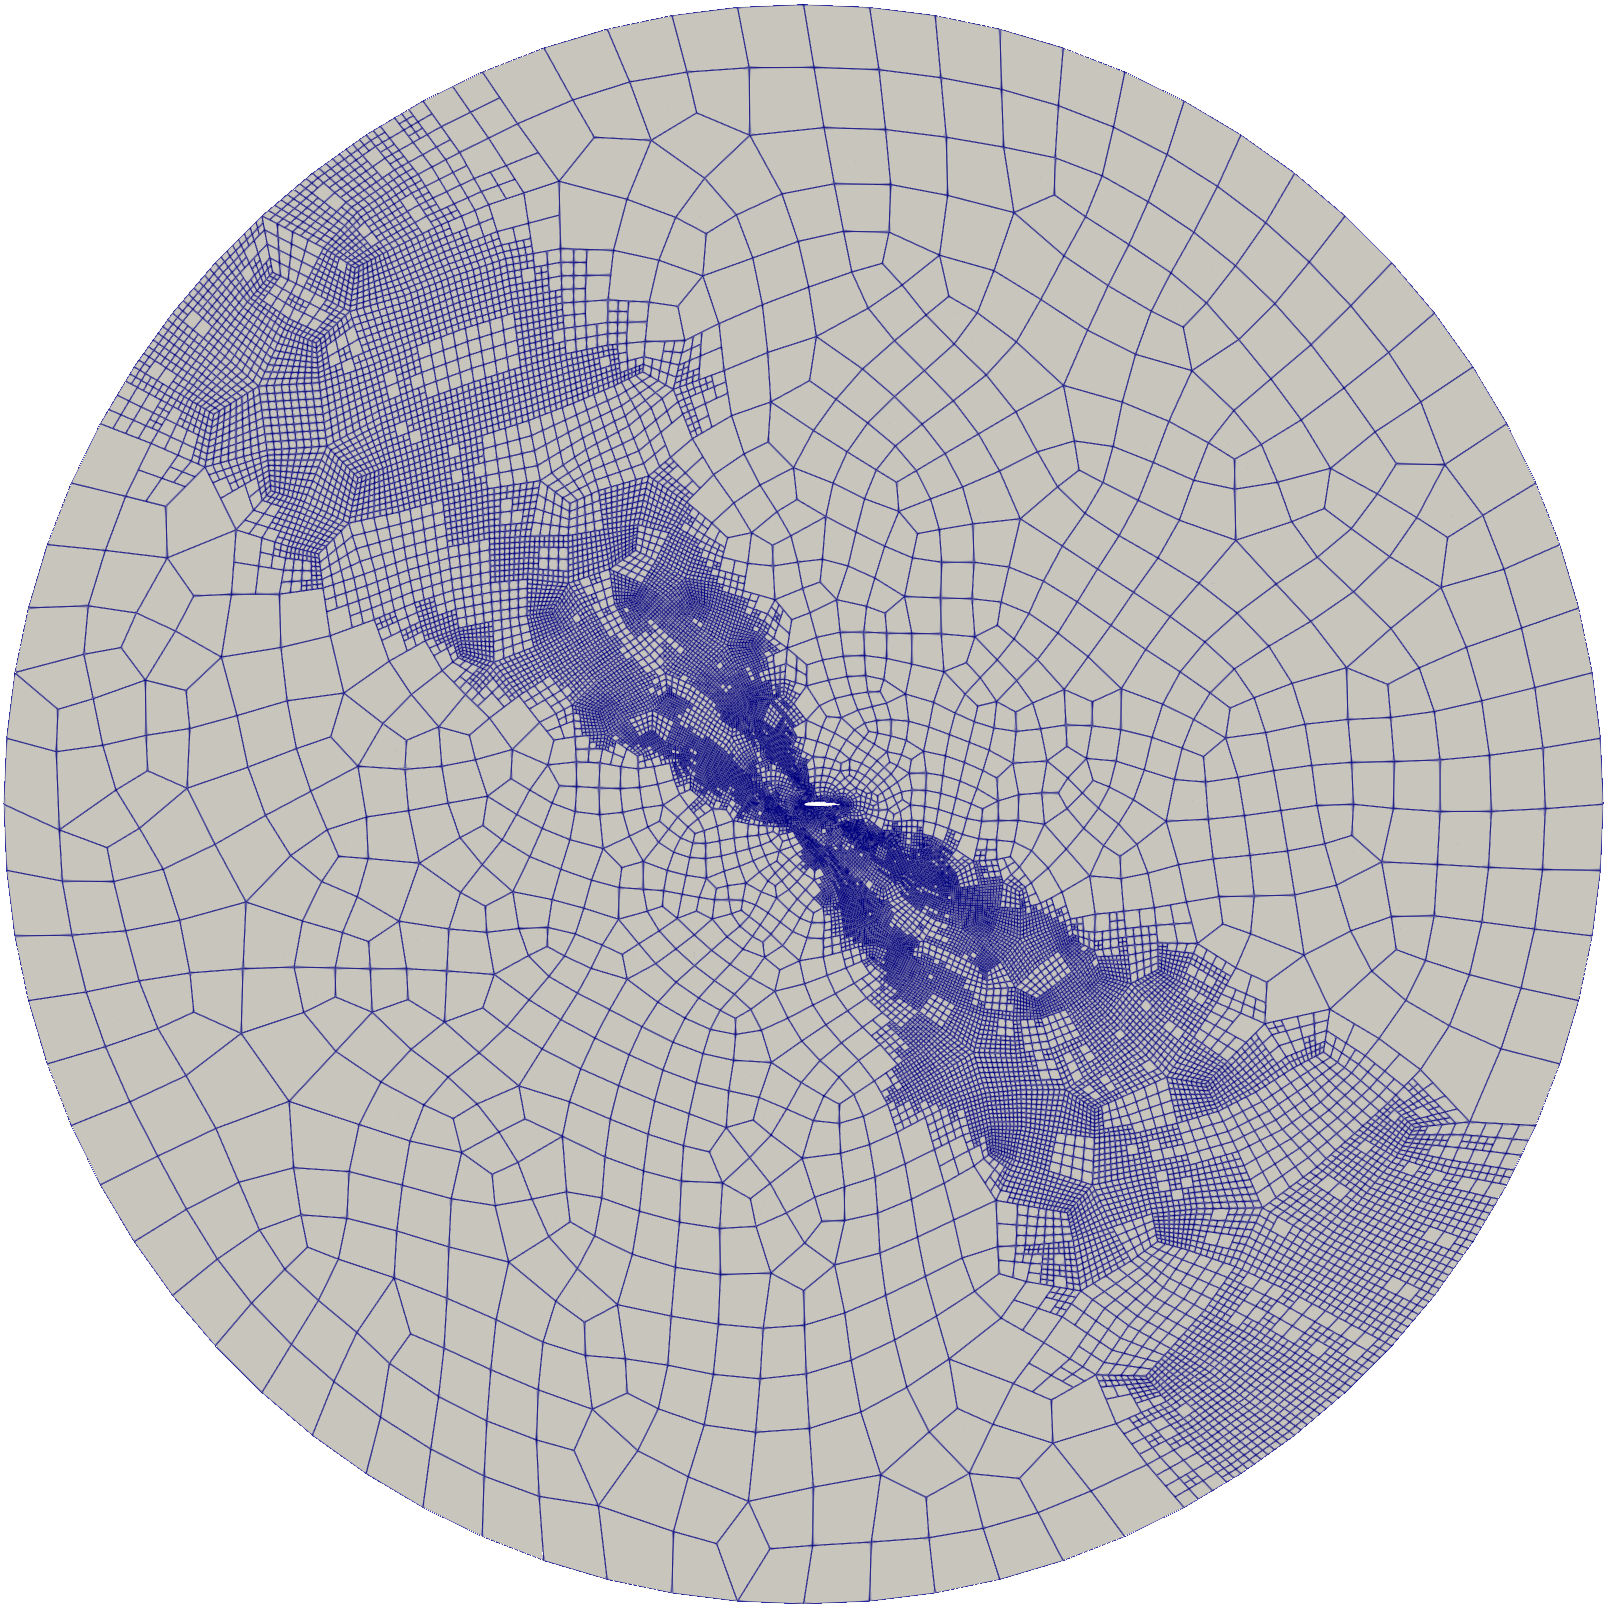
\includegraphics[width=0.48\textwidth]{Chapter_results/media/airfoil_mesh_pre_condition_far}\label{fig:complex_mesh_pre_condition_far}}
    \hfill
    \subfloat[Airfoil]
    {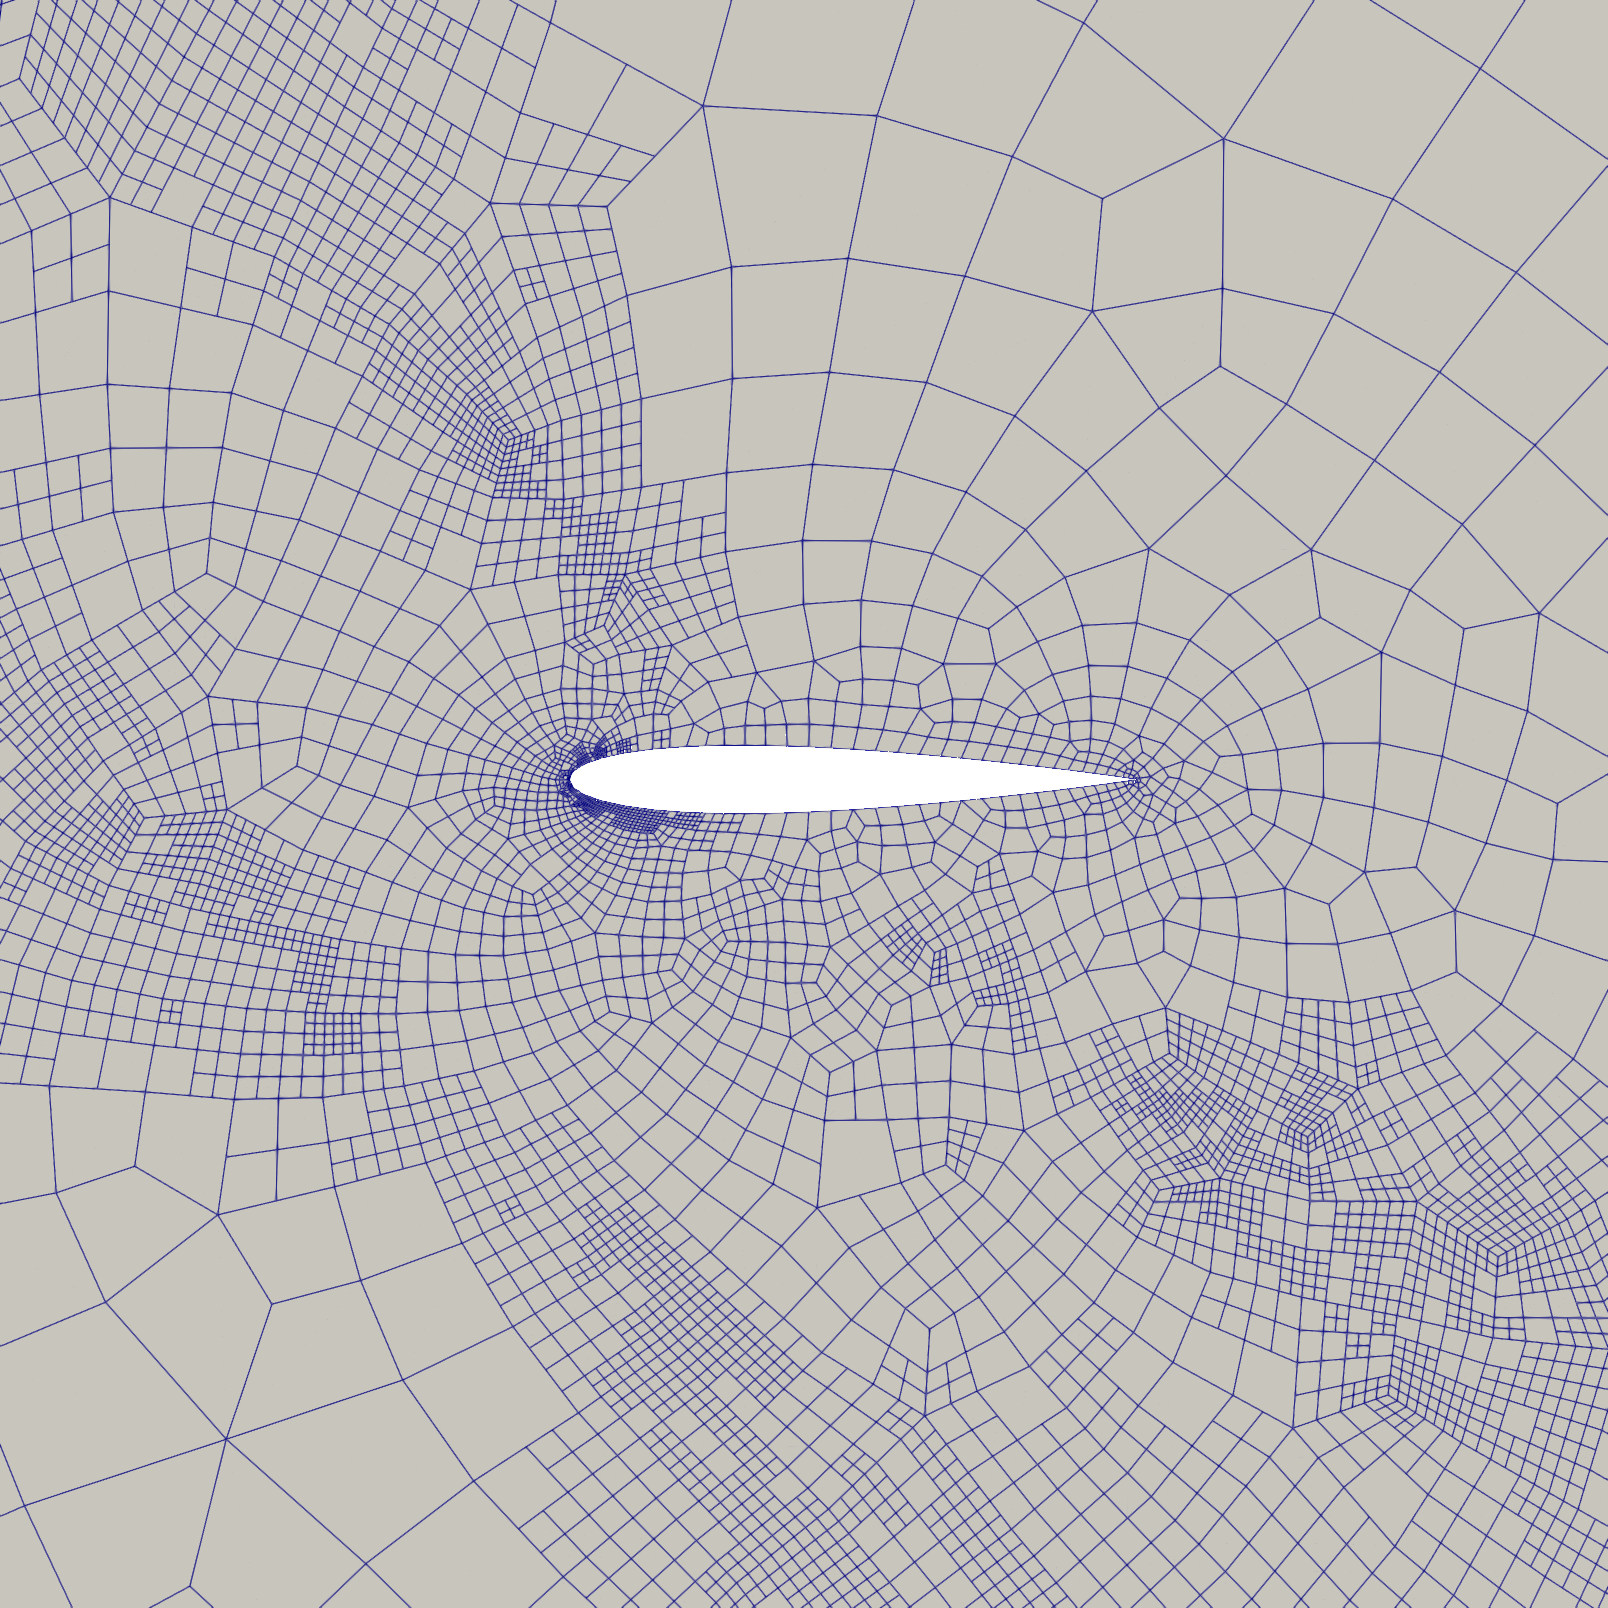
\includegraphics[width=0.48\textwidth]{Chapter_results/media/airfoil_mesh_pre_condition_near}\label{fig:complex_mesh_pre_condition_near}}
    \caption{Complex mesh after pre-condition: Elements have been added to better apply initial 
        conditions. \(N_{initial} = 4\), \(K = 24072\), \(S = 3\), \(P = 4\) (a) Complete domain (b) 
        Up close}\label{fig:complex_mesh_pre_condition}
\end{figure}

Figure~\ref{fig:complex_mesh_solution} shows the problem after \(1.5\) seconds of solution time.
Figure~\ref{fig:complex_mesh_solution_p} shows the pressure distribution, the wave having passed
around the airfoil and created a reflected circular wave.
Figure~\ref{fig:complex_mesh_solution_sigma} shows the pressure error decay rate \(\sigma \), which
informs the decision between h-refinement and p-refinement. An orange value, above \(1\), indicates
p-refinement would be chosen, whereas a blue value, below \(1\), indicates h-refinement would be
chosen. Figure~\ref{fig:complex_mesh_split_level} shows the split level \(S\), denoting how many
times elements have h-refined. Figure~\ref{fig:complex_mesh_N} shows the polynomial order \(N\),
which increases when elements are p-refined.

\begin{figure}[H]
    \centering

    \subfloat[Pressure]
    {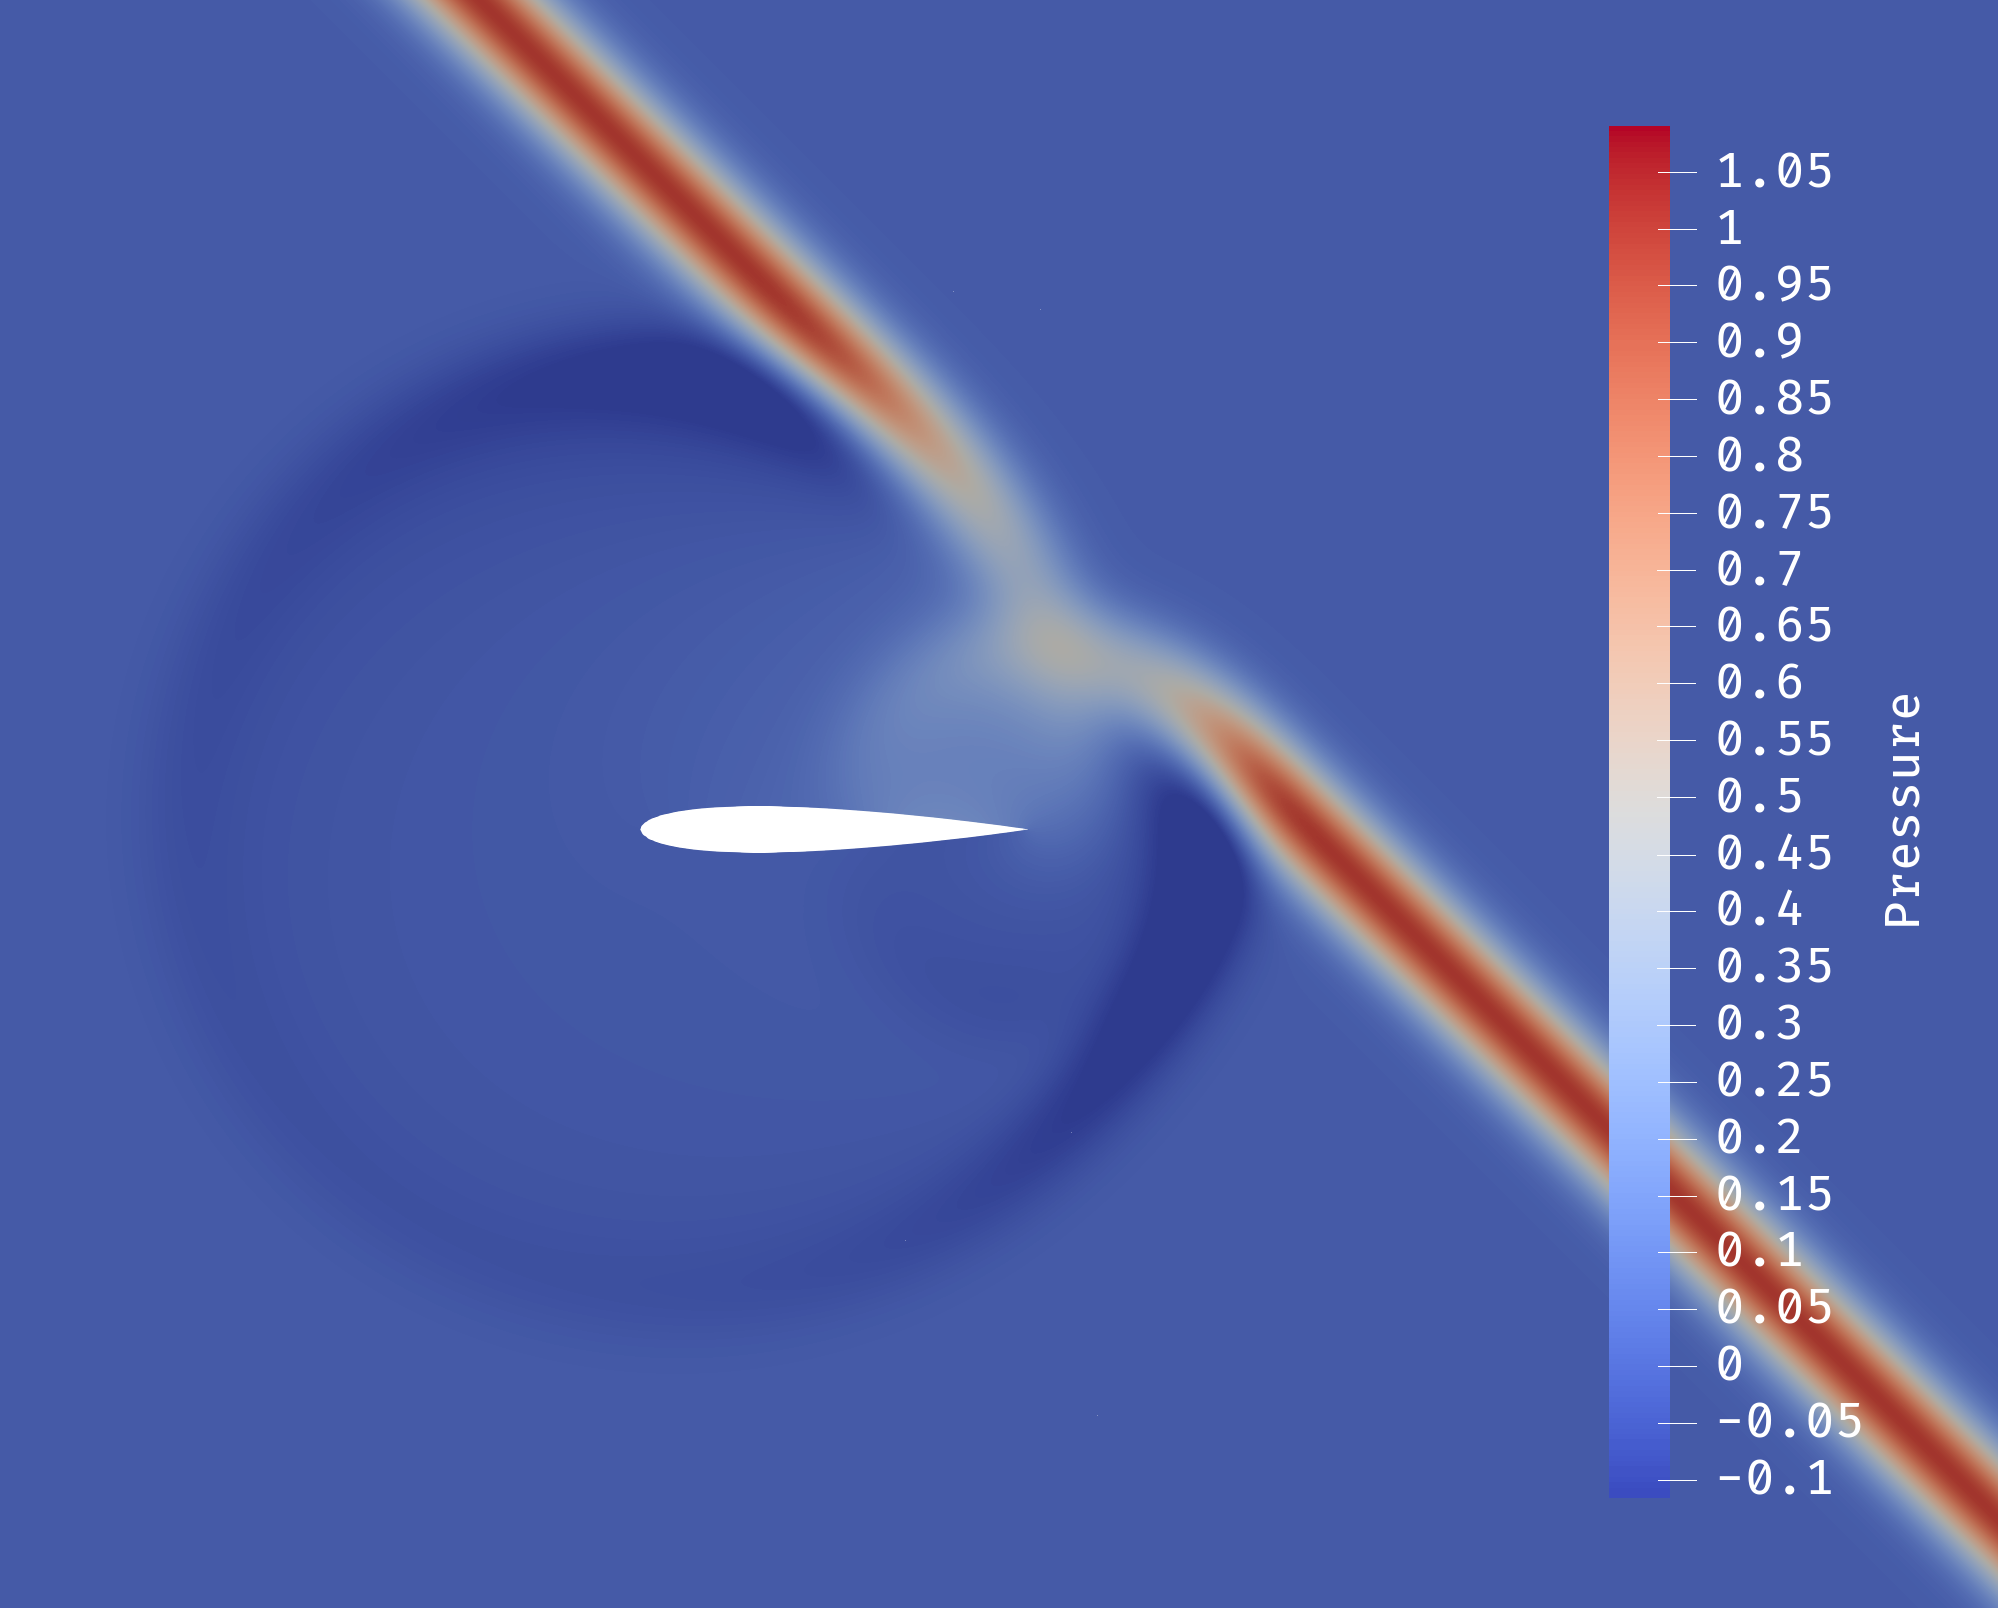
\includegraphics[width=0.48\textwidth]{Chapter_results/media/airfoil_pressure_near_t1_5}\label{fig:complex_mesh_solution_p}}
    \hfill
    \subfloat[Pressure \(\sigma \)]
    {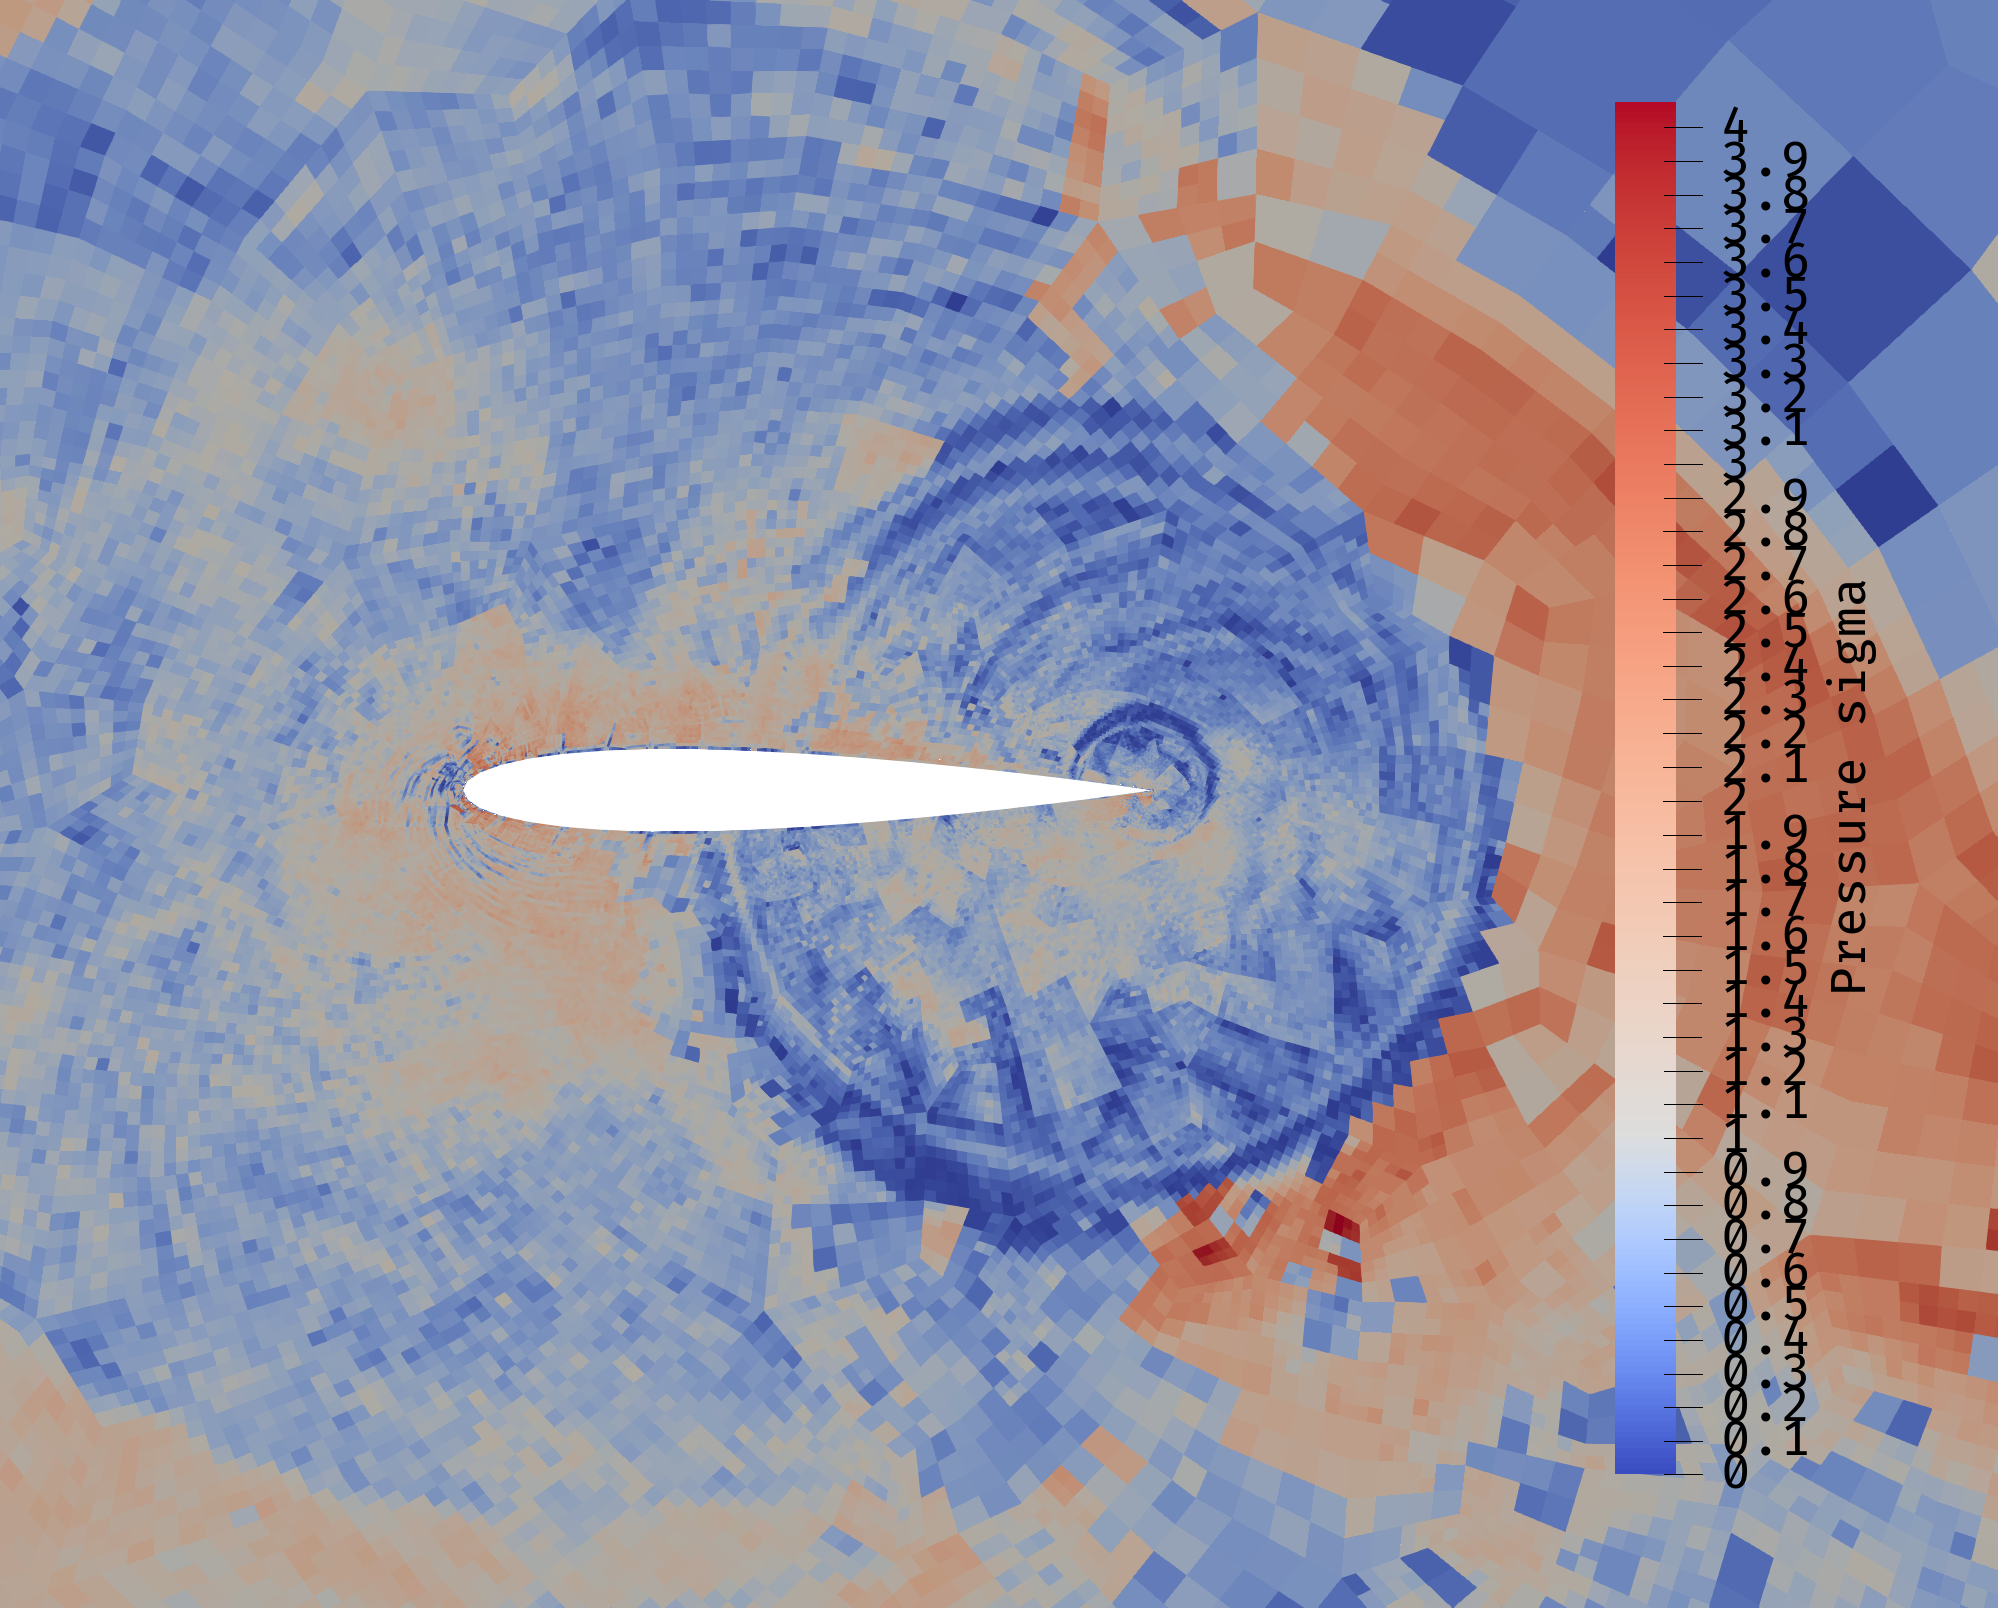
\includegraphics[width=0.48\textwidth]{Chapter_results/media/airfoil_pressure_sigma_near_t1_5}\label{fig:complex_mesh_solution_sigma}}
    
    \smallskip

    \subfloat[Split level]
    {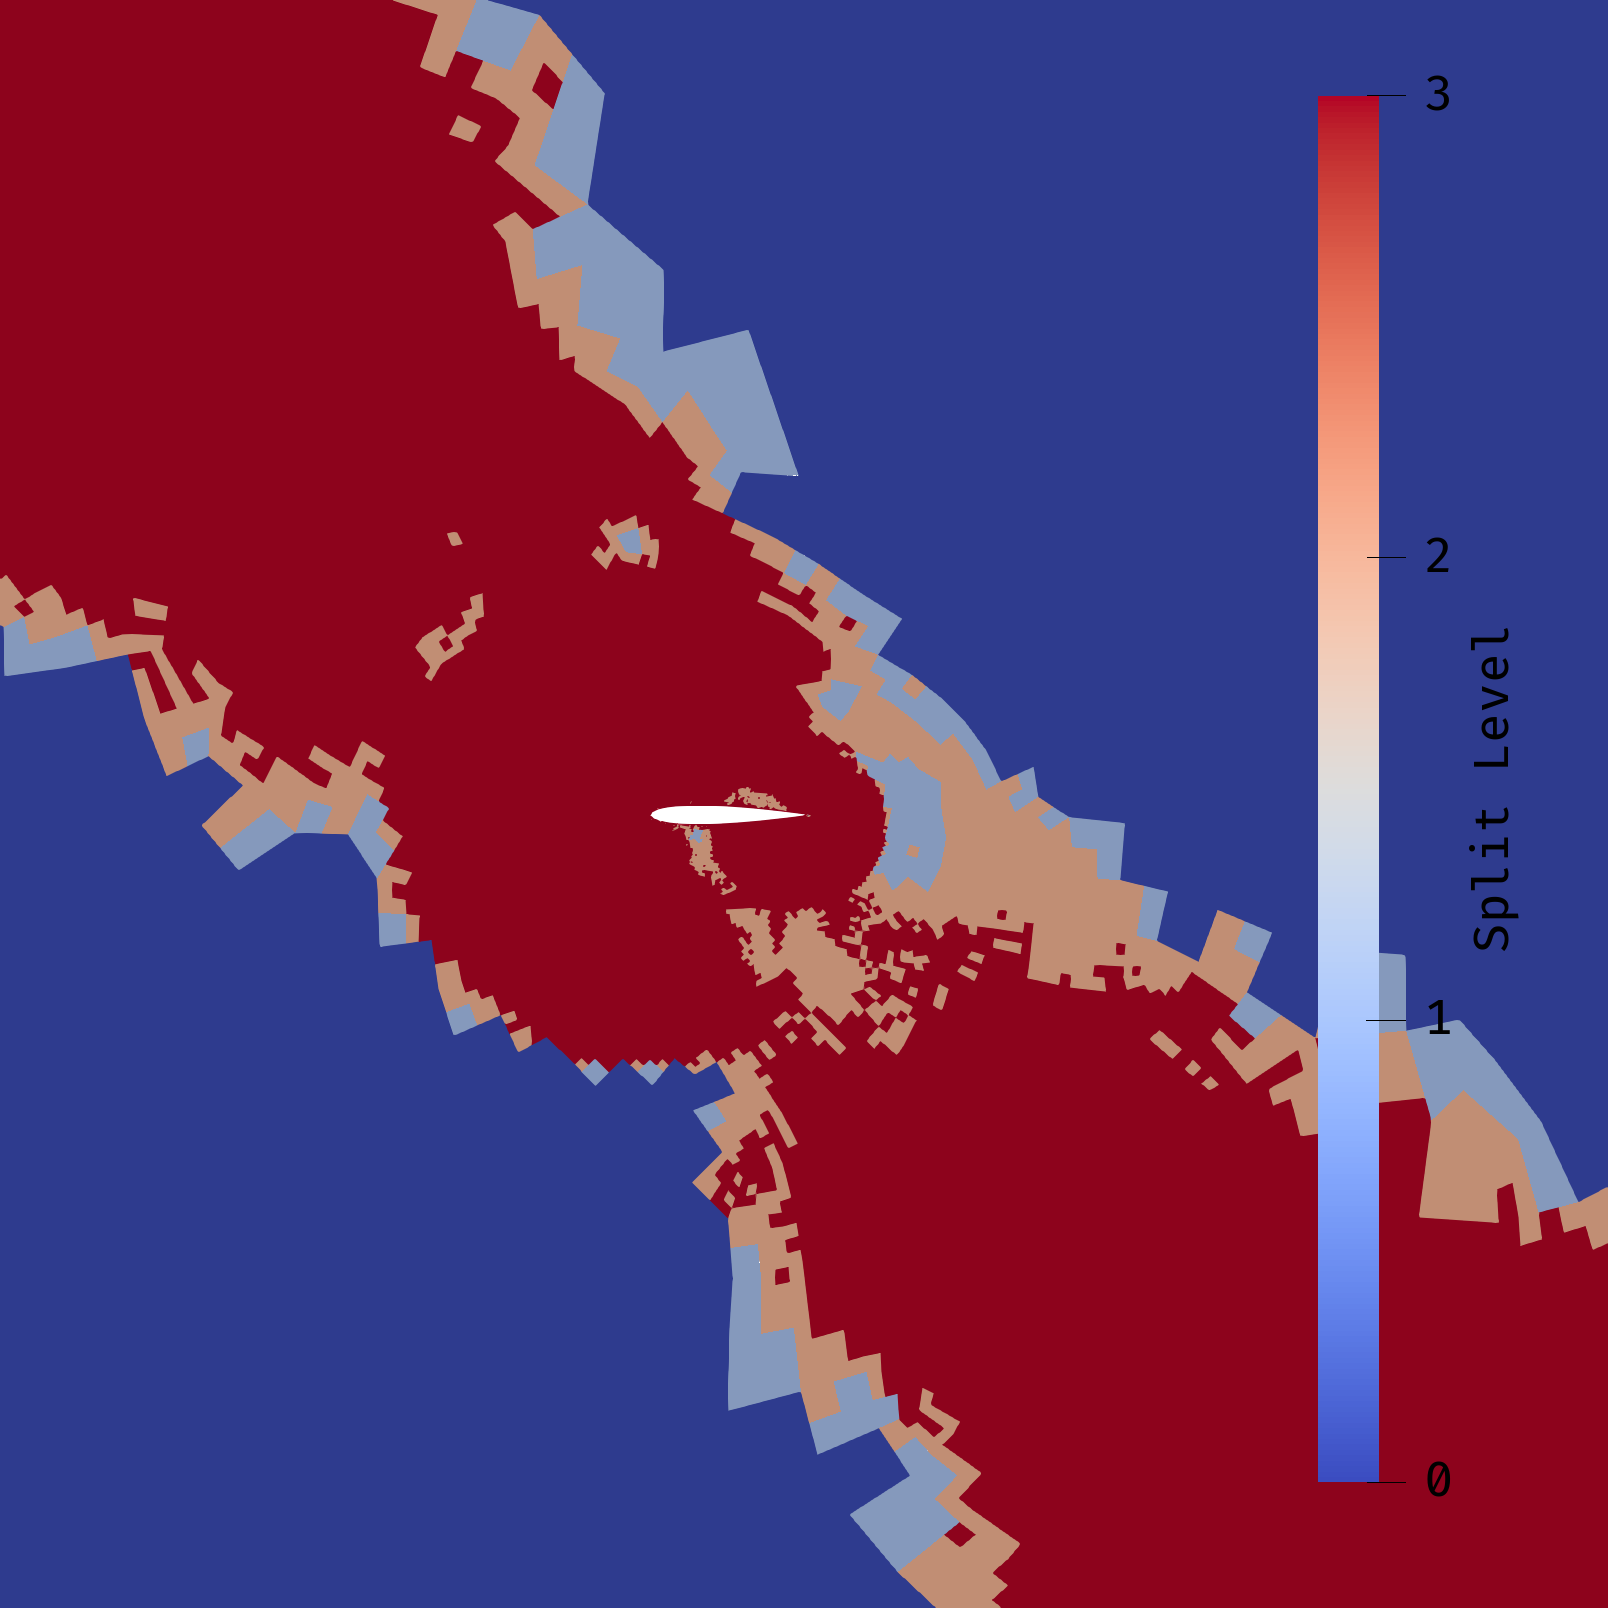
\includegraphics[width=0.48\textwidth]{Chapter_results/media/airfoil_split_level_t1_5}\label{fig:complex_mesh_split_level}}
    \hfill
    \subfloat[N]
    {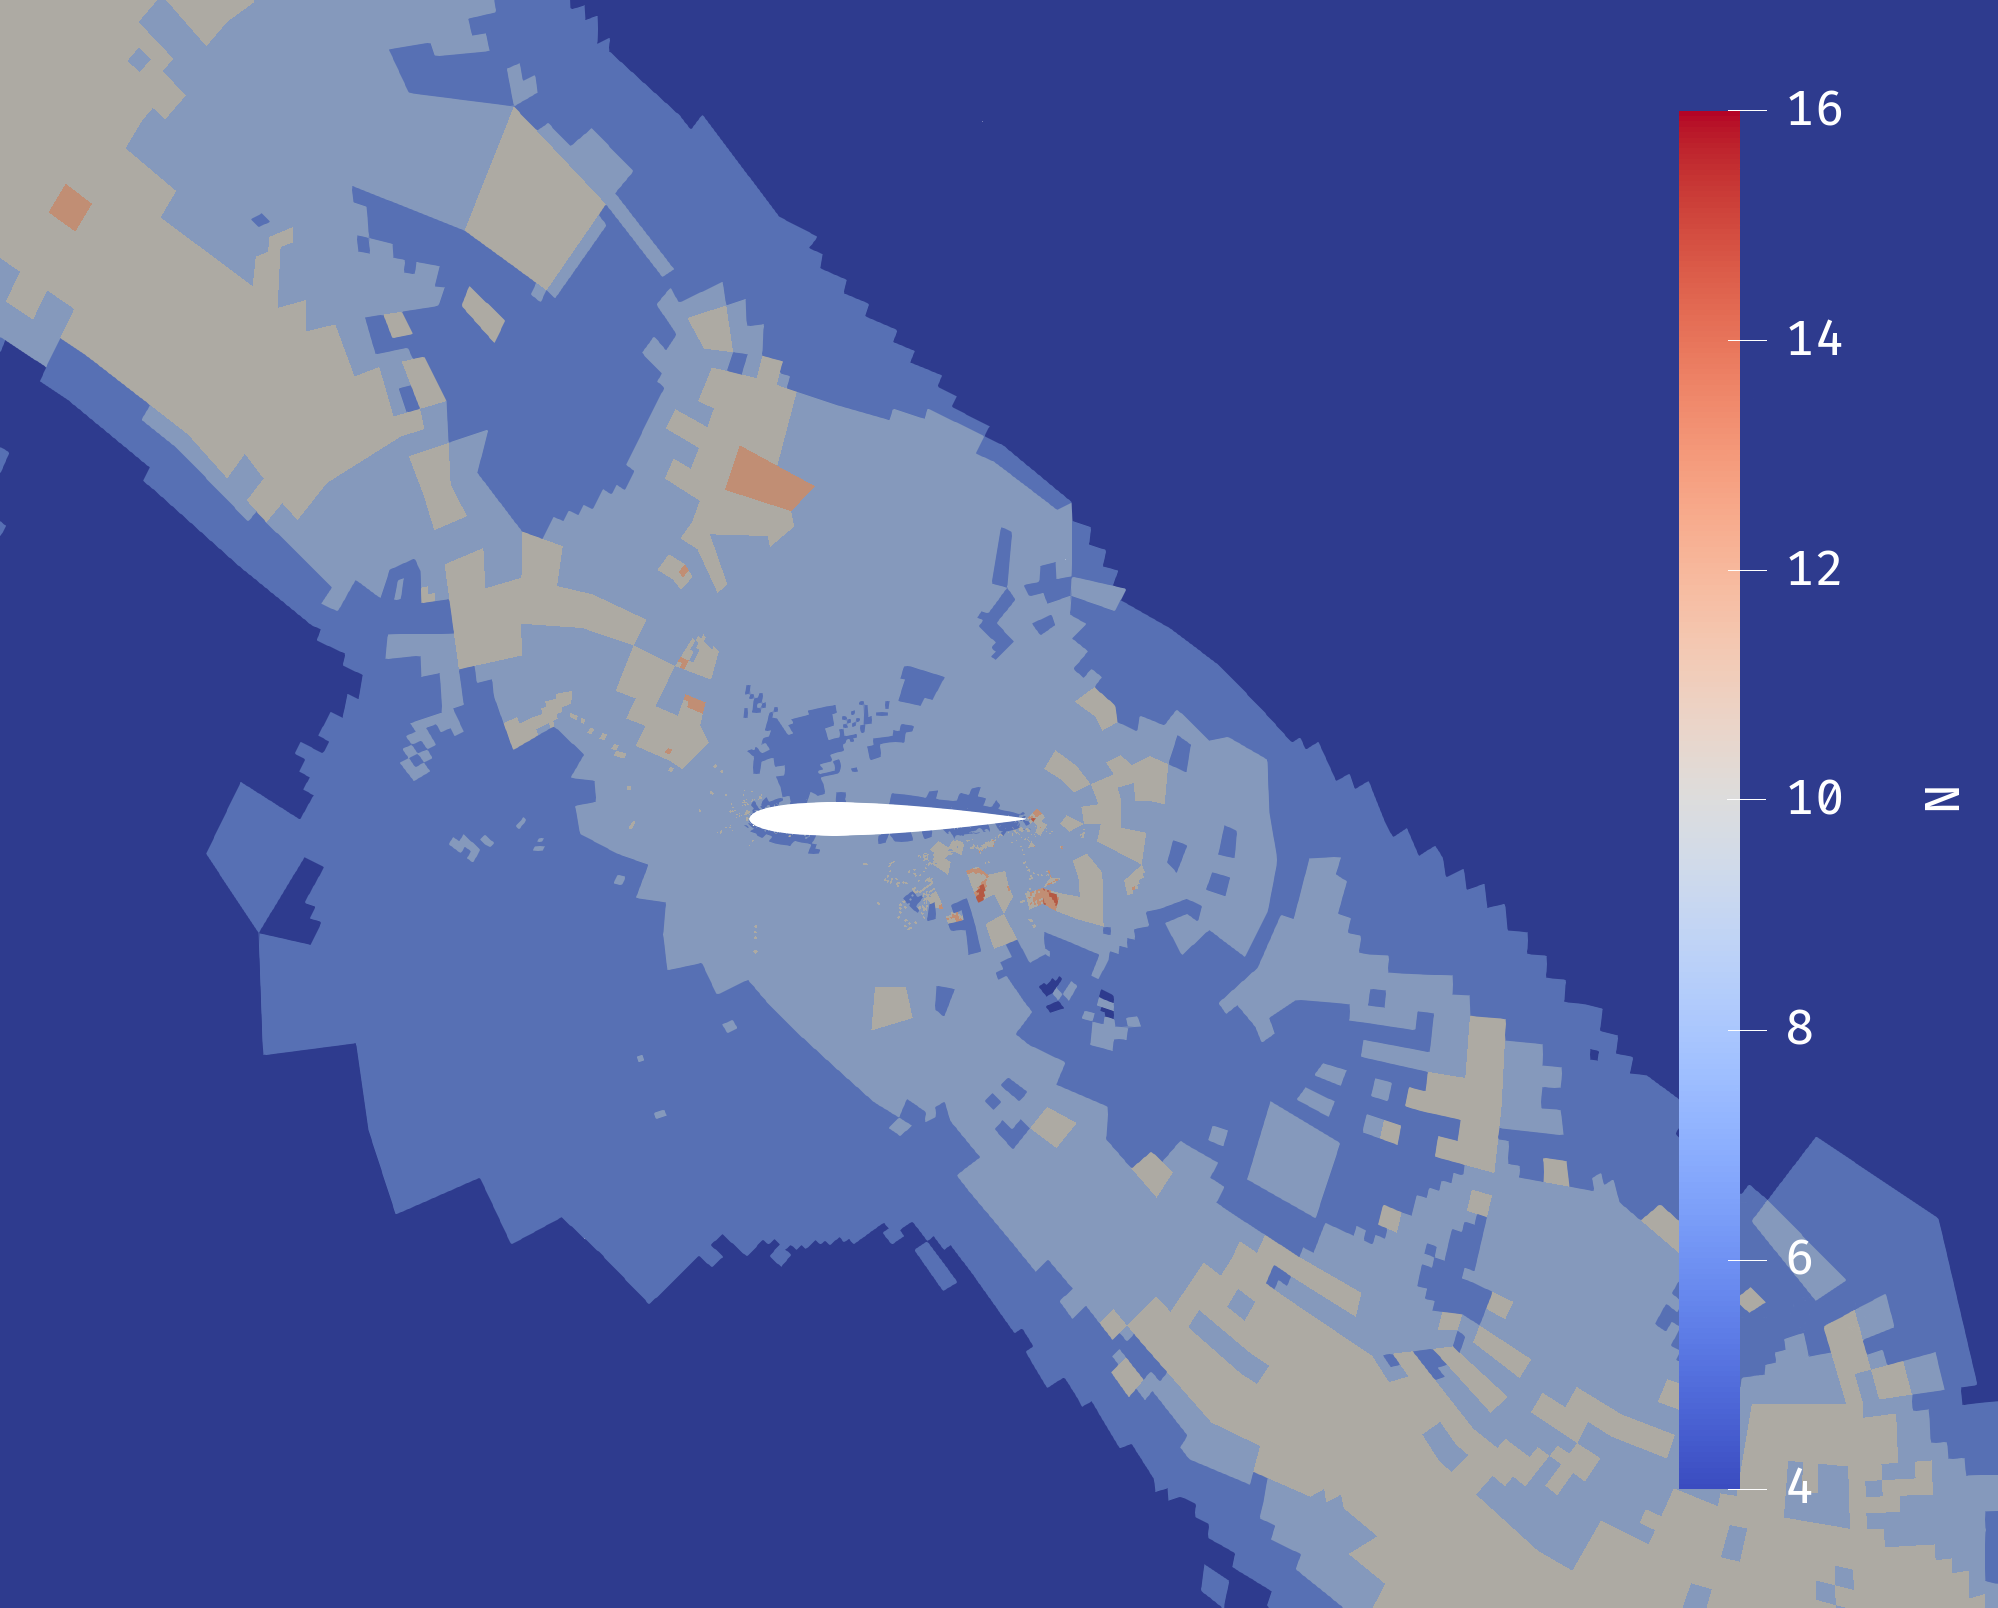
\includegraphics[width=0.48\textwidth]{Chapter_results/media/airfoil_N_t1_5_MOD}\label{fig:complex_mesh_N}}

    \caption{Complex mesh: A wave impinging on an airfoil at \(t = 1.5 s\). \(N_{initial} = 4\), \(K = 55680\), \(S = 3\), \(P = 4\) (a) Pressure (b) Pressure \(\sigma \), prescribing h-refinement or p-refinement (c) h-refinement, the split level denotes how many times elements have split (d) p-refinement, polynomial order \(N\)}\label{fig:complex_mesh_solution}
\end{figure}

Figure~\ref{fig:complex_mesh_solution} shows that the program has refined the mesh in more difficult
areas of the domain, such as along the linear wave, close to the airfoil, and inside the circular
wave. This is consistent with the fact that the interactions between the wave and the airfoil would
create steeper areas in the pressure distribution.

This also shows that the program is able to compute solutions on complex geometries, including
unstructured meshes where elements can be different from axis-aligned squares.

Figure~\ref{fig:complex_mesh_elements} shows how the elements are arranged among the four
\acrshortpl{acr:GPU}. Figure~\ref{fig:complex_mesh_index} shows the indices of the elements, or how
the elements are ordered along the pseudo-Hilbert curve. Figure~\ref{fig:complex_mesh_elements}
shows the elements' rank, or in which \acrshort{acr:GPU} they are stored.

\begin{figure}[H]
    \centering
    \subfloat[Element index]
    {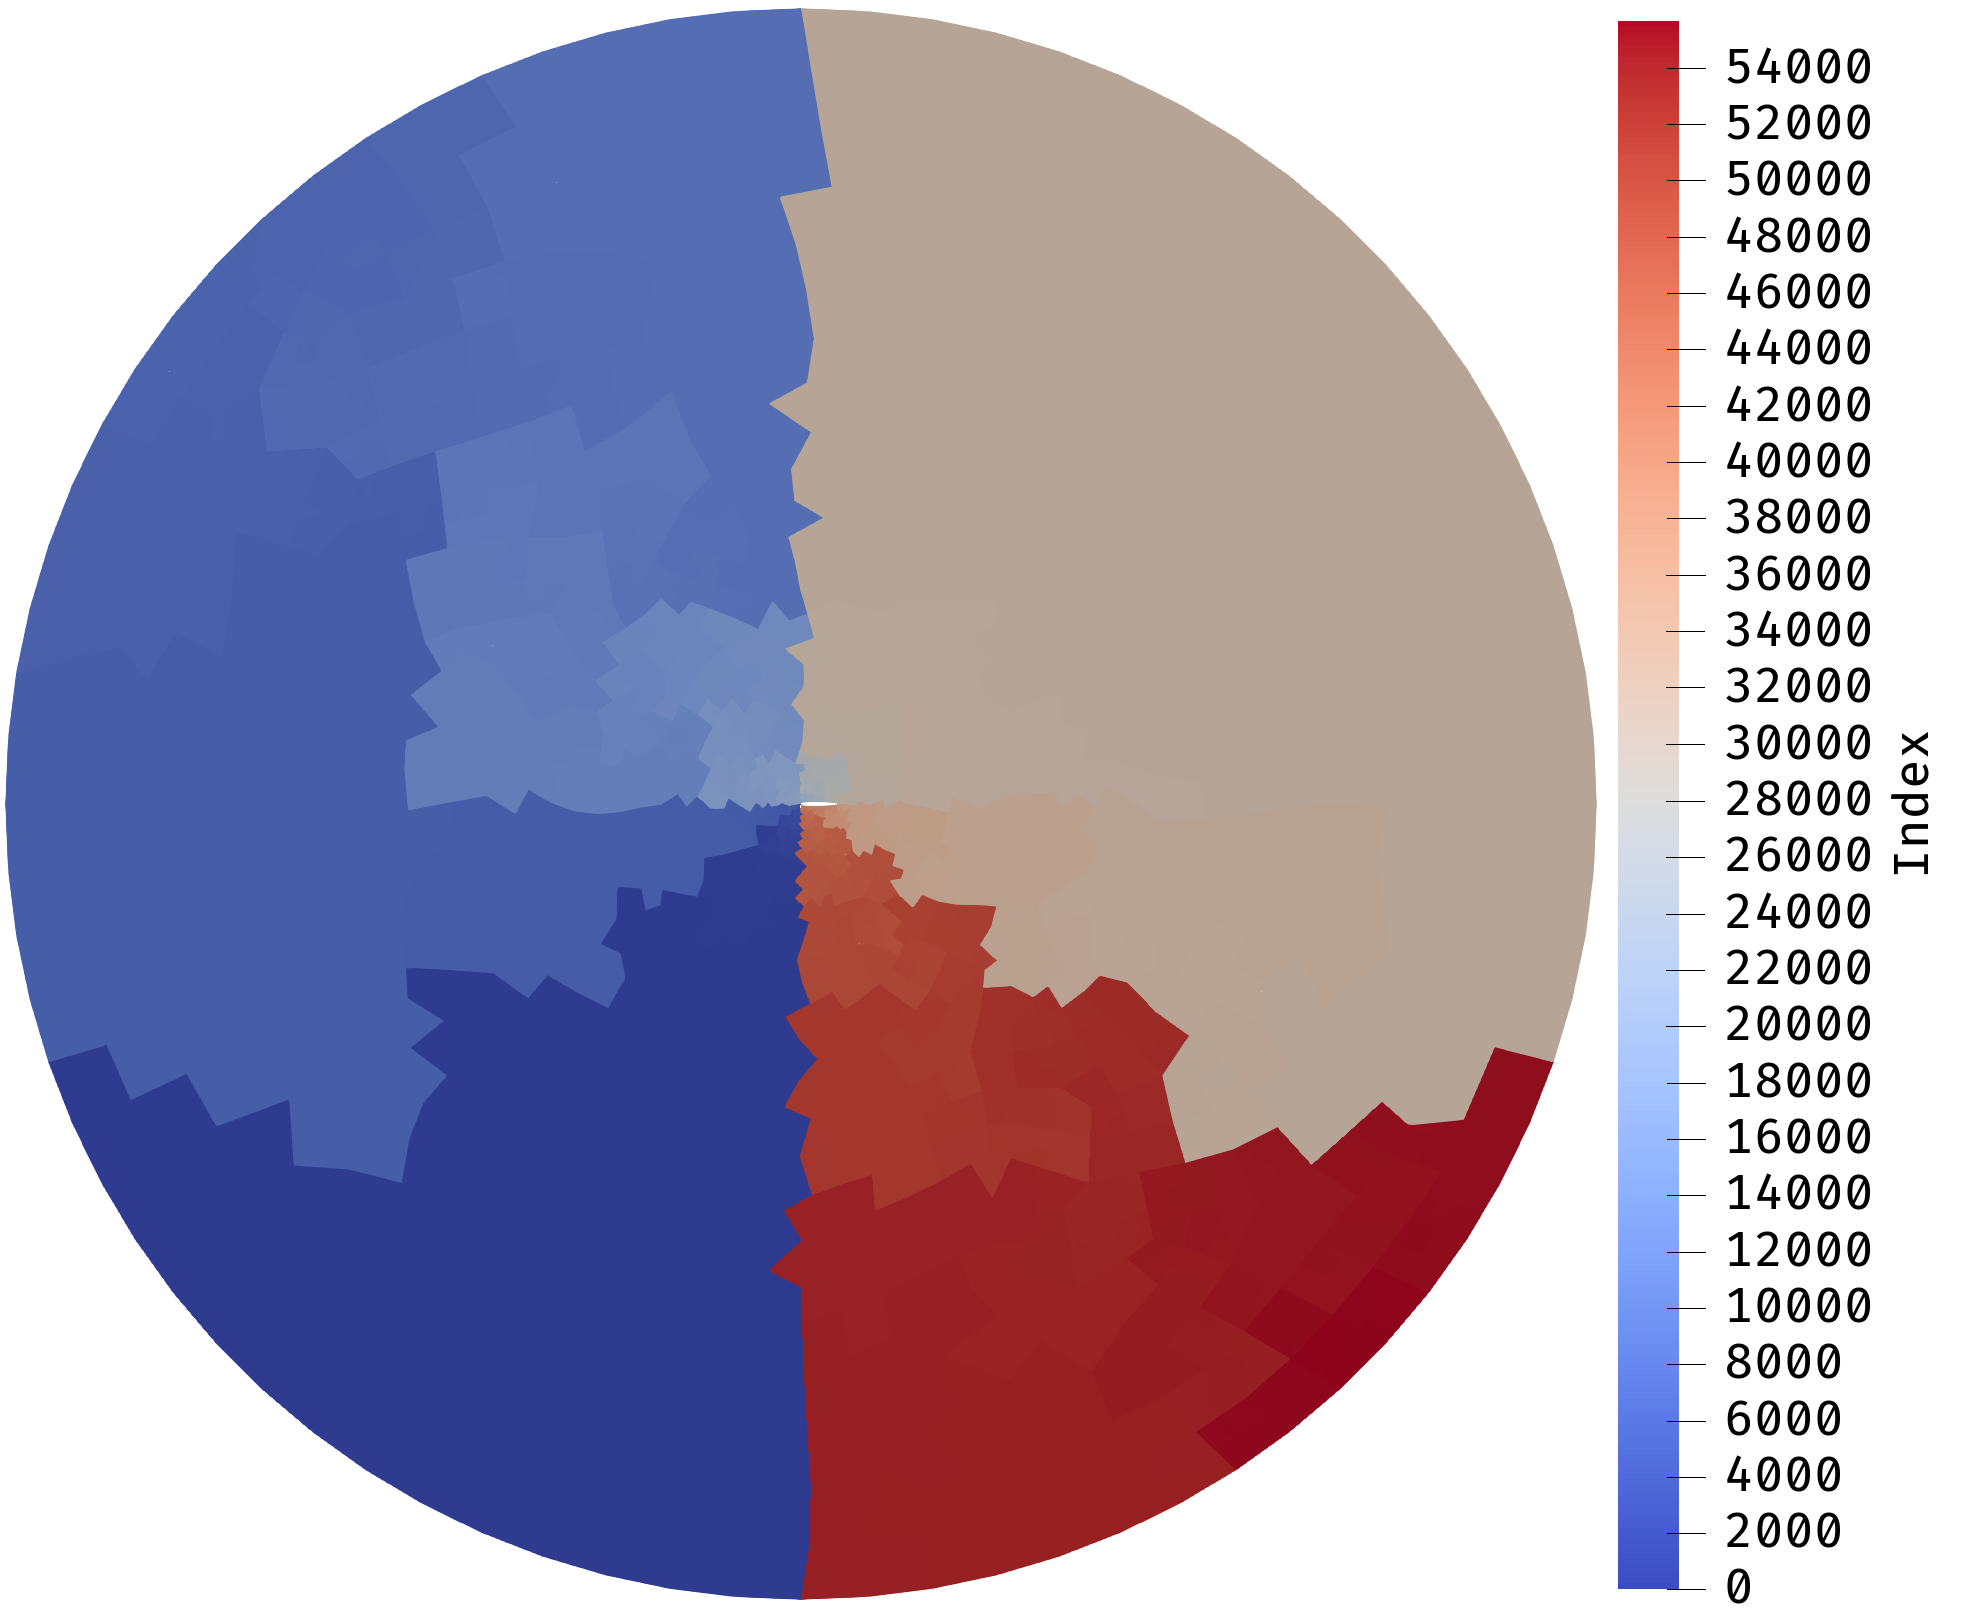
\includegraphics[width=0.48\textwidth]{Chapter_results/media/airfoil_index_t1_5_single}\label{fig:complex_mesh_index}}
    \hfill
    \subfloat[Rank]
    {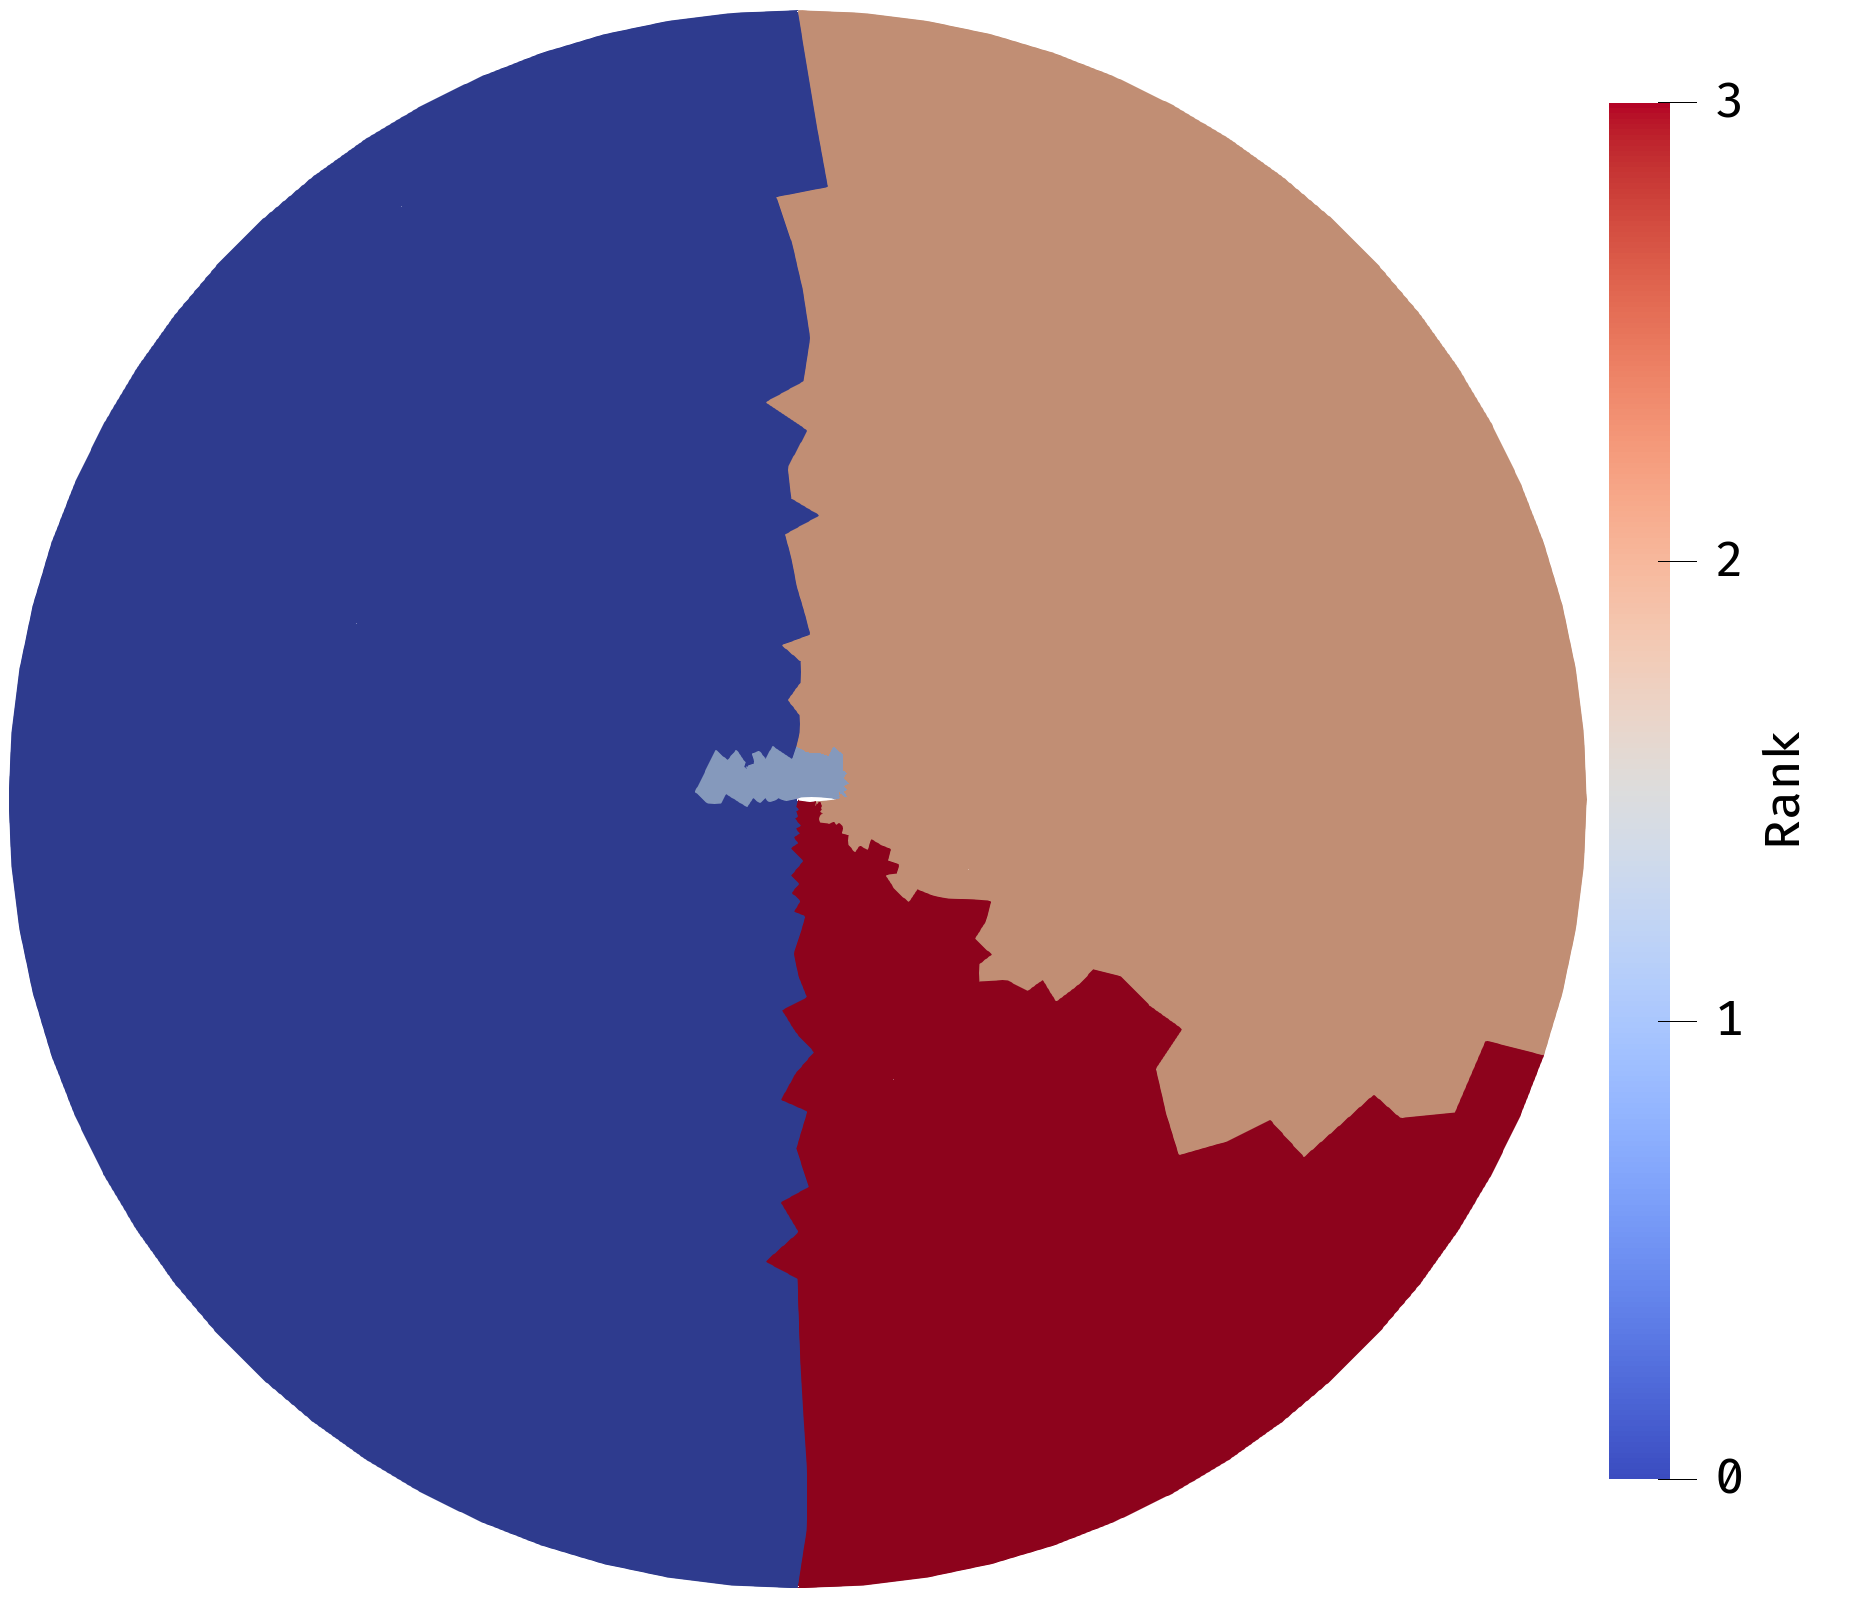
\includegraphics[width=0.48\textwidth]{Chapter_results/media/airfoil_rank_t1_5}\label{fig:complex_mesh_rank}}
    \caption{Element distribution: How elements are distributed between \acrshortpl{acr:GPU}. \(N_{initial} = 4\), \(K = 55680\), \(S = 3\), \(P = 4\) (a) Element indices, showing how they are ordered along the pseudo-Hilbert curve (b) Rank, showing which \acrshort{acr:GPU} contains which elements}\label{fig:complex_mesh_elements}
\end{figure}

On Figure~\ref{fig:complex_mesh_elements}, we can observe that the pseudo-Hilbert curve gives good
locality to the elements, there are few discontinuities between elements, and the surface area
between \acrshortpl{acr:GPU} is small. The elements are well divided between the
\acrshortpl{acr:GPU}, as the \acrshortpl{acr:GPU} in more heavily refined areas have a smaller
footprint in the domain.

\subsection{Profiling}\label{subsection:results:complex_meshes:profiling}

This complex case was also profiled in order to assess which parts of the program were more
computationally intensive. The simulation was run on four \acrshortpl{acr:GPU} up to \(t = 1 s\)
simulation time, refining every \(1000\) time steps and load balancing with a threshold of \(L =
1.1\). Table~\ref{table:profiling} shows the result of this profiling session. This is a report of
\acrshort{acr:GPU} time spent in the different kernels of the program. The report has a resolution
of \(0.1 \% \), therefore most smaller kernels are not shown here. This could artificially reduce
slightly the apparent time spent load balancing the mesh, as the load balancing module is made up of
many smaller kernels, which may not show up in the report. The numbers are the average time spent
between the four \acrshortpl{acr:GPU}. There may also be profiler overhead, especially when memory
is allocated and deallocated. This overhead could artificially inflate the time spent in memory
allocation heavy parts of the program like \acrshort{acr:AMR} and load balancing.

\begin{table}[H]
    \centering
    \begin{tabular}{ c c c c }
        Module & Time proportion (\%) & Algorithm & Time proportion (\%) \\
        \toprule
        \multirow{9}{*}{Solver} & \multirow{9}{*}{\(59.7\)} & compute\_derivative & \(26.68\) \\
                                                          & & project\_to\_elements & \(19.2\) \\
                                                          & & interpolate\_to\_edges & \(7.73\) \\
                                                          & & rk3\_step & \(3.75\) \\
                                                          & & project\_to\_faces & \(1.35\) \\
                                                          & & boundary\_conditions & \(0.37\) \\
                                                          & & compute\_fluxes & \(0.35\) \\
                                                          & & mpi\_interfaces & \(0.2\) \\
                                                          & & reduce\_delta\_t & \(<0.1\) \\
        \midrule
        \multirow{6}{*}{\Acrshort{acr:AMR}} & \multirow{6}{*}{\(38.5\)} & hp\_adapt & \(32.43\) \\
                                                                      & & split\_faces & \(2.63\) \\
                                                                      & & split\_mpi\_interfaces & \(2.55\) \\
                                                                      & & split\_boundaries & \(0.65\) \\
                                                                      & & p\_adapt & \(0.15\) \\
                                                                      & & estimate\_error & \(<0.1\) \\
        \midrule
        \multirow{3}{*}{Load balancing} & \multirow{3}{*}{\(1.4\)} & fill\_received\_elements & \(1.22\) \\
                                                                 & & create\_mpi\_boundaries & \(0.12\) \\
                                                                 & & create\_neighbours & \(<0.1\) \\
        \midrule
        \multirow{1}{*}{Other} & \multirow{1}{*}{\(0.7\)} & empty\_device\_vector & \(0.73\) \\
    \end{tabular}
    \caption{Program profiling: The relative \acrshort{acr:GPU} computation time spent in the three main modules, along with specific kernels and their relative \acrshort{acr:GPU} computation time.}\label{table:profiling}
\end{table}

This case ended up performing \(281078\) time steps, and took 5h04 to complete. The mesh was refined
281 times. These results show that the majority of the time is spent solving the problem and that
the time spent load balancing the mesh is small. This demonstrates very good performance of the
algorithm, with the only concerning result being the proportion of the computation time spent
refining the mesh. The high time spent in the \acrshort{acr:AMR} routine could be reduced by
refining the mesh less often, at the price of using a worse mesh for longer periods.
Section~\ref{section:conclusion:future_work} discusses a different approach to choose when to refine
the mesh which could improve these situations by only refining the mesh when a global target error
threshold is met.
